% arara: pdflatex
% arara: pdflatex
% arara: pdflatex

% options:
% thesis=B bachelor's thesis
% thesis=M master's thesis
% czech thesis in Czech language
% slovak thesis in Slovak language
% english thesis in English language
% hidelinks remove colour boxes around hyperlinks

\documentclass[thesis=B,czech]{FITthesis}[2019/03/21]

\usepackage[utf8]{inputenc} % LaTeX source encoded as UTF-8

% \usepackage{amsmath} %advanced maths
% \usepackage{amssymb} %additional math symbols

\usepackage{dirtree} %directory tree visualisation

% % list of acronyms
% \usepackage[acronym,nonumberlist,toc,numberedsection=autolabel]{glossaries}
% \iflanguage{czech}{\renewcommand*{\acronymname}{Seznam pou{\v z}it{\' y}ch zkratek}}{}
% \makeglossaries

\newcommand{\tg}{\mathop{\mathrm{tg}}} %cesky tangens
\newcommand{\cotg}{\mathop{\mathrm{cotg}}} %cesky cotangens

\usepackage[T1]{fontenc}

\hyphenation{de-ve-lop-ment}
\hyphenation{výs-kyt}
\hyphenation{pří-le-ži-tos-ti}
\hyphenation{pří-le-ži-tost}
\hyphenation{změ-ně}

\usepackage[obeyFinal]{todonotes}
\usepackage[style=iso-numeric]{biblatex}
\addbibresource{mybibliographyfile.bib}
\setcounter{biburllcpenalty}{7000}

% % % % % % % % % % % % % % % % % % % % % % % % % % % % % % 
% ODTUD DAL VSE ZMENTE
% % % % % % % % % % % % % % % % % % % % % % % % % % % % % % 

\department{Katedra aplikované matematiky}
\title{Arbitrážní příležitosti kryptoměn}
\authorGN{Čeněk} %(křestní) jméno (jména) autora
\authorFN{Žid} %příjmení autora
\authorWithDegrees{Čeněk Žid} %jméno autora včetně současných akademických titulů
\author{Čeněk Žid} %jméno autora bez akademických titulů
\supervisor{Mgr. Jan Starý, Ph.D.}
\acknowledgements{Doplňte, máte-li komu a~za co děkovat. V~opačném případě úplně odstraňte tento příkaz.}
\abstractCS{
Tato bakalářská práce se zabývá analýzou arbitrážních příležitostí. Rešeršní část práce se zaměřuje na problematiku bitcoinu, jeho historii, technologie a základní principy. Dále práce popisuje rozdíly mezi několika kryptoměnovými burzami a rozebírá různé druhy arbitrážních příležitostí.

Praktická část práce dále navazuje výběrem nejvhodnější burzy, problematikou dostupností a sběru dat a jejich následným zpracováním.

Analytická část se s pomocí tabulek a grafů, vytvořených z reálných dat, zabývá základními statistikami výskytu a výnosnosti trojúhelníkových arbitrážních příležitostí. Statistiky jsou následně zhodnoceny a jsou vyselektovány nejvýnosnější trojúhelníky. 
}
\abstractEN{
This thesis deals with the analysis of arbitrage opportunities. The theoretical part of the thesis focuses on the bitcoin, its history, technologies and basic principles. The thesis further describes the differences among several cryptocurrency exchanges and narrates about the various types of the arbitrage opportunities. 

The practical part follows up with a selection of the suitable cryptocurrency exchange. In the next part the problematic of data availability and its furhter processing is described. 

The analytic part focuses on the basic statistics of the occurence and profitability of the triangle arbitrage opportunities. These statistics are based on the charts and tables created from the collected data. The statistics are further more evaluated and the most profitable triangles are selected.
}
\placeForDeclarationOfAuthenticity{V~Praze}
\declarationOfAuthenticityOption{4} %volba Prohlášení (číslo 1-6)
\keywordsCS{kryptoměna, analýza dat,  arbitrážní příležitost, kryptoměnová burza, Python, Matplotlib, C++ \newpage}
\keywordsEN{cryptocurrency, data analysis, arbitrage opportunities, cryptocurrency exchange, Python, Matplotlib, C++}
% \website{http://site.example/thesis} %volitelná URL práce, objeví se~v~tiráži - úplně odstraňte, nemáte-li URL práce

\begin{document}


% \newacronym{CVUT}{{\v C}VUT}{{\v C}esk{\' e} vysok{\' e} u{\v c}en{\' i} technick{\' e} v~Praze}
% \newacronym{FIT}{FIT}{Fakulta informa{\v c}n{\' i}ch technologi{\' i}}

\begin{introduction}
% \todo[]{ nezapomeň napsat/smazat poděkování}
% \todo[]{V celé práci je hodně odstavců na 2 řádky. Někdy bych zvážil spojení do většího odstace - vypadá to divně. říká se, že odstavec jsou minimálne 3 řádky}
\todo[]{Citac č. 35 nemá datum citace}
V této práci se zabývám arbitrážními příležitostmi kryptoměn. Jedná se~o téma v~dnešní době velmi aktuální a~moderní. Za~posledních několik let vzniklo velké množství kryptoměn a~žádná z~nich není stabilní. Díky této volatilitě na~burzách s~kryptoměnami vzniká velké množství arbitrážních příležitostí, jejichž analýze se~budu v~této práci věnovat.

Význam této práce spočívá v~analýze jednotlivých burz jako takových. Práce se~také zabývá otázkami, jak často se~reálně objevují arbitrážní \linebreak příležitosti v~rámci jednotlivých burz, jak dlouho trvá, než tyto příležitosti zmizí, a~jestli je možné nacházet arbitrážní příležitosti v rámci vybrané burzy.

Toto téma jsem vybral především, protože mě baví \todo[]{DPR mi vytýkali citově zabarvený slova} analyzovat data a~snažit se~najít výstupy, které je možné z~dat vytěžit. Zároveň z~toho důvodu, že dat týkajících se~kryptoměn je na~internetu k~dispozici velké množství, jsou jednoduše dostupná a~dají se~na~nich zjistit zajímavé výstupy. Výhodou arbitrážních příležitostí je to, že se~jedná o~transakce víceméně bez rizika, na~rozdíl od~klasického obchodování s~kryptoměnami, kde je většinou riziko velké a~o jistotě se~mluvit nedá. Z~toho důvodu mi připadá velice zajímavé tyto arbitráže zkoumat podrobněji. 

V práci se~zabývám dostupností dat v~rámci jednotlivých kryptoměnových burz a~možnostmi ukládání těchto dat. Dále se~v~práci zabývám analýzou dat a analýzou výskytů korelací, které v~rámci burz nastávají.

V první části práce se~věnuji tomu, co to jsou kryptoměny a~co znamenají arbitrážní příležitosti. V~následující části se~věnuji zkoumání dostupnosti dat na~jednotlivých burzách a~možnostem jejich získávání. Na~to navazuji analýzou získaných dat z~pohledu arbitrážních příležitostí. Zabývám se~zde převážně otázkami, jak často arbitrážní příležitosti nastávají a~jestli je reálně možné a~vyplatí se~snažit se~arbitrážní příležitosti vytěžit.

Tato bakalářská práce volně navazuje na~diplomovou práci Adama Pečeva s~tématem Cryptocurrencies Exchange Rates Reporting Tool, ve~které autor vytvořil program, který zobrazuje data jednotlivých kryptoměn na~různých trzích. Já se na rozdíl od~něho více zaměřuji na~analýzu dat.
\end{introduction}

\chapter{Cíl práce}
Hlavním cílem této práce je najít a~analyzovat arbitrážní příležitosti na~historických datech z~kryptoměnových burz a~spočítat statistiky výskytu, obchodovatelnosti a~výnosnosti. 

V teoretické části se~zaměřím na~to, kde je možné historická data týkající se~kryptoměn najít a~získat. Popíšu zde, co jsou to kryptoměny a~arbitrážní příležitosti. Dále se~budu zabývat tím, jakými matematickými a~informatickými metodami je možné tato data analyzovat a~vyberu ty metody, které se~budou na~moji problematiku hodit nejvíce.

V praktické části naimplementuji sběr dat na~úrovni order book jednotlivých měnových párů. Dále na~těchto datech provedu analýzu, kde využiji metody, popsané v~teoretické části. Zhodnotím jaké metody byly účinnější a~vhodnější pro analýzu dat z~kryptoměnových burz a~jaké výsledky jsem vypozoroval.

V závěru praktické části zhodnotím výsledky z~analýzy dat, a~z~vyhodnocených výsledků spočítám základní statistiky výskytu, obchodovatelnosti a~výnosnosti arbitrážních příležitostí. 

\chapter{Současný stav řešení problému}
V této kapitole se~zabývám teorií týkající se~kryptoměn, popisuji základní funkcionalitu transakcí a~technologie blockchainu. Zaměřuji se~na~zmapování jednotlivých kryptoměnových burz. Zaměřuji se~zde také arbitráže, o~co se \linebreak jedná, jaké jsou její druhy a~jak se~projevují na~poli kryptoměnových burz.

\section{Kryptoměny}
V této podkapitole se~obecně zabývám kryptoměnami. Zaměřuji se~na~jejich historii, která je spjatá převážně s~první a~nejhodnotnější kryptoměnou, kterou je bitcoin. Zabývám se~zde také alternativními kryptoměnami. Dalším tématem je krátký úvod do~technologií, na~kterých jsou kryptoměny založeny. \cite{BudoucnostFinTrhu}

\subsection{Bitcoin - BTC}
Bitcoin je první kryptoměna, která byla zavedena v~roce 2009 anonymní skupinou lidí pod pseudonymem Satoshi Nakamoto. Hlavní myšlenkou bitcoinu je snaha o~odstranění všech regulatorních vlastností měn a~snaha o~zvýšení transparentnosti a~bezpečnosti plateb a~transakcí v~rámci bitcoinové sítě. \cite{Finex}

Hlavní charakteristikou bitcoinu je to, že nemá žádnou centrální autoritu (například pro českou korunu je centrální autoritou Česká národná banka), z~čehož plyne, že s~ním nikdo nemůže manipulovat tak, jako s~běžnými měnami.

Jednou z~předních výhod je to, že transakce trvají řádově desítky minut, což v~porovnání s~bankami je v~průměru rychlejší. Bitcoin také není možné zfalšovat, neboť je vše naprosto transparentně uloženo v~blockchainu.

Na druhou stranu má bitcoin i~řadu nevýhod oproti běžným měnám, které také vyplývají z~toho, že nemá žádnou centrální autoritu. Jednou z~hlavních nevýhod je to, že je velice nestabilní oproti běžným měnám a~v~žádnou chvíli nelze s~velkou pravděpodobností předpovídat, jak se~bude jeho hodnota vyvíjet. \cite{Finex}

\subsubsection{Blockchain}
Bitcoin je založen na~technologii blockchainu. Blockchain je možné si představit jako veřejně sdílenou účetní knihu, ve~které jsou zachyceny veškeré transakce, které kdy proběhly. Konkrétně se~jedná o~distribuovanou decentralizovanou databázi, která uchovává chronologický řetězec záznamů. Principem je, že tyto data jsou v~blockchainu uchovány napořád a~jsou veřejně dostupná pro všechny, tudíž je není možné nijakým způsobem změnit nebo zfalšovat. \cite{Bitcoin_how_it_works}

Základní myšlenkou blochchainu je to, že je připraven o~jakoukoli centrální autoritu (například banku). Z~toho důvodu není možné s~ním nijak centrálně manipulovat ani jakkoliv ovlivňovat jeho historii.
\hyphenation{Tran-sak-ce}
Blockchain se~skládá ze~dvou druhů záznamů, z~transakcí a~z~bloků. Transakce jsou tvořeny uživateli, kteří chtějí například převádět kryptoměnu. Bloky tyto transakce potvrzují \linebreak a~shromažďují a~řadí do~chronologické posloupnosti. \cite{Finex_blockchain}

\subsubsection{Těžení}
Těžení je velmi důležitým procesem v~rámci blockchainu. Nové bloky jsou přidávány periodicky (většinou každých několik minut). Těžaři v~rámci těžení přidávají jednotlivé transakce do~následujícího bloku. Veškeré transakce, které jsou do~bloku přidány jsou tímto procesem potvrzeny. 

Těžení je jakási soutěž mezi všemi těžaři, ve~které se~každý snaží uspět za~cílem získání odměny za~vytěžení daného bloku včetně s~poplatky za~přidaní jednotlivých transakcí do~blockchainu.

Těžení zajišťuje také bezpečnost blockchainu, neboť těžení je matematicky velmi náročný proces a~jakýkoliv pokus o~zfalšování původních dat se~stává s~každým blokem o~poznání náročnější. \cite{mastering_bitcoin}

\subsubsection{Transakce}
Transakce je převod peněz z jedné adresy na jinou. Tyto transakce jsou volně předávány od~uzlu k~uzlu. Těžaři se~mezitím snaží vytvořit blok, který se~zajistí o~to, aby byly transakce potvrzeny a~považovány za~validní.

Adresa je unikátní řetězec znaků jednostranně odvozen z veřejného klíče konkrétního uživatele, není tedy možné zjistit, jaká adresa odpovídá, kterému uživateli. Adresa je poté využita v~rámci transakcí v~roli odesilatele nebo příjemce. \cite{mastering_bitcoin}

Za validní transakci je považována taková transakce, která splňuje \linebreak následující podmínky: je v~ní obsažen správný elektronický podpis uživatele, uběhla adekvátně dlouhá doba od~poslední transakce s~tímto kusem měny. \cite{Finex_blockchain}

Dalším téměř nutným požadavkem je zahrnutí nějakého poplatku pro těžaře za~to, aby transakci zahrnul do~dalšího bloku. Těžař si ponechává poplatky všech transakcí, které do~vytěženého bloku zahrnul, a~proto nemá motivaci zahrnovat transakci bez poplatku. \cite{Finex_blockchain}

\subsection{Altcoiny}
Pojmem altcoin se~označují všechny ostatní kryptoměny podobné bitcoinu. Název je odvozen z~anglického pojmu alternative to bitcoin. Některé altcoiny jsou svojí techonologií a~principem hodně podobné bitcoinu, jsou ale i~takové, které se~poměrně výrazně liší. \cite{pecev}

V následujících podkapitolách se~zaměřím na~nejvýznamnější zástupce altcoinů a~vypíši zde všechny altcoiny, kterým se~ve své praktické části této práce věnuji.

\subsubsection{Litecoin - LTC}
Litecoin je jedním z~nejstarších altcoinů. Tato open source měna vznikla v~roce 2011 a~je svou charakteristikou velmi podobná svému předchůdci. \cite{litecoin} Dokonce i~celý kód je pouze úpravou bitcoinu. \cite{alza_monero}

Hlavní rozdíl mezi litecoinem a~bitcoinem je ten, že litecoin byl od~počátku navržen tak, aby lépe zvládal větší počty transakcí a~aby transakce probíhaly ještě rychleji. Díky této vlastnosti se~stal výhodnější pro menší transakce. Všechny tyto charakteristiky jsou založeny na~tom, že jsou bloky přidávány čtyřikrát rychleji, než je tomu u~bitcoinu. \cite{litecoin} Cena za~jeden litecoin dosahuje hodnoty \$~40,63 (údaj ze~4.4. 2020 na~burze Binance). \cite{binance_markets}

\subsubsection{Ethereum - ETH}
Ethereum je stejně jako litecoin open source kryptoměna založená na~technologii blockchainu. Vznik etherea se~datuje k~30. 7. 2015. 

Hlavním rozdílem oproti bitcoinu je to, že se~nejedná o~měnu, ale o~platformu se~svou vlastní měnou Ethereum. Platforma Ethereum tvoří alternativu ke~všem klasickým smlouvám a~dohodám a~snaží se~o zdokonalení chytrých kontraktů. \cite{btc_vs_eth}

Chytrý kontrakt je zjednodušeně program, který se~stará o~provedení smlouvy. Tento program tak nahrazuje třetí stranu (například právníky, či notáře) a~zajišťuje transparentní převedení peněz, majetku nebo čehokoli \linebreak jiného. \cite{ethereum}

Na platformě Ethereum je možné vytvářet tyto vlastní programy. \cite{ethereum} Rozdíl Etherea oproti bitcoinu je ten, že nikdy nedojde k~vytěžení všech mincí, nýbrž budou mince stále emitovány. \cite{alza_monero} Cena za~jedno Ethereum dosahuje hodnoty  \$~142,82 (údaj ze~4.4. 2020 na~burze Binance). \cite{binance_markets}

\subsubsection{Monero - XMR}
Monero po~vzoru svého nejstaršího předchůdce vzniklo jako open source projekt. Samotný kód není vůbec založen na~bitcoinu (na rozdíl od~litecoinu). 

Monero se~pyšní tím, že zaručuje naprostou anonymitu. Historii a~stav konta v~případě Monera si může prohlížet pouze majitel účtu. V~případě bitcoinu všichni vidí, jaké transakce proběhly a~pokud se~tedy podaří identifikovat vlastníka nějaké adresy, je jednoduché dohledat si veškerou historii transakcí, které z~dané adresy byly provedeny .

Stejně jako ostatní kryptoměny, má Monero také dvojici privátního \linebreak a~veřejného klíče, má však ještě druhou dvojici privátního a~veřejného klíče a~to takzvaného klíče k~prohížení (view key). View key je možné poskytnout třetí osobě, aby se~přes něj byla schopna dozvědět veškerou historii transakcí, které na~adrese proběhly, tudíž je možné udělat i~transparentní účet.

Poslední důležitý rozdíl oproti bitcoinu je to, že celkový počet Monera není . Emitování mincí stále nepoběží stejnou rychlostí, ale postupně se~bude snižovat, dokud nedosáhne spodní nenulové hranice. \cite{alza_monero} Cena za~jednu minci Monera dosahuje hodnoty  \$~54,59 (údaj ze~4.4. 2020 na~burze Binance). \cite{binance_markets}

\subsubsection{Ripple - XRP}
Ripple není pouze označení pro kryptoměnu, ale také pro celosvětovou platební síť. Síť Ripple vznikla s~předním účelem osvobození internetových plateb od~poplatků za~směnu, zpracování transakcí a~časových prodlev. Ripple nebere rozdíly mezi tradičními měnami a~kryptoměnami a~tím zlevňuje veškeré výměny mezi nimi.

Ripple je stejně jako výše zmiňované kryptoměny založen na~principu blockchainu. Výrazně se~oproti ostatním liší tím, že všechny jeho mince byly emitovány při vzniku sítě, tedy se~jejich počet nezvyšuje procesem těžení, jako tomu je u~ostatních.

Kvůli tomu, že byly všechny mince emitovány při vzniku, vlastní zakládající společnost Ripple Labs více než polovinu veškerých tokenů. Z~toho důvodu také velmi odporuje úplně původní myšlence bitcoinu a~tedy zásahu jakékoliv třetí strany. \cite{alza_ripple}

Transakce se na rozdíl od ostatních kryptoměn uzavírají na základě konsensu. Síť Ripple však není kontrolována Ripple Labs, ale jedná se o peer-to-peer systém, ve kterém se uživatelé, jakožto uzly, připojují do sítě. Když probíhá transakce mezi některými uzly, ostatní uzly fungují jako validátoři provádějící proces konsesnsu. Validátoři se pomocí RPCA (Ripple Protocol Consensus Algorithm) algoritmu domluví na aktuálním stavu účetní knihy a přidají validní transakce do sady kandidátů. Následně se o~těchto kandidátech hlasuje a ti kandidáti, kteří překročí minimální 80\% hranici, jsou přidáni do účetní knihy. \cite{RPCA}

Díky tomu, že se~transakce uzavírají na~základě konsensu a~také díky tomu, probíhají transakce řádově rychleji, v~řádech několika vteřin. Poplatky jsou taktéž minimální, většinou méně než 0.001~USD. \cite{bitinfocharts} \cite{coincodex_ripple}

\subsubsection{Ostatní zpracovávané altcoiny}
V předchozí části jsem zmínil nějaké dle mého názoru významné a~zajímavé altcoiny. Ve~své práci však potřebuji více kryptoměn, nad kterými budu pracovat. Proto jsem vybral ještě následující kryptoměny.

\textbf{Bitcoin Cash (BCH)} je kryptoměna, která vznikla odvětvením od~bitcoinu, z~důvodu obav přehlcení sítě. Je tedy se~svým předchůdcem téměř totožná, co se~týče základních vlastností. \cite{kurzy_bch}

\textbf{EOS (EOS) je kryptoměna,} která se~podobně jako Ethereum zaměřuje na~využití chytrých kontraktů, kde každý uživatel držící EOS token může využívat \linebreak příslušnou část výpočetní síly a~uložiště. \cite{finex_eos}

\textbf{Binance Coin (BNB)} je interní kryptoměna platformy a~burzy Binance, která vychází ze~standardu platformy Etherea. Binance Coin je dostupný téměř výhradně na~své domovské platformě, kde však má svůj účel. \cite{martin_sistek_bnb}

\textbf{TRON (TRX)} je kryptoměna vytvořena za~účelem decentralizace sdílení informací na~internetu převážně multimediálního obsahu (jako jsou například videa, hudba, hry). TRON je schopný zpracovat až 2000 transakcí za~sekundu a~tím je až osmdesátkrát rychlejší než jeho konkurent Ethereum. \cite{finex_trx}

\textbf{USD Tether (USDT)} je zástupce stable coinu (stabilní měny), jeho cena je vázaná na~běžnou měnu, v~tomto případě na~americký dolar. USD Tether je nejznámějším zástupcem stabilní měny, který je využíván velkým množstvím burz (například Binance, Huobi, Okex) a~jeho celková kapitalizace je více než 2 miliardy amerických dolarů. \cite{mlady_investor_stable_coin} 

\section{Kryptoměnové burzy}
\label{cryptocurrency_exchanges}
V této podkapitole se~zaměřuji na~několik kryptoměnových burz. Poukazuji na~jejich klady a~zápory a~věnuji se~výběru těch nejlepších mezi nimi.

\subsection{Coinmate}
Coinmate je kryptoměnová burza sídlící ve~Velké Británii, která vznikla \linebreak na~základě technologií české společnosti Profinit v~roce 2014. Burza se~zaměřuje na~tyto tři základní aspekty: rychlost, spolehlivost a~bezpečnost. Coinmate se~řadí mezi menší burzy, podle ohlašovaného obchodovaného objemu za~posledních 30~dní ve~velikosti (21~658~191 amerických dolarů \cite{coin360}) se~burza neřadí ani mezi 100 největších. \cite{coinmarketcap} Burza ani nenabízí velké množství obchodovatelných párů, pouze 20. Dříve do 25.3. 2020 bylo možné na Coinmate obchodovat s~Korunou českou a Eurem. Obchodování s Eurem by mělo být možné nejspíš někdy ke konci května nebo v červnu. Coinmate se opět snaží nastavit podmínky tak, aby bylo možné i obchodování s Korunou českou. \cite{coinmate_blog}  

Coinmate se~dále pyšní tím, že má poměrně nízké poplatky. Pro uživatele v~roli "maker", ti kteří aktivně vytvářejí nabídku a~poptávku, činí poplatek 0,12~\% až 0~\% (viz obrázky \ref{coinmate_standard} a~\ref{coinmate_promotional}). Pro uživatele v~roli "taker", ti kteří nevytvářejí nové nabídky a~poptávky, pouze obchodují na~aktuálních, se~poplatek pohybuje v~rozmezí 0,25~\% až 0.05~\% (viz obrázky \ref{coinmate_standard} a~\ref{coinmate_promotional}. Tímto systémem poplatků, kdy má nižší poplatky pro tvůrce trhu (makers), se~snaží burza podpořit likviditu na~trhu. \cite{cryptowisser_coinmate} \cite{coinmate_fees}

Z obrázků \ref{coinmate_standard} a~\ref{coinmate_promotional} je také možné vidět, že poplatky jsou sníženy pro obchodníky, kteří obchodují na~burze s~vyššími objemy, u~maker tak může dojít ke~snížení až na~hranici nulových poplatků. \cite{coinmate_fees}

\begin{figure}\centering
	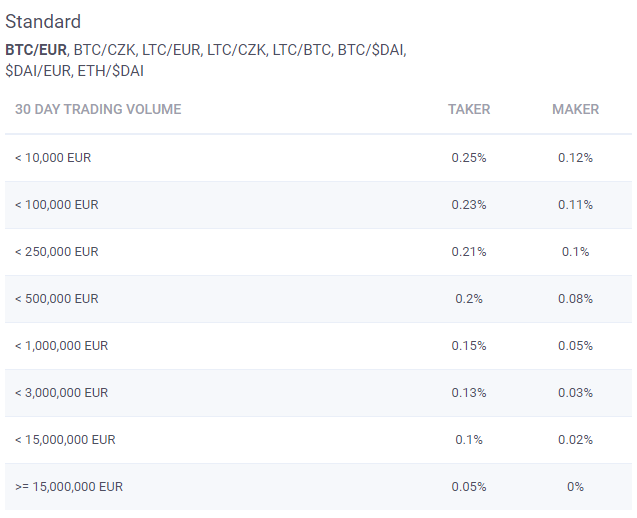
\includegraphics[width=1\textwidth]{images/coinmate_standard.PNG}
	\caption{Poplatky na~burze Coinmate pro maker i~taker) \cite{coinmate_fees}}\label{coinmate_standard}
\end{figure}
\begin{figure}\centering
	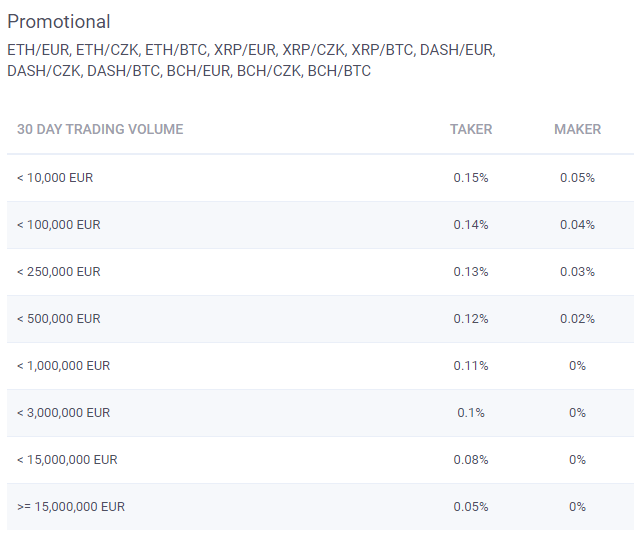
\includegraphics[width=1\textwidth]{images/coinmate_promotional.PNG}
	\caption{Poplatky na~burze Coinmate pro maker i~taker) \cite{coinmate_fees}}\label{coinmate_promotional}
\end{figure}

\todo[]{U tabulek a obrázků můžeš nastavovat plavoucí prostředí. Richtr mi říkal, že se to případně dává tak, aby když tabulka nemůže být na svém přesném místě tak bude dole na stránce (má popisek nahoře) a obrázek nahoře n stránce (má popisek dole). Většinou ty pozice  vychází celkem dobře}

\subsection{Binance}
Burza Binance byla založena v~Číně v~roce 2017, avšak později své sídlo přesunula na~Maltu. Binance je podle dat z~CoinMarketCap největší burzou, co se~týče zobchodovaného objemu za~posledních 30 dní (158~302~486~366 amerických dolarů). \cite{coinmarketcap} Burza podporuje obchodováním s~1320~odlišnými měnami.

Binance je také specifická tím, že všechny obchodovatelné dvojice se  \linebreak sestávají pouze z~kryptoměn a~ne z~běžných měn. Například americké dolary jsou nahrazeny stable coiny, jako je například USDT nebo TUSD. 

Burza Binance si v~průměru účtuje 0.1~\% za~provedené obchody s~měnami. Tento poplatek je stejný jak pro maker tak pro taker. Pokud se~uživatel rozhodne zaplatit tyto poplatky domovskou měnou binance coin (BNB), pak jsou tyto poplatky redukovány o~polovinu. Z~toho plyne, že poplatky na~burze Binance patří k~jedněm z~nejnižších.

Vkladové poplatky jsou nulové pro veškeré měny. Na~druhou stranu \linebreak výběrové poplatky se~liší pro každou měnu (viz obrázek \ref{binance_fees}). \cite{blockonomi_binance}

\begin{table}\centering
    \caption{Výběrové poplatky na~burze Binance \cite{binance_fees}}
    \label{binance_fees}
     \begin{tabular}{||c | c | c | c||} 
     \hline
     Měna/token & Název & Minimální výběr & Výběrový poplatek \\ [0.5ex] 
     \hline\hline
     BTC & Bitcoin & 0,001 & 0,0004 \\ 
     \hline
     LTC & Litecoin & 0,002 & 0,001 \\
     \hline
     ETH & Ethereum & 0,02 & 0,003 \\
     \hline
     XMR & Monero & 0,0002 & 0,0001 \\
     \hline
     XRP & Ripple & 0,5 & 0,25 \\
     \hline
     BCH & Bitcoin Cash & 0,002 & 0,001 \\
     \hline
     EOS & EOS & 0,2 & 0,1 \\
     \hline
     BNB & BNB & 0,12 & 0 \\
     \hline
     TRX & TRON & 2,16 & 1,08 \\
     \hline
     USDT & TetherUS & 1,44 & 0,72 \\
     \hline
    \end{tabular}
\end{table}
\subsection{MXC}
Burza MXC je jednou z~novějších burz. Vznikla v~dubnu roku 2018 a~je registrována v~Singapuru. Podle statistik serveru CoinMarketCap je druhou největší z~pohledu obchodovaného objemu za~posledních 30 dní s~objemem 101~249~688~459 amerických dolarů. \cite{coinmarketcap} MXC podobně jako burza Binance podporuje velké množství altcoinů, celkově je zde možné obchodovat s~264 měnami. \cite{mxc_coins}

Co se~týče poplatků, patří burza MXC se~svými poplatky o~velikosti 0,2~\% mezi průměrné. Poplatek pro maker i~taker je totožný. Tím, že tato burza patří mezi špičku, co se~týče zobchodovaného objemu, je zaručena i~dostatečná likvidita. \cite{cryptowisser_mxc} 

Burza MXC stejně jako Binance nezpoplatňuje vklady, zpoplatňuje ale výběry. Výběrové poplatky se~mohou periodicky měnit na~základě situace jednotlivých bloků. \cite{mxc_fees} na~základě tabulek \ref{mxc_fees} a~\ref{binance_fees} je možné vidět, že jsou výběrové poplatky velmi podobné jako na~burze Binance, jediný znatelný rozdíl je u~TetherUS (USDT). \cite{cryptowisser_mxc}

\begin{table}\centering
    \caption{Výběrové poplatky na~burze MXC \cite{mxc_fees}}
    \label{mxc_fees}
     \begin{tabular}{||c | c | c | c||} 
     \hline
     Měna/token & Název & Minimální výběr & Výběrový poplatek \\ [0.5ex] 
     \hline\hline
     BTC & Bitcoin & 0,001 & 0,0005 \\ 
     \hline
     LTC & Litecoin & 0,01 & 0,001 \\
     \hline
     ETH & Ethereum & 0,04 & 0,005 \\
     \hline
     XMR & Monero & 0,1 & 0,01 \\
     \hline
     XRP & Ripple & 50 & 0,1 \\
     \hline
     BCH & Bitcoin Cash & 0,02 & 0,001 \\
     \hline
     EOS & EOS & 2 & 0,1 \\
     \hline
     BNB & BNB & 0,3 & 0,001 \\
     \hline
     TRX & TRON & 600 & 1 \\
     \hline
     USDT & TetherUS & 25 & 4,8 \\
     \hline
    \end{tabular}
\end{table}

\subsection{BitForex}
Burza BitForex je kryptoměnová burza, která vznikla v~červnu roku 2018 a~v~dnešní době se~podle serveru CoinMarketCap řadí na~dvanácté místo, co se~týče obchodovaného objemu za~posledních 30 dní s~objemem 66~241~217~666 amerických dolarů. \cite{coinmarketcap} BitForex svým více jak 3 milionům uživatelům \linebreak umožňuje obchodování na~92 měnových párech.  \cite{cryptowisser_bitforex}

BitForex má stejné poplatky pro maker i~taker o~velikosti 0,1~\% . BitForex se~snaží cílit na~větší obchodníky, a~proto pro ty, kteří vlastní alespoň 50~bitcoinů v~rámci burzy a~k~tomu mají obchodovaný objem za~posledních 30~dní alespoň 1000~bitcoinů (řádově jednotky milionů dolarů), poskytuje burza nulové poplatky. BitForex nezpoplatňuje vklady, ale stejně jako Binance nebo MXC zpoplatňuje výběry víceméně podobnými poplatky (viz tabulka \ref{bitforex_fees}). \cite{cryptowisser_bitforex}

\begin{table}\centering
    \caption{Výběrové poplatky na~burze BitForex \cite{bitforex_fees}}
    \label{bitforex_fees}
    \begin{tabular}{||l | l | r | r||} 
     \hline
     Měna/token & Název & Minimální výběr & Výběrový poplatek \\ [0.5ex] 
     \hline\hline
     BTC & Bitcoin & 0,001 & 0,0005 \\ 
     \hline
     LTC & Litecoin & 0,1 & 0,001 \\
     \hline
     ETH & Ethereum & 0,01 & 0,02 \\
     \hline
     XMR & Monero & 0,01 & 0,00005 \\
     \hline
     XRP & Ripple & 20 & 0,15 \\
     \hline
     BCH & Bitcoin Cash & 0,012 & 0,0001 \\
     \hline
     EOS & EOS & 10 & 0,1 \\
     \hline
     BNB & BNB & 0,1 & 0,001 \\
     \hline
     TRX & TRON & 250 & 20 \\
     \hline
     USDT & TetherUS & 10 & 2 \\
     \hline
    \end{tabular}
\end{table}

\subsection{LBank}
LBank je kryptoměnová burza sídlící v~Hong Kongu. Jedná se~o jednu \linebreak z~největších burz, která se~podle statistik z~CoinMarketCap řadí v~obchodovaném objemu za~posledních 30~dní na~deváté místo s~objemem 71~679~777~662 amerických dolarů. \cite{coinmarketcap} \cite{cryptowisser_lbank}

Co se~týče poplatků, využívá LBank takzvaně plochý model poplatků, poplatky pro taker i~maker jsou totožné, ve~výši 0,1~\%. Jedná se~o nadprůměrně nízké poplatky. LBank je oproti svým konkurentům velmi zajímavá tím, že nezpoplatňuje ani vklady ani výběry jakýchkoliv měn. \cite{cryptowisser_lbank}


\section{Arbitrážní příležitosti}
\subsection{Efektivita trhu}
Efektivní je takový trh, kdy jsou všechny dostupné informace zohledněny v~ceně aktiv (měn, akcií, dluhopisů, komodit).\cite{efektivita_trhu}

Silně efektivní trh je takový, když kurz obsahuje všechny známé kurzotvorné data, jak veřejné tak i veřejně nedostupné. Trhy poté reagují tak rychle, že pro nikoho, ani pro vlastníky neveřejných dat je nemožné realizovat nadprůměrné zisky. \cite{efektivnost_trhu}

Reálné trhy nikdy dokonale efektivní nejsou. Na~těchto neefektivních trzích je pak možné sledovat arbitrážní příležitosti, které vznikají právě z~neefektivity trhu. \cite{what_is_arbitage} \cite{pecev} \todo[]{Můžeš použít i \cite{a, b} nebo oddělit citace čárkou}

\subsection{Arbitráž}
Arbitráž je obchodní strategie, která má za~cíl vydělat na~neefektivitě trhu, je založena na~principu nakoupit levně a~prodat téměř instantně dráže. Principem arbitráže je vytvořit zisk na~malých rozdílech v~ceně aktiv téměř bez jakéhokoliv rizika. Nejčastěji se~jedná o~nákup na~jednom místě a~téměř instantní prodej na~místě jiném za~vyšší cenu. \cite{Capital}

\subsection{Arbitráže na~forexových trzích}
Ještě předtím než vůbec vznikly kryptoměny, bylo možné se~s~arbitrážními příležitostmi setkat a~to v~rámci forexových trhů. Arbitráže se~úplně původně začaly objevovat, kdy bylo možné v~rámci jednoho měnového páru na~jedné burze nakoupit levně a~na~druhé prodat draze. 

Díky počítačům a~vysoké rychlosti výpočtů bylo možné se~následně věnovat i~složitějším trojúhelníkovým arbitrážím a~vydělávat na~nich. \cite{investopedia_forex_arbitrage}

\subsection{Arbitráže v~rámci kryptoměnových burz}
Arbitrážní příležitosti na~kryptoměnových burzách jsou pouhou obdobou arbitráží vyskytujících se~na~forexových trzích. Jedná se~prakticky o~úplně to samé, jediným rozdílem je fakt, že se~místo reálných měn obchoduje s~kryptoměnami. 
% \todo[]{Odstavce hned za sebou začínají úplně stejně: Arbitrážní ...}

Arbitrážní příležitost na~kryptoměnových burzách (podobně jako na~forexových trzích) vznikne většinou na~základě rozdílu cen na~dvou odlišných burzách. Důvod, proč arbitráže vznikají právě na~kryptoměnových burzách je ten, že na~burzách, kde dochází k~velkému obchodnímu objemu, vzniká i~velká likvidita určité měny, která poté reaguje rychleji na~změny cen. Na~druhou stranu na~burzách, kde je menší nabídka dané měny, je likvidita nižší a~cena dané měny bude daleko pomaleji reagovat na~změny. Tím, že je možné nakoupit na~jedné burze levněji a~na~druhé prodat dráže, vzniká neefektivita a~s ní také potenciální zisk.

Tento efekt velice úzce souvisí s~tím, že se~kryptoměny staly v~posledních letech velmi populárními a~ceny na~velkých burzách velmi rychle kolísají, zatímco menší burzy tomuto tempu nemusí vždy stačit. \cite{finder}

\subsection{Měnový pár v~rámci kryptoměnových burz}
Měnový pár je vztah mezi dvěma měnami určující hodnotu jedné vůči druhé. Například USD/CZK je vztah dolaru vůči koruně. První uváděná měna je vždy označována jako základní měna, zatímco druhá měna se~označuje jako kótovaná měna. \cite{Capital_menovy_par} 

Poměr je uváděn ve~vztahu k~základní měně. Pokud je nákupní cena USD/CZK 22,5, znamená to, že je možné nakoupit 1~dolar za~22,5~ Korun českých. Běžně je uváděn i~otočený kurz tedy CZK/USD. \cite{Capital_menovy_par} 

V rámci kryptoměnových burz je běžné uvádět pouze jeden kurz například LTC/BTC, ne však otočený BTC/LTC. Z~toho důvodu jsou \linebreak na~kryptoměnových burzách u~jednotlivých kurzů vždy uváděny dvě hodnoty bid (nabídka) a~ask (poptávka). 
\todo[]{Stejný začátek odstavců hned za sebou: V rámci...}
V rámci kryptoměnových burz se~značení mezi měnovými páry často liší, avšak většinou se~používá jedna z~těchto tří možností (AAA/BBB, AAA-BBB, AAABBB), kde AAA a~BBB zastupují zkratku nějaké měny (kryptoměny).

\subsection{Deterministické arbitrážní příležitosti}
Deterministické arbitráže jsou základním typem arbitrážních příležitostí, které mohou vznikat na~kryptoměnových burzách. Jedná se~o nákup a~prodej \linebreak stejných měnových párů na~různých burzách v~co nejkratším časovém intervalu za~účelem výdělku. \cite{CZInvestor} \cite{TowardsDataScience}

Například nakoupím v~jednom čase měnu a~na~burze X za~ \$~38,31 a~co nejrychleji prodám na~burze Y za~\$~38,70 a~tím vydělám  \$~0,39. Toto je nejjednodušší příklad a~neberu v~potaz poplatky. 

\subsection{Trojúhelníkové arbitrážní příležitosti}
Trojúhelníková arbitráž na~kryptoměnových burzách je takový obchod, kdy je proveden nákupu nebo prodej prodeji mezi třemi měnami za~cílem zisku. Tyto arbitrážní příležitosti se~mohou objevovat, buď v~rámci jedné burzy nebo mezi několika odlišnými (v následující části se~budu věnovat arbitrážní příležitosti na~jedné burze). \cite{TradingStrategy}

Cílem je mít nějakou obchodovatelnou měnu A, kterou směníme na~měnu B, tu následně na~měnu C a~nakonec opět zpátky na~původní měnu A. Pokud máme měny a~na~konci více než na~začátku, jedná se~o arbitrážní příležitost (pro reálný příklad viz obrázek \ref{triangle_arbitrage}).

V rámci arbitrážních příležitostí je také nutné brát v~potaz nákupní poplatky, které si burzy za~každý nákup účtují. Tyto poplatky mohou být pro všechny dvojice stejné nebo se~mohou pro každou obchodovatelnou dvojici lišit.  

\subsection{Problémy s~vyděláváním na~arbitrážních příležitostech}
O arbitrážních příležitostech se~většinou mluví jako o~obchodech bez rizika. Existují však nějaké bariéry a~rizika, která je nutné brát v~potaz.

Jedním z~prvních problémů mohou být takzvané KYC regulace (know your customer - poznej svého zákazníka). Tyto regulace mohou například omezovat to, že pro obchodování na~burze je nutné mít bankovní účet v~zemi, kde je burza situována.

Kvůli tomu, že procentuální zisk arbitrážních příležitostí je většinou velmi nízký, je nutné provést obchod ve~velké sumě. Z~toho plyne, že je nutné mít poměrně velký obnos kryptoměn uložen na~jednotlivých burzách kvůli tomu, aby bylo možné provést obchod co nejrychleji po~detekci arbitrážní příležitosti. 

Poplatky mezi obchody na~burzách mohou výrazně snížit potenciální zisk a~i po~detekci neefektivity trhu nemusí nutně dojít k~okamžitému výdělku.  

Dalším problémem je, že se~vůbec nemusí podařit provést transakci dostatečně rychle na~to, aby ji neprovedl někdo jiný. Tím pádem se~vždy nemusí podařit vytěžit arbitrážní příležitost nebo může proběhnout pouze část transakcí, které mohou skončit v~záporných číslech.

Na některých burzách se~objevovaly i~problémy s~pomalým proběhnutím transakcí, které mohly také způsobit určitou ztrátu, pokud je někdo závislý na~rychlém pohybu mezi kryptoměnami. \cite{finder}

\chapter{Realizace}
V této kapitole se~zabývám praktickou částí své bakalářské práce, ve~které se~ze začátku zaměřuji na~problémy se~získáváním relevantních dat. Dále na~to navazuji analýzou těchto získaných dat, která se~sestává ze~zpracování dat a~vyhledávání arbitrážních příležitostí.

\section{Získání dat}
Obecně jsem pro svou práci potřeboval získat taková data, která se~týkají aktuálních nabídek a~poptávek pro jednotlivé měnové páry, na~kterých jsem chtěl provádět analýzu. Tomuto typu dat se~běžně říká order book (kniha objednávek).

Problém s~tímto typem dat je ten, že se~aktuální nabídka na~větších burzách mění klidně až několikrát za~sekundu, a~proto tato data nabývají poměrně velkých objemů.

\subsection{Data na~kryptoměnových burzách}
Nejdříve jsem se~snažil získat data na~oficiálních stránkách jednotlivých burz, konkrétně Binance, CoinMate, MXC, LBank. Zde jsem se~byl schopen po~registraci připojit na~jednotlivá API. Data zde byla veřejně k~dispozici, avšak neodpovídala takovému formátu, který jsem pro svou práci požadoval. 

Na všech kryptoměnových burzách byla k~dispozici data pouze o~aktuálních nabídkách a~poptávkách. Historických data, bylo možné získat data o~všech provedených obchodech, kde bylo vždy uvedeno minimálně množství, cena a~čas provedení obchodu. Dále bylo možné získat data k~vytvoření svíčkových grafů. Všechna tato historická data byla pro mě však irelevantní, protože jsem potřeboval historická data ve~formátu order book.

% todo - doplnit citace na~jednotlivé burzy
\subsection{Vlastní sběr dat}
Žádná z~burz neposkytovala historická data ve~formátu order book, která jsem pro svou práci potřeboval, proto jsem byl nucen si data začít sbírat z~burz sám. Díky tomuto rozhodnutí zmizel problém s~dostupností dat, protože všechny zmiňované burzy poskytovaly aktuální data ve~formátu order book pro všechny své měnové páry.

\subsection{Výběr burzy}
Při výběru burzy bylo nutné zohlednit několik faktorů, které mohou mít vliv na~výskyt arbitrážních příležitostí: 
\begin{itemize}
    \item jak velkými poplatky zpoplatňuje burza jednotlivé transakce,
    % \todo[]{Když to je seznam, tak bych to dal spíš jako: Výše poplatků, které se burza zpoplatňuje za transakci a ne jako věty}
    \item jak velký objem se~na~burze zobchoduje,
    \item s~kolika různými měnami je možné obchodovat.
\end{itemize}
Faktor, který bylo možné zanedbat, byl počet různých měn, neboť většina burz poskytuje daleko větší počet měn, než kolik jsem byl reálně schopný ukládat. 

Nejdůležitějšími faktory při výběru burzy se~staly rozdíly mezi obchodovaným objemem a~rozdíly ve~výši poplatků.

\begin{table}\centering
     \caption{Porovnání parametrů jednotlivých burz}
     \label{exchanges_comparison}
     \begin{tabular}{||l | r | l | l||} 
     \hline
     Burza & Obchodovaný objem & Taker fee & Maker fee \\ [0.5ex]
     \hline\hline
     Coimate & 21 658 191\$ & 0,25~\% až 0,05~\% & 0,12~\% až 0~\%  \\ 
     \hline
     Binance & 158 302 486 366~\$ & 0,1~\% (resp. 0,05~\%) & 0,1~\% (resp. 0,05~\%)  \\ 
     \hline
     MXC & 101 249 688 459~\$ & 0,2~\% & 0,2~\%  \\ 
     \hline
     BitForex & 66 241 217 666~\$ & 0,1~\% & 0,1~\%  \\ 
     \hline
     LBank & 71 679 777 662~\$ & 0,1~\% & 0,1~\%  \\ 
     \hline
    \end{tabular}
\end{table}
Po porovnání parametrů dvou vybraných parametrů (viz tabulka \ref{exchanges_comparison})

\subsection{Burza Binance}
Po porovnání vybraných parametrů (viz tabulka \ref{exchanges_comparison} nebo pro podrobnější informace kapitola \nameref{cryptocurrency_exchanges}) jsem jako burzu, ze~které jsem sbíral data, vybral server Binance. Tato burza má nejvyšší obchodovaný objem za~posledních 30~dní ze~všech kryptoměnových burz \cite{coinmarketcap} a~také má ze~všech zkoumaných burz nejpřívětivější systém poplatků ve~výši 0,1~\% (respektive 0,05~\% při placení poplatků v~domovské měně Binance Coin).

Dalšími podpůrnými parametry pro výběr této burzy bylo to, že měla přívětivé API, ke~kterému jsem se~připojil přes websocket. \cite{BinanceApi} Tímto způsobem mi při každé změně chodila data ve~formě order book ohledně aktuální nabídky a~poptávky sledované dvojice měn. Tento formát dat tedy splňoval původní požadavek. \cite{BinanceApi}

\subsection{Sběr dat}
Data, která přicházela přes websocket, ve~kterých bylo uvedeno pořadí jako identifikační číslo, cena a~množství nabídky a~poptávky v~order book, jsem si ukládal do~souborů ve~formátu csv. K~těmto datům jsem ještě vždy přidal časový záznam ve~formátu unix timestamp (viz obrázek \ref{csv_data}). Identifikační číslo jsem si ukládal z~důvodu kontroly chronologie dat. Výpis nabídek a~poptávek jsem zanechal jako dvourozměrné pole, kde v~prvním sloupci byla uvedena prodejní (resp. nákupní) cena a~v~druhém sloupci bylo uvedeno množství.

\begin{figure}\centering
	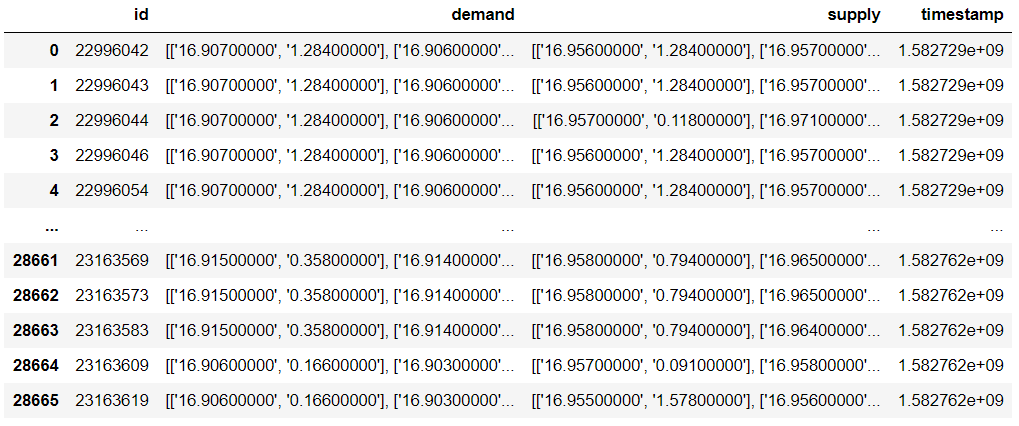
\includegraphics[width=1\textwidth]{images/csv_data.PNG}
	\caption{Ukázka csv souboru jednoho dne dat dvojice kryptoměn}\label{csv_data}
\end{figure}
Order book může mít hloubku až několika stovek objednávek a~poptávek, proto jsem si neukládal jeho celou velikost. Naopak jsem si ukládal pouze pět nejvýhodnějších záznamů. To jsem mohl udělat z~toho důvodu, že arbitrážní příležitost bude vždy nastávat na~nejvýhodnějších nabídkách, protože kdyby nastala na~méně výhodné, tak musela nutně nastat i~na~té nejvýhodnější. 

Hloubku sběru dat z~order booku je možné vybrat libovolnou, vyšší hloubka nezvýší počet výskytu arbitrážních příležitostí, může na~druhou stranu zlepšit absolutní zisk. Hodnoty ve~vyšší hloubce jsou však výrazně méně často využívány (viz koláčový graf \ref{index_distribution}).

Jelikož jsem data potřeboval ukládat neustále a~ne pouze v~konkrétní časové intervaly, tak jsem sběr dat spustil na~cloudové službě AWS - Amazon Web Services. Data jsem kumuloval do~souborů po~jednom dni (v časovém pásmu GMT), protože jsem kvůli omezenému uložišti musel data stahovat a~ukládat i~na~lokální disk.

\subsubsection{Kontrola správnosti dat}
\label{section:kontrola_spravnosti_dat}
Data chodila z~cizího serveru přes websocket a~nebylo stoprocentně zaručené, že budou chodit vždy ve~správném tvaru už jen například v~závislosti na~latenci mezi burzou Binance a~mým serverem. Kvůli tomu bylo nutné zavést některá opatření, aby mi jisté chyby nezkreslily statistiky.

Tento efekt se~objevil, když mi na~několik sledovaných měnových párů začala chodit data po~několik dní (od 18.~2. 2020 až do 3.~3. 2020) opakovaně s~několika sekundovou (až minutovou) časovou prodlevou. Kvůli tomu jsem si napsal program, který mi celé soubory dat zkontroluje, seřadí podle identifikátoru knihy objednávek (order book) a~časového razítka (timestamp) a~následně odstraní duplicity (pro více informací viz kapiola \ref{subsection:cleanup}). 

Tímto kontrolujícím programem jsem zkontroloval všechny soubory a~téměř žádné, až na~pár výjimek (kde byla data duplikovaná), nebyly programem modifikovány, protože data chodila v~korektním formátu.

\subsubsection{Sledované měny a~trojúhelníky}
Na serveru Binance je možné obchodovat s~1320 různými měnami (údaj k~29.~3. 2020), proto jsem si mohl k~obchodování vybrat téměř jakékoliv měny. Z~toho důvodu, že pro mě nebylo reálné sledovat všechny různé dvojice, vybral jsem si ke~sledování následujících 10 kryptoměn: USDT, BTC, LTC, ETH, XRP, BCH, EOS, BNB, TRX, XMR. Toto celkově znamenalo sběr dat týkající se~30 dvojic kryptoměn (obchody mezi některými dvojicemi na~severu Binance nebylo možné provádět).

Celkově je dostupných těchto 30 měnových párů: BCHBNB, BCHBTC, BCHUSDT, BNBBTC, BNBETH, BNBUSDT, BTCUSDT, EOSBNB,  \linebreak EOSBTC, EOSETH, EOSUSDT, ETHBTC, ETHUSDT, LTCBNB, LTCBTC, LTCETH, LTCUSDT, TRXBNB, TRXBTC, TRXETH, TRXUSDT,  \linebreak TRXXRP, XMRBNB, XMRBTC, XMRETH, XMRUSDT, XRPBNB,  \linebreak XRPBTC, XRPETH, XRPUSDT. Všechna tato data nabývala dohromady velikosti v~průměru téměř 1~GB za~den.

Následně zkoumám všech 41 trojúhelníků, které je možné složit, z~těchto měnových párů: BTC/BCH/BNB, BTC/ETH/EOS, BTC/LTC/ETH,  \linebreak ETH/EOS/BNB, USDT/BNB/TRX, USDT/BTC/ETH, USDT/EOS/BNB, USDT/ETH/XRP, XRP/BNB/TRX, BTC/BNB/TRX, BTC/ETH/TRX,  \linebreak BTC/XRP/BNB, ETH/XRP/BNB, USDT/BNB/XMR, USDT/BTC/LTC, USDT/ETH/BNB, USDT/LTC/BNB, BTC/BNB/XMR, BTC/ETH/XMR, BTC/XRP/TRX, ETH/XRP/TRX, USDT/BTC/BCH, USDT/BTC/TRX, USDT/ETH/EOS, USDT/LTC/ETH, BTC/EOS/BNB, BTC/ETH/XRP,  \linebreak ETH/BNB/TRX, LTC/ETH/BNB, USDT/BTC/BNB, USDT/BTC/XMR, USDT/ETH/TRX, USDT/XRP/BNB, BTC/ETH/BNB, BTC/LTC/BNB, ETH/BNB/XMR, USDT/BCH/BNB, USDT/BTC/EOS, USDT/BTC/XRP, USDT/ETH/XMR, USDT/XRP/TRX.
% todo - napsat názvy měn

\section{Zpracování dat}
\subsection{Filtrování surových dat}
V prvním kroku bylo mým cílem pouze vyfiltrovat všechny potenciální arbitrážní příležitosti, které se~na~jednotlivých trojúhelnících objevovaly.

Nejdříve jsem tento filtrovací skript napsal v~jazyce Python. Zde však probíhalo filtrování moc pomalu, řádově několik minut pro provedení jednoho trojúhelníku za~jeden den, což se~po pře násobení počtem trojúhelníků dostalo na~několik hodin denně. Z~toho důvodu jsem výběr jazyka Python přehodnotil a~rozhodl jsem se~využít jazyk C++. V jazyce C++ se~mi podařilo filtrování zrychlit téměř šedesátkrát, tudíž jsem se~dostal z~řádu hodin denně na~řádově minuty.

\subsubsection{Struktura filtrovaných dat}
Vyfiltrovaná data jsem  tentokrát ukládal v~JSON formátu. Tento formát jsem vybral, neboť je zde možné přehledněji strukturovat data (viz ukázka formátu \ref{json_data}).

Na nejnižší úrovni JSON formátu jsem si ukládal tyto informace:
\begin{itemize}
    \item arbitrages\_count -- celé číslo popisující počet nalezených arbitrážních příležitostí v~konkrétním dni,
    \item without\_fees\_count -- celé číslo popisující počet nalezených neefektivit trhu, (kolikrát by se~vyskytla arbitrážní příležitost, kdyby na~burze neexistovaly poplatky), 
    \item all\_count -- celé číslo, které udává kolik celkově proběhlo kontrol na~výskyt arbitrážní příležitosti (neboli počet záznamů order book na~třech \linebreak příslušných měnových párech).
    \item arbitrages\_stats -- pole, ve~kterém jsou uvedeny bližší informace, ke~každé arbitrážní příležitosti. 
    % \todo[]{osobně bych dal ty položky tučně a popis normálně. Koukám, že musím všude u sebe dopsat pomlčky}
\end{itemize}
Co se~týče bližších informací k~jednotlivým arbitrážním příležitostem, tak jsem zachovával následující data:

\begin{itemize}
    \item score -- desetinné číslo popisující teoretický procentuální zisk (bez zahrnutí poplatků),
    \item supply\_gain\_index (demand\_gain\_index) -- pole tří indexů popisující nejlepší kombinaci z~order book k~získání nejvyššího absolutního zisku na~straně trojúhelníku začínajícího nabídkou resp. poptávkou,
    \item supply\_gain (demand\_gain) -- hodnota absolutního zisku hlavní měny v~prvním měnovém páru v~odrážce pairs na~straně trojúhelníku začínajícího nabídkou resp. poptávkou, pokud nedojde žádnému zisku je hodnota ponechána na~0,
    \item time\_delta -- zaznamenává detekovanou dobu výskytu arbitrážní \linebreak příležitosti, 
    \item pairs -- jedná se~o pole o~velikosti 3, na~jehož každé položce je uloženo příslušné identifikační číslo, časový záznam,~typ měnové dvojice a informace o nabídkách a poptávkách ze~čtených csv souborů (viz ukázka csv souboru \ref{csv_data}).
\end{itemize}
\begin{figure}\centering
	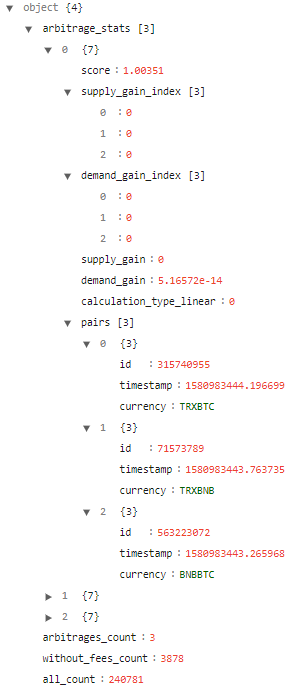
\includegraphics[width=0.6\textwidth]{images/json_data.PNG}
	\caption{Ukázka JSON formátu struktury dat}\label{json_data}
\end{figure}
%\ref{fig:gnuplot-col}
% todo - změnit obrázek na~JSON example
\subsection{Arbitrážní příležitosti}
Ve své práci se~věnuji pouze trojúhelníkovým arbitrážním příležitostem, tedy vždy příležitostem pro 3 odlišné měny. Jelikož mám pro libovolnou obchodovatelnou dvojici kryptoměn (AAA a~BBB) vždy údaj pouze z~jedné strany (poptávka i~nabídka je pouze z~pohledu jedné z~kryptoměn) může docházet v~trojúhelníku k~osmi možnostem uskupení měnových párů. Těchto osm \linebreak možností je však možné přeskupením dostat do~dvou odlišných kombinací.

Tyto dvě kombinace je nutné příslušně vynásobit (resp. vydělit) v~závislosti na~pořadí měn v~měnovém páru. V~trojúhelníku nezáleží na~pořadí, v~jakém jsou jednotlivé hodnoty mezi sebou vynásobeny (vyděleny). Je nutné však vždy v~jednom trojúhelníku zkontrolovat obě strany nákupu a~prodeje.

Dalším krokem v~rámci detekce ideální příležitosti je projití několika dalších nejlepších nabídek (poptávek), v~mém případě do~hloubky pět, a~zjišťovat, jestli není výhodnější provést obchod s~menším procentuálním ziskem, avšak s~vyšším absolutním ziskem. Snažím se~tedy najít takovou možnost, při které dojde k~zobchodování většího množství a~tím vznikne vyšší zisk (viz obrázek \ref{triangle_arbitrage}).

Ve většině případů je i~k~získání největšího absolutního zisku nejvýhodnější využít prvních hodnot v~rámci order book. Celkově je v~mém případě využita první hodnota z~order book ve~více než 80~\% (statistika byla prováděna na~reálných arbitrážních příležitostech získaných v~mé praktické části, celkově bylo vzato v~potaz více než 70~tisíc indexů). Využití dalších indexů v~pořadí je využito o~poznání méně řádově v~jednotkách procent, které se~snižují s~každým dalším indexem (viz koláčový graf \ref{index_distribution}).

K získání úplně nejvyššího absolutního zisku by bylo nutné neobchodovat trojúhelník v hloubce s nejvyšším absolutním ziskem, ale zobchodovat všechny kladné trojúhelníky do sbírané hloubky v pořadí od nejlepšího procentuálního zisku. Takovýto obchod by sice přinesl nejvyšší zisk, ale pro jeho provedení by bylo nutné provést velké množství transakcí, které není většinou reálně možné stihnout.

\begin{figure}\centering
	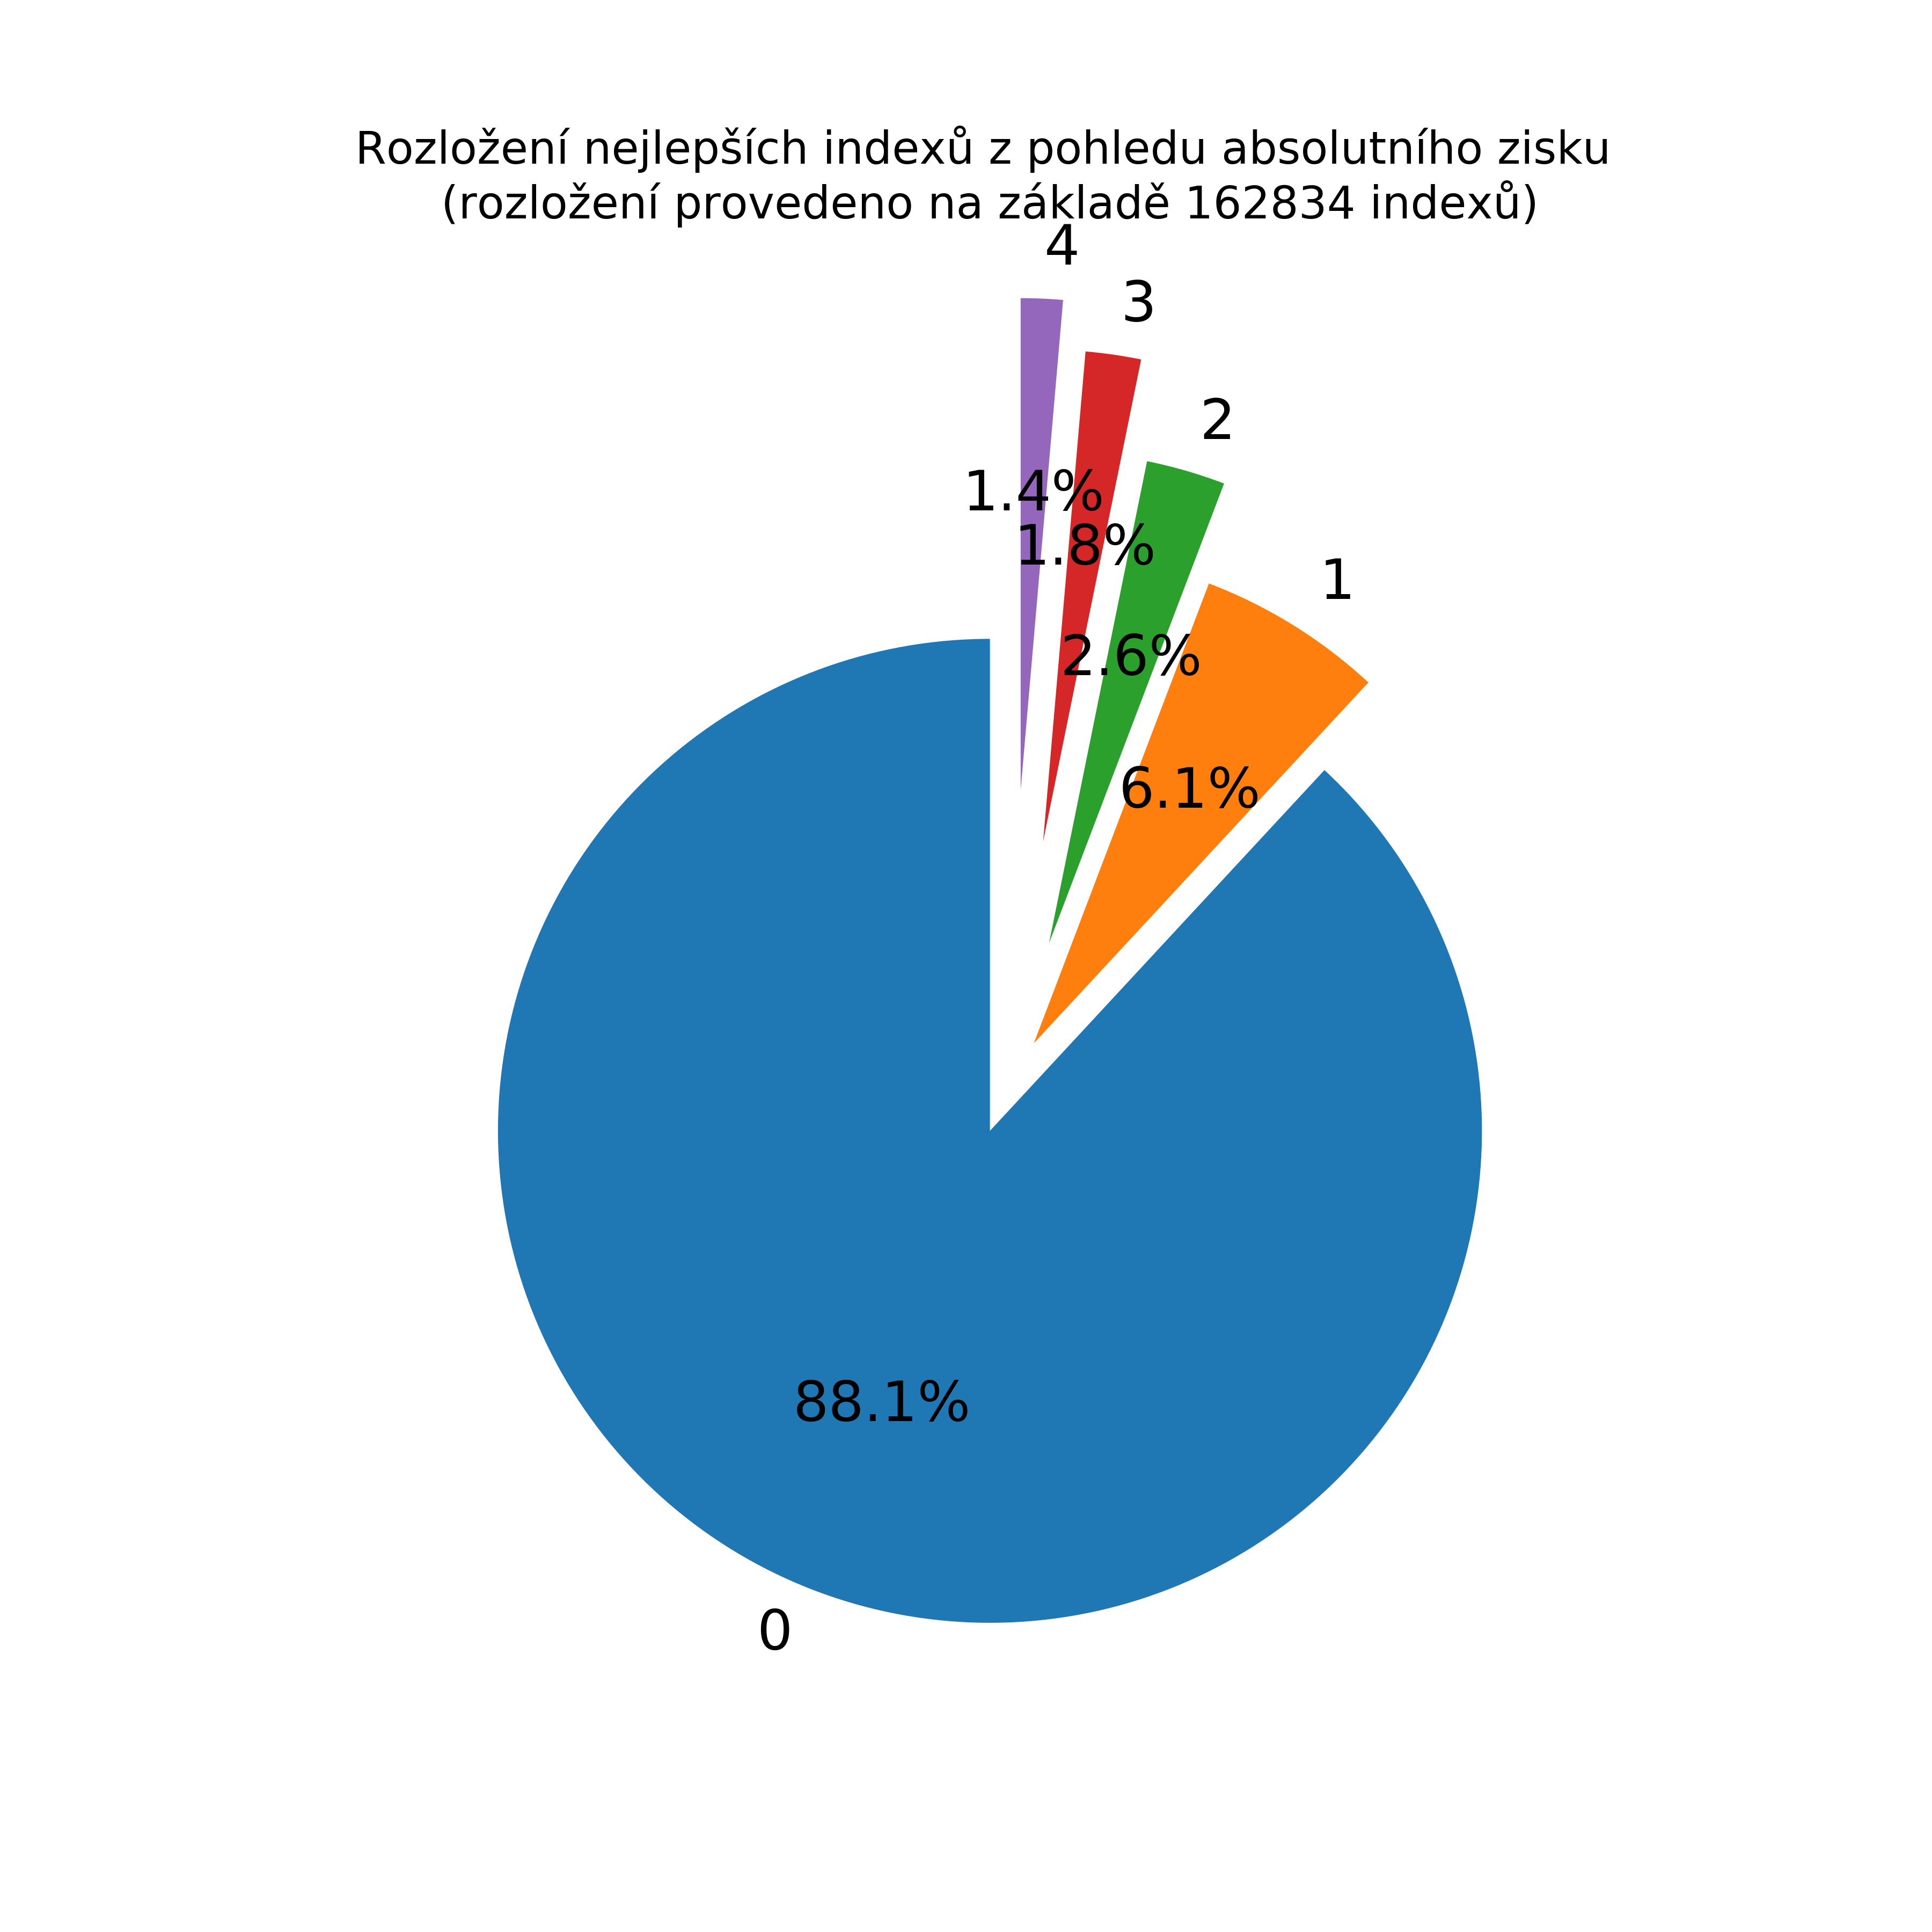
\includegraphics[width=1\textwidth]{images/index_distribution.png}
	\caption{Distribuce indexů obsahující nejlepší hodnoty pro získání nejvyššího absolutního zisku v~rámci arbitrážní příležitosti}\label{index_distribution}
\end{figure}
\subsubsection{Detekce trojúhelníkové arbitrážní příležitosti}
Nechť máme tři odlišné měny \(C_1,C_2,C_3\) a~nechť existují směnné kurzy mezi každou dvojicí měn. Následně definujme \(x_i(t)\) jako výši prodejní ceny (bid) v~čase \(t\) mezi \(C_i\) a~\(C_{i+1}\) za~předpokladu, že \(C_{i+1}\) odpovídá hlavní měně a~\(C_{i}\) odpovídá kótované měně v~uvedeném kurzu. V~opačném případě, kdy \(C_{i}\) je hlavní měna a~\(C_{i+1}\) je měna kótovaná, nastavíme hodnotu \(x_i(t)\) jako převrácenou hodnotu nákupní ceny (ask) v~čase \(t\).

Dále definujme \(f_i\) jako poplatek mezi měnami \(C_i\) a~\(C_{i+1}\), kde pro zjednodušení notace \(C_1 = C_4\).

Následně definujme
\begin{equation}
\label{arbitrage_equation}
    D_{C_1,C_2,C_3}(t) = \prod_i^3\Big(x_i(t)*(1-f_i)\Big) \enspace ,
\end{equation}
jako procentuální efektivitu trojúhelníku v~čase \(t\).

% \todo{prostředí align}

V závislosti na~vztahu mezi \(1\) a~\(D_{C_1,C_2,C_3}(t)\) je možné vyhodnotit, zdali se~jedná o~arbitrážní příležitost. Možnosti jsou následující:
\begin{itemize}
    \item za~předpokladu, že \(D_{C_1,C_2,C_3}(t) < 1\), není detekována arbitrážní  \linebreak příležitost a~při provedení obchodu by došlo ke~ztrátě,
    \item pokud \(D_{C_1,C_2,C_3}(t) > 1\), poté dochází k~detekci arbitrážní příležitosti a~je možné vydělat \( (D_{C_1,C_2,C_3}(t) - 1) * m\), kde \(m\) reprezentuje zobchodované množství,
    \item pokud \(D_{C_1,C_2,C_3}(t) = 1\), pak není nutné trojúhelník obchodovat, protože by nedošlo k~žádnému výdělku.
\end{itemize}

\subsubsection{Reálný příklad arbitrážní příležitosti}
Na obrázku \ref{triangle_arbitrage} je zachycena reálná arbitrážní příležitost na~trojúhelníku USDT/BTC/TRX, která nastala 30.~dubna 2020 v~8:30:29.246  \linebreak středoevropského letního času (čas \(t\) pro výpočet následujícího příkladu). 

\begin{figure}\centering
	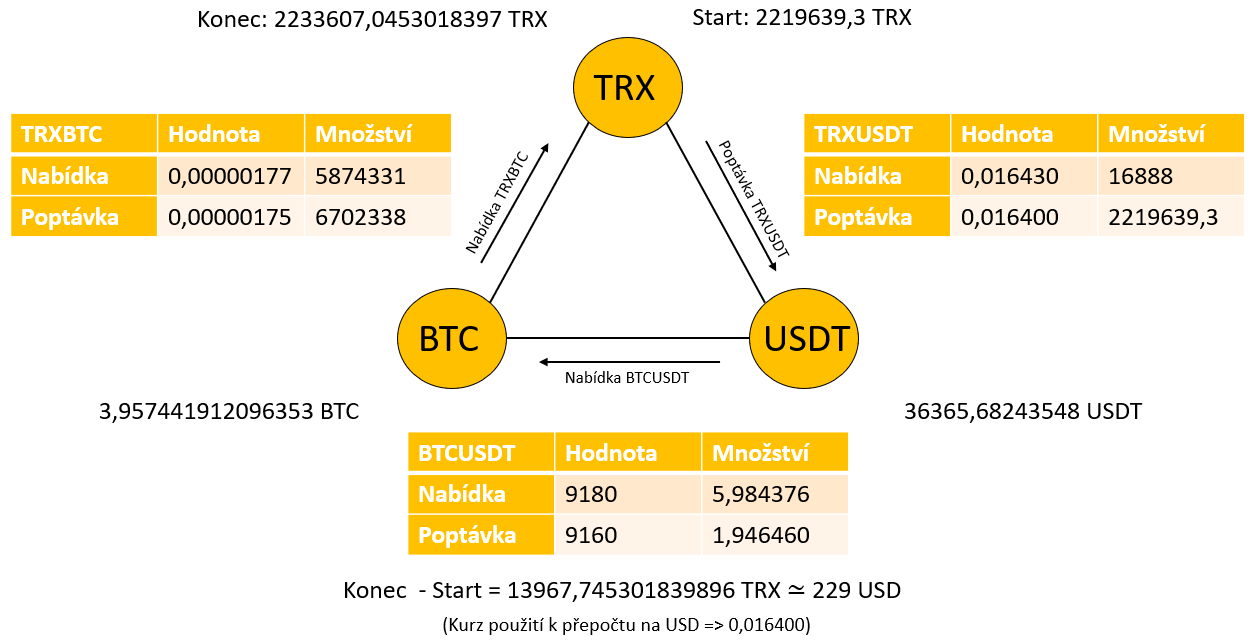
\includegraphics[width=1\textwidth]{images/triangle.png}
	\caption{Trojúhelníková arbitráž}\label{triangle_arbitrage}
\end{figure}

% \begin{equation}
% \label{arbitrage_equation}
%     D_{C_1,C_2,C_3}(t) = \prod_i^3\Big(x_i(t)*(1-f_i)\Big) \enspace ,
% \end{equation}

Na tomto příkladě je počítáno s~poplatky 0,1~\% pro každý měnový pár. po~dosazení do~rovnice \ref{arbitrage_equation} vyjde:

\[D_{USDT,BTC,TRX}(t) = 0,0164 / 9180 / 0,00000177 * (1 - 0,001)^3 = 1,0062928 \]

Nejužší částí tohoto trojúhelníku je množství poptávky na~straně \linebreak~TRXUSDT, proto tuto hodnotu zvolíme jako maximální obchodovatelný objem arbitrážní příležitosti a~vynásobíme upraveným procentuálním ziskem. 
\[(D_{USDT,BTC,TRX}(t) - 1) * m = (1,0062928 - 1) * 2219639,3 = 13967,745\;TRX\]

Na příkladu je vidět, že na~této konkrétní arbitrážní příležitosti bylo možné ~převodu byl využit z~obrázku \ref{triangle_arbitrage} na~straně poptávky na~straně TRXUSDT).

Tato hodnota vypadá velmi zajímavě, je však nutné podotknout, že \linebreak k~vytěžení takovéto arbitrážní příležitosti je nutné zobchodovat objem o~velikosti 2~219~639,3~TRX odpovídajících asi 36~402 americkým dolarům. 

\subsubsection{Reálná detekce arbitrážní příležitosti}
Ve své praktické části detekuji arbitrážní příležitosti stejným způsobem, jaký je popsán v~předchozí sekci. Protože se~však na~data koukám později a~analýzu provádím na~historických datech, je nutné určit, co považuji za~novou arbitrážní příležitost.

Problém může nastat, pokud se~objeví arbitrážní příležitost, která není vytěžena nebo je pouze částečně vytěžena do~příchodu dalšího záznamu (order book). S~takovýmto efektem nakládám tím způsobem, že pokud se~vyskytne několik stejných arbitrážní příležitostí po~sobě, považuji je za~jednu a~pouze zvětšuji dobu trvání výskytu dané arbitrážní příležitosti.

Je nutné ještě zadefinovat, co považuji za~stejnou arbitrážní příležitost. Jako stejnou arbitrážní příležitost považuji takovou, která má stejné právě 2~časová razítka (timestamp) a~stejný procentuální zisk. 

Absolutní zisky neporovnávám z~toho důvodu, že může dojít pouze ke~změně v~obchodovatelnému objemu arbitrážní příležitosti. Tudíž kdybych tyto menší arbitrážní příležitosti detekoval jako nové, došlo by k~duplikování stejných hodnot na~jiných arbitrážních příležitostech. Další obrácenou možností je to, že by někdo vytvořil podobnou nabídku a~tím zvýšil potenciální zisk to by však bylo moc složité na~detekci, a~proto se~tomu ve~své práci nevěnuji. 

\subsubsection{Příklad výskytu a jeho detekce}
Neboť je detekce arbitrážních příležitostí prováděna na historických datech a neboť je k~jednotlivým order book záznamům přidáváno časové razítko až po~přečtení dat, považuji daný order book za aktuální až do příchodu nadcházejícího záznamu na stejném měnovém páru. Proto je nutné při inicializaci detekce příležitostí přečíst na každém měnovém páru alespoň dva záznamy. Přičemž je nutné v programu dohlédnout na to, aby bylo přečteno dostatek záznamů na to, aby se intervaly počítaných měnových párů překrývaly. 

Program vyhledávající pozitivní arbitrážní příležitosti iteruje postupně všemi třemi soubory měnových párů následujícím algoritmem. 

Předpokládám, že se nejedná o začátek programu, proto mám již načtený trojúhelník, který byl zkontrolován na výskyt arbitrážní příležitosti. Dále mám načtené hodnoty nadcházejících záznamů. V dalším kroku je vyměněna ta hrana trojúhelníku, která má z~dopředu načtených hodnot nejnižší timestamp. Takto je zajištěno, že se intervaly překrývají. 

\begin{table}\centering
\caption{Příklad k postupné kontrole na pozitivní arbitrážní příležitosti}
\label{timestamp_example}
\begin{tabular}{|| l | r | r | r ||}\hline Měnový pár & 1. hodnota & 2. hodnota & 3. hodnota\\ [0.5ex]
 \hline
 \hline A & 0,01 & 0,03 & 0,06\\ 
 \hline B & 0,00 & 0,02 & 0,07\\ 
 \hline C & 0,00 & 0,04 & 0,05\\ 
 \hline
\end{tabular}
\end{table}

Trojúhelníky jsou vybírány a kontrolovány následovně (viz tabulka \ref{timestamp_example}), T(t) značí čas začátku nového trojúhelníku (A, B, C značí různé měnové páry):
\begin{itemize}
    \item T(0,01) = A1, B1, C1,
    \item T(0,02) = A1, B2, C1 (výskyt),
    \item T(0,03) = A2, B2, C1,
    \item T(0,04) = A2, B2, C2 (zánik),
    \item T(0,05) = A2, B2, C3,
    \item T(0,06) = A3, B2, C3,
    \item T(0,07) = A3, B3, C3,
\end{itemize}

Řekněme že se s příchodem nové hodnoty na měnové páru B v čase T(0,02) objeví nová pozitivní arbitrážní příležitost. Tato příležitost zanikne v čase T(0,04) se změnou hodnoty na měnovém páru C. Arbitrážní příležitost tedy v~tomto případě stihla zmizet dříve, než byl přečten nový order book na~měnovém páru B, který způsobil výskyt pozitivní příležitosti. 
\subsection{Kontrola dat}
\subsubsection{Kontrola korektnosti záznamů}
\label{section:kontrola_korektnosti_zaznamu}
V rámci procházení souborů je nutné kontrolovat, zdali jsou záznamy korektní. Data jsou kontrolována na správnost typů a správnost požadovaného formátu. Je nutné však ještě kontrolovat záznamy na správnost pořadí.

Záznamy jsou kontrolovány na souslednost identifikačních čísel. Dále jsou kontrolována časová razítka (timestamp) a to tak, že se porovnává rozdíl mezi aktuálním a následujícím záznamem. Jako korektní je považován monotónní záznam s adekvátní časovou prodlevou. 

Adekvátní časovou prodlevu je nutné určit pro každý měnový pár zvlášť, neboť jsou nějaké měnové páry vytíženější než jiné. Adekvátní časové prodlevy jsem volil následujícím způsobem:

\begin{enumerate}
    \item vybral jsem dny, které měly konzistentní data (konkrétně dny od 10.~4. 2020 až do 17.~5. 2020),
    \item na těchto datech jsem spočítal percentil 99,9 pro každý den a pro každý měnový pár zvlášť,
    \item zvolil jsem medián ze spočítaných percentilů přes tyto dny (viz tabulka časových prodlev \ref{tolerances}).
    \item tento medián jsem vynásobil konstantou 1,1 a tím určil adekvátní časovou prodlevu.
\end{enumerate}

Byl zvolen percentil 99,9, neboť data byla konzistentní a nedocházelo k~velkým výkyvům. Medián byl vybrán, protože jsem nechtěl, aby případný větší výkyv v některém dni nerozházel data. Konstanta 1,1 byla vybrána, aby došlo k zahození menší části dat a stále byly detekovány velké výkyvy.

Konstanta 1,1 byla zaměněna za konstantu 1,5 pro takové výskyty, kdy na~sebe přímo navazovala identifikační čísla po sobě jdoucích záznamů. Identifikační čísla obchodů na sebe vždy nenavazovala, byla však vždy seřazená. 

\begin{table}\centering
\caption{Hodnoty adekvátní časové prodlevy pro jednotlivé měnové páry}
\label{tolerances}
\begin{tabular}{|| l | r ||}\hline Měnový pár & Denní medián percentilů (99,9) časových prodlev (s)\\ [0.5ex]
 \hline
  \hline BCH/BNB & 15,38 \\
  \hline BCH/BTC & 1,78 \\
  \hline BCH/USDT & 1,06 \\
  \hline BNB/BTC & 2,07 \\
  \hline BNB/ETH & 4,91 \\
  \hline BNB/USDT & 1,53 \\
  \hline BTC/USDT & 1,04 \\
  \hline EOS/BNB & 11,83 \\
  \hline EOS/BTC & 3,17 \\
  \hline EOS/ETH & 5,86 \\
  \hline EOS/USDT & 1,08 \\
  \hline ETH/BTC & 1,08 \\
  \hline ETH/USDT & 1,04 \\
  \hline LTC/BNB & 19,04 \\
  \hline LTC/BTC & 2,53 \\
  \hline LTC/ETH & 6,28 \\
  \hline LTC/USDT & 1,32 \\
  \hline TRX/BNB & 14,25 \\
  \hline TRX/BTC & 3,20 \\
  \hline TRX/ETH & 5,47 \\
  \hline TRX/USDT & 2,35 \\
  \hline TRX/XRP & 20,31 \\
  \hline XMR/BNB & 29,27 \\
  \hline XMR/BTC & 5,12 \\
  \hline XMR/ETH & 12,86 \\
  \hline XMR/USDT & 2,98 \\
  \hline XRP/BNB & 14,45 \\
  \hline XRP/BTC & 2.,68 \\
  \hline XRP/ETH & 4,03 \\
  \hline XRP/USDT & 1,12 \\
  \hline
\end{tabular}
\end{table}

\subsubsection{Kontrola pozitivních arbitrážních příležitostí}
\label{section:kontrola_pozitivnich_arbitraznich_prilezitosti}
V předchozí sekci byla zmíněna problematika správnosti záznamů v rámci jednotlivých měnových párů, je však nutné kontrolovat i nalezené arbitrážní příležitosti na správnost časového překrytí intervalů. 

Arbitrážní příležitosti jsou kontrolovány následovně. Je spočítán rozdíl nejvzdálenějších časových razítek s~nejvyšší adekvátní časovou prodlevou ze zúčastněných párů. Pokud je tato hodnota záporná je považována arbitrážní příležitost za validní.

\subsubsection{Problém s duplicitami}
V datech (od 18.~2. 2020 do 3.~3. 2020) se objevily zmiňované duplicity z~kapitoly \ref{section:kontrola_spravnosti_dat}. Duplicity se mi podařilo odstranit kompletně. Vznikl však problém, že v nějakých časových okamžicích byla data uložena rozházeně podle identifikačních čísel (není zřejmé, jestli byla chyba na mojí straně nebo na~straně serveru Binance).

Tyto chyby následně způsobily, že časová razítka nebyla monotónně rostoucí. Těchto chyb se objevovalo na některých měnových párech několik stovek až několik tisíc za den (většina souborů měla okolo 60 až 100 tisíc záznamů). 

S poškozenými soubory se naskytly dvě možnosti:
\begin{enumerate}
    \item zahodit několikadenní data,
    \item přizpůsobit program, tak aby ignoroval chyby.
\end{enumerate}

Rozhodl jsem se pro druhou možnost, tedy přizpůsobit program chybám. Při výskytu chyby v monotonii jsem restartoval počítací algoritmu a začal jsem znovu s dalšími správnými hodnotami. Správné hodnoty byly vyhodnocovány na základě algoritmu z předchozích sekcí \ref{section:kontrola_korektnosti_zaznamu} a \ref{section:kontrola_pozitivnich_arbitraznich_prilezitosti}.

V datech byla celkově přeskakována poškozená místa v rámci programu, výpočty na výskyt trojúhelníkových arbitrážních příležitostí byly prováděny na korektních částech záznamů. Celkově jsem tedy výběrem možnosti přizpůsobení programu přišel o několik procent záznamů, kde se mohly vyskytovat arbitrážní příležitosti, nepřišel jsem však o všechny záznamy. Upraveným algoritmem by neměly být detekovány nereálné arbitrážní příležitosti. V rámci těchto několika dní se neobjevily žádné větší výkyvy v počtu arbitrážních příležitostí (viz grafy \ref{occurence_correlation} a \ref{occurences}), proto se dovoluji tvrdit, že se podařilo provést analýzu dat i na~částečně poškozených datech.

\section{Struktura modulů praktické části}
Celkově je moje praktická část rozdělena do čtyř na sobě nezávislých modulů, kterými jsou sběr dat, vyčištění dat, selekce trojúhelníků a statistika na trojúhelnících. Neboť je každý modul odlišný ve svém chování, je důležité zmínit některé jejich důležité vlastnosti.

\subsection{Sběr dat}
Sběr dat je implementován jako spustitelný soubor v jazyce Python 3. Tento program stahuje data z burzy Binance přes websocket a ukládá data ve formě order book do souborů po jednotlivých měnových párech a jednotlivých dnech.

Dny jsou rozděleny na základě časové zóny UTC. Univerzální zóna UTC byla zvolena, protože sbírám data ze světové burzy. 

Ke sběru dat je napsaná manuálová stránka vysvětlující jeho funkcionalitu a spouštění a je součástí přílohy (ve stejném adresáři jako program samotný).

\subsection{Čištění dat}
\label{subsection:cleanup}
Program na čištění dat je stejně jako program pro sběr dat napsaný v jazyce Python 3 a~i~on má svou manuálovou stránku s~bližšími informacemi ohledně funkcionality a~ spouštění zahrnutou v příloze. 

Program čištění dat není nutné spouštět na data sebraná z burzy, je to však doporučené, protože data chodí ze vzdáleného serveru přes websocket a občas se v datech vyskytly chyby (například s duplikováním některých záznamů), které program odstraní.

\subsection{Selekce trojúhelníků}
Program na selekci pozitivních trojúhelníků je jako jediná část kódu z důvodu rychlosti napsaná v jazyce C++ Program je možné spouštět na více vláknech. Opět je k němu napsaná manuálová stránka zahrnutá v příloze. 

Selekce trojúhelníků bere data ve formátu csv (viz obrázek \ref{csv_data}) a hledá na~nich pozitivní trojúhelníky (se zahrnutím poplatků burzy), které ukládá opět po dnech a po jednotlivých trojúhelnících ve formátu JSON (viz ukázka dat \ref{json_data}).

\subsection{Statistiky na trojúhelnících}
Poslední část zaobírající se analýzou trojúhelníků je napsaná opět v~jazyce Python 3 avšak ve formě Jupyter notebooku. Tento formát byl zvolen z toho důvodu, že se jedná o přehledný způsob zobrazení grafů a tabulek včetně jejich generujícího kódu. Velkou část kódu totiž tvoří části vykreslující grafy, které se dají jednoduše upravit a vygenerovat podobné grafy.

V této části jsou vytvořené dvě hlavní třídy starající se o přehledné uložení dat, které jsou zdokumentovány v kódu. K Jupyter notebooku neexistuje manuálová stránky, poněvadž jsou jednotlivé kusy kódu okomentovány pomocí jazyka Markdown v rámci Jupyter notebooku. Popis výstupů z Jupyter notebooku je možný najít v poslední kapitole \ref{chapter:analyza_dat}.



\chapter{Analýza dat}
\label{chapter:analyza_dat}
V této kapitole se~věnuji analýze  reálných dat s~pomocí vlastních grafů. Data jsou vyhodnocena na~základě více než dvou měsíční sbírky dat.

\section{Selekce nejlepších trojúhelníků}
V této sekci se~zabývám selekcí těch nejlepších trojúhelníků vzhledem \linebreak k~nejčastějším výskytům arbitrážních příležitostí, největších potenciálních \linebreak zisků. Tato část je nutná z~toho důvodu, že celkově pozoruji 41 odlišných trojúhelníků a~velké části z~nich není nutné se~věnovat, protože nejsou z~pohledu vytěžování arbitrážních příležitostí vůbec zajímavé.

\subsection{Základní statistiky trojúhelníků}
V této podkapitole se~úzce věnuji nejzákladnějším statistikám jednotlivých trojúhelníků a~diskutuji nad tím, jakým se~vyplatí se~věnovat podrobně \linebreak v~dalších částech této kapitoly.

Nejdůležitějšími faktory jsou: 
\begin{itemize}
    \item jak často se~pozitivní arbitrážní příležitosti vyskytují,
    \item jak dlouho průměrně trvají, jak velká pravděpodobnost na~včasné \linebreak vytěžení reálně existuje,
    \item kolik je v~průměru možné vydělat na~úspěšném vytěžení jednotlivé arbitrážní příležitosti,
    \item k~jak velkému potenciálnímu zisku došlo.
\end{itemize}
Jak je možné vidět v~tabulce \ref{table_averages}, tak průměrný počet pozitivních arbitrážních příležitostí se~pro jednotlivé trojúhelníky hodně liší, pohybuje se od~ani ne jednotek denně až po~několik desítek denně. V~případě trojúhelníku  \linebreak USDT/XRP/TRX je tomu nejvíce a~jedná se~v~průměru o~více než 30 pozitivních arbitrážních příležitostí denně. Průměrná neefektivita arbitrážní příležitosti (jedná se~o hodnotu procentuálního zisku se zahrnutím poplatků) dosahuje hodnot promile pouze u trojúhelníků USDT/BCH/BNB \linebreak a USDT/ETH/BNB, u všech ostatních sledovaných trojúhelníků se hodnota pohybuje v řádu desetin promile.

Vyšší procentuální zisk z~tabulky \ref{table_averages} a~grafu \ref{average_percentage_inefficiency} nemusí nutně znamenat vysoký reálný zisk. V~tabulce \ref{table_gains} jsou uvedeny průměrné denní potenciální zisky, jak v~hodnotách jedné z~kryptoměn příslušného trojúhelníku, tak v~hodnotách přepočtených na~americké dolary (podle tabulky kurzů \ref{table_rates}) kvůli lepšího porovnání. V~tabulce potenciálních zisků \ref{table_gains} je vidět, že se~hodnoty liší mezi jednotlivými trojúhelníky znatelněji, než v~tabulce průměrných počtů arbitrážních příležitostí v~tabulce \ref{table_averages}. Průměrné denní potenciální zisky zde kolísají od~hodnot blízkých nule až po~hodnoty desítek až stovek amerických dolarů (údaje jsou nechány v~exponenciálním tvaru, neboť rozdíly mezi nejmenšími a~nejvyššími hodnotami jsou až 6 řádů). 

% todo -- change exp to float

% \hline
% Nazev & Prumerny denni pocet & \vtop{\hbox{\strut Prumerna}\hbox{\strut neefektivita}}\\ [0.5ex]
% \hline 

\begin{table}\centering
\caption{Porovnání denních průměrů a průměrné denní \% neefektivity}
\label{table_averages}
\begin{tabular}{|| l | r | r ||}\hline Trojúhelník & Průměrný denní počet & Průměrná \% neefektivita\\
 \hline\hline BTC/BCH/BNB & 1,9655 & 1,0003\\ 
 \hline BTC/BNB/TRX & 0,5667 & 1,0001\\ 
 \hline BTC/BNB/XMR & 2,8966 & 1,0002\\ 
 \hline BTC/EOS/BNB & 0,8333 & 1,0001\\ 
 \hline BTC/ETH/BNB & 1,0833 & 1,0003\\ 
 \hline BTC/ETH/EOS & 0,7586 & 1,0001\\ 
 \hline BTC/ETH/TRX & 2,1264 & 1,0002\\ 
 \hline BTC/ETH/XMR & 8,1529 & 1,0003\\ 
 \hline BTC/ETH/XRP & 5,1609 & 1,0003\\ 
 \hline BTC/LTC/BNB & 0,8667 & 1,0002\\ 
 \hline BTC/LTC/ETH & 3,9540 & 1,0001\\ 
 \hline BTC/XRP/BNB & 1,2667 & 1,0002\\ 
 \hline BTC/XRP/TRX & 9,0706 & 1,0003\\ 
 \hline ETH/BNB/TRX & 0,6500 & 1,0003\\ 
 \hline ETH/BNB/XMR & 4,6471 & 1,0002\\ 
 \hline ETH/EOS/BNB & 0,3793 & 1,0002\\ 
 \hline ETH/XRP/BNB & 2,4253 & 1,0002\\ 
 \hline ETH/XRP/TRX & 3,8353 & 1,0001\\ 
 \hline LTC/ETH/BNB & 2,8736 & 1,0003\\ 
 \hline USDT/BCH/BNB & 19,3765 & 1,0010\\ 
 \hline USDT/BNB/TRX & 3,5500 & 1,0006\\ 
 \hline USDT/BNB/XMR & 28,9412 & 1,0007\\ 
 \hline USDT/BTC/BCH & 4,6333 & 1,0008\\ 
 \hline USDT/BTC/BNB & 7,0167 & 1,0007\\ 
 \hline USDT/BTC/EOS & 13,3678 & 1,0006\\ 
 \hline USDT/BTC/ETH & 3,6833 & 1,0006\\ 
 \hline USDT/BTC/LTC & 12,9080 & 1,0005\\ 
 \hline USDT/BTC/TRX & 6,3218 & 1,0006\\ 
 \hline USDT/BTC/XMR & 20,4138 & 1,0007\\ 
 \hline USDT/BTC/XRP & 14,4023 & 1,0005\\ 
 \hline USDT/EOS/BNB & 18,2299 & 1,0007\\ 
 \hline USDT/ETH/BNB & 4,8500 & 1,0010\\ 
 \hline USDT/ETH/EOS & 2,8966 & 1,0008\\ 
 \hline USDT/ETH/TRX & 2,9500 & 1,0010\\ 
 \hline USDT/ETH/XMR & 2,6724 & 1,0008\\ 
 \hline USDT/ETH/XRP & 3,6500 & 1,0007\\ 
 \hline USDT/LTC/BNB & 17,7011 & 1,0007\\ 
 \hline USDT/LTC/ETH & 2,4167 & 1,0008\\ 
 \hline USDT/XRP/BNB & 12,8621 & 1,0007\\ 
 \hline USDT/XRP/TRX & 30,9529 & 1,0004\\ 
 \hline XRP/BNB/TRX & 1,1724 & 1,0001\\ 
 \hline
\end{tabular}
\end{table}

\begin{figure}\centering
	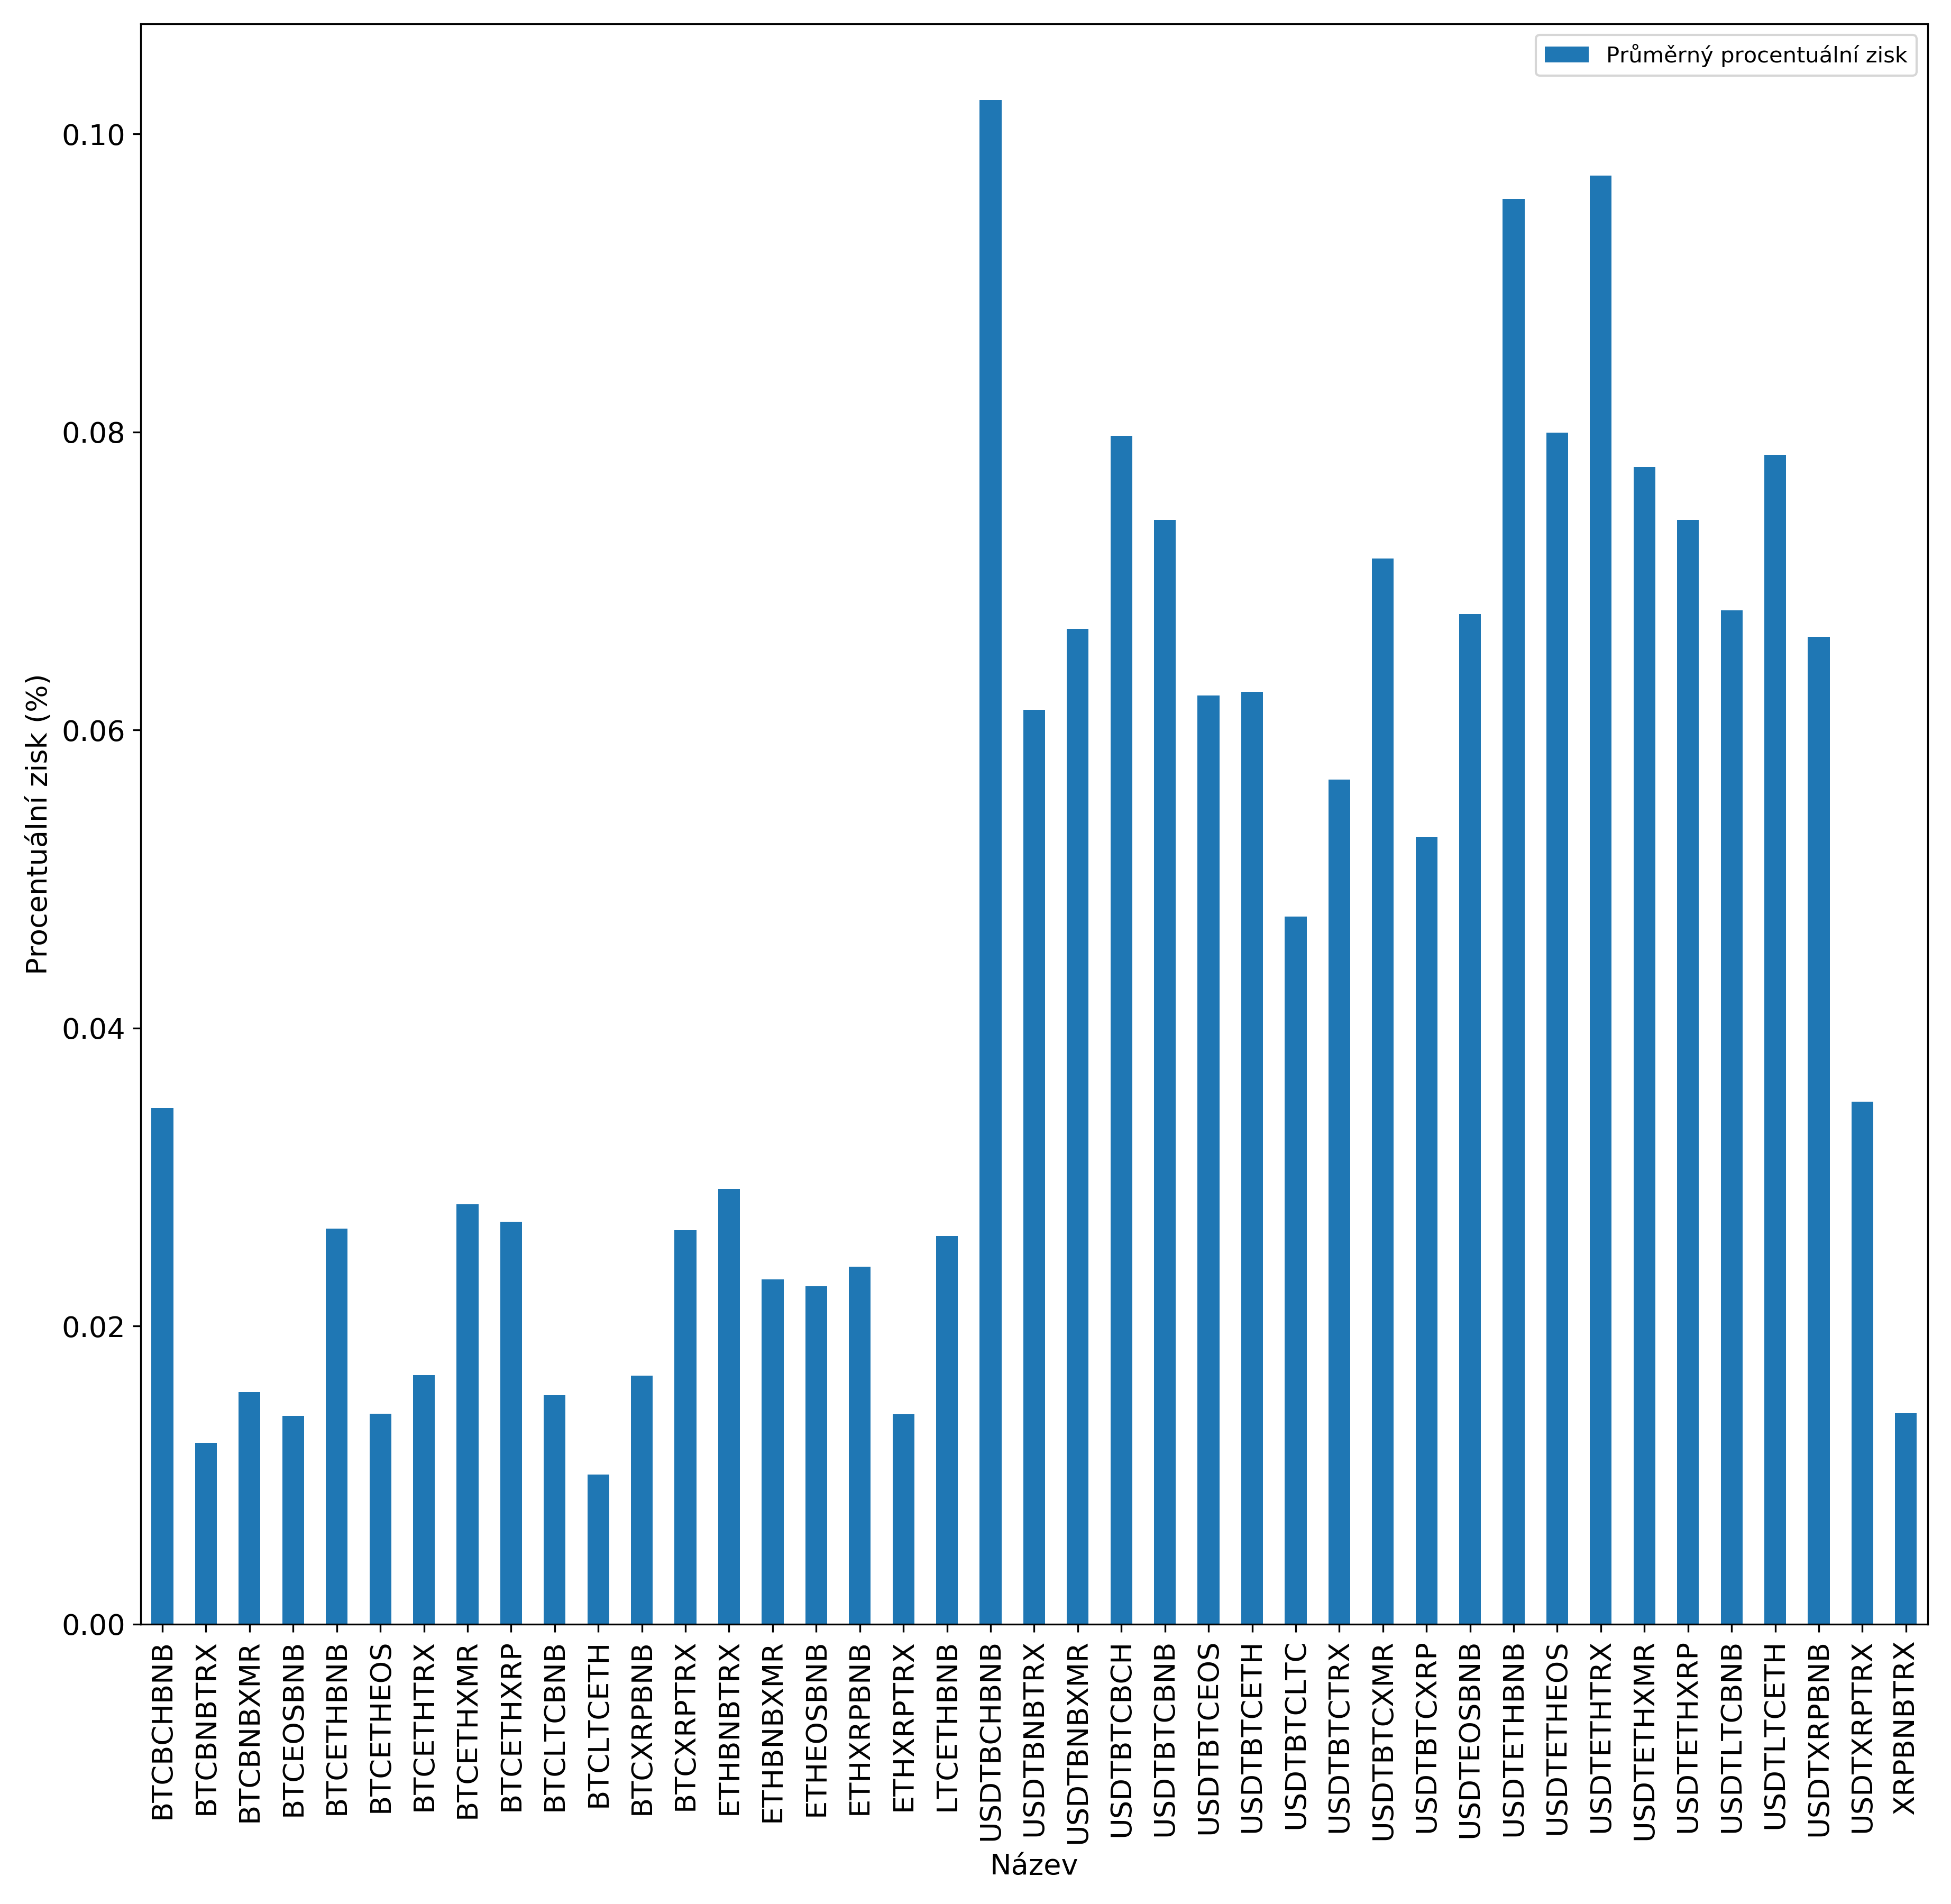
\includegraphics[width=1\textwidth]{images/average_percentage_inefficiency.png}
	\caption{Celkový průměr procentuální neefektivity jednotlivých trojúhelníků (se zahrnutím poplatků)}\label{average_percentage_inefficiency}
\end{figure}

\begin{table}\centering
\caption{Potenciální výnosy na jednotlivých trojúhelnících}
\label{table_gains}
\begin{tabular}{|| l | r | r ||}\hline Trojúhelník & Denní neefektivita & Denní neefektivita (USD)\\
 \hline\hline BTC/BCH/BNB & 0,004686 BCH & 1,044816\\ 
 \hline BTC/BNB/TRX & 37,669655 TRX & 0,474525\\ 
 \hline BTC/BNB/XMR & 0,004210 XMR & 0,224689\\ 
 \hline BTC/EOS/BNB & 0,027397 EOS & 0,066850\\ 
 \hline BTC/ETH/BNB & 0,089227 BNB & 1,385699\\ 
 \hline BTC/ETH/EOS & 0,131114 EOS & 0,319919\\ 
 \hline BTC/ETH/TRX & 194,088264 TRX & 2,444930\\ 
 \hline BTC/ETH/XMR & 0,018077 XMR & 0,964752\\ 
 \hline BTC/ETH/XRP & 18,530255 XRP & 3,445979\\ 
 \hline BTC/LTC/BNB & 0,005206 LTC & 0,213432\\ 
 \hline BTC/LTC/ETH & 0,024868 LTC & 1,019591\\ 
 \hline BTC/XRP/BNB & 5,701600 XRP & 1,060298\\ 
 \hline BTC/XRP/TRX & 312,897841 TRX & 3,941574\\ 
 \hline ETH/BNB/TRX & 43,673148 TRX & 0,550151\\ 
 \hline ETH/BNB/XMR & 0,043821 XMR & 2,338744\\ 
 \hline ETH/EOS/BNB & 0,054539 EOS & 0,133074\\ 
 \hline ETH/XRP/BNB & 2,743739 XRP & 0,510239\\ 
 \hline ETH/XRP/TRX & 25,129313 TRX & 0,316554\\ 
 \hline LTC/ETH/BNB & 0,011626 LTC & 0,476660\\ 
 \hline USDT/BCH/BNB & 0,381556 BCH & 85,079456\\ 
 \hline USDT/BNB/TRX & 147,677652 TRX & 1,860295\\ 
 \hline USDT/BNB/XMR & 2,072639 XMR & 110,616732\\ 
 \hline USDT/BTC/BCH & 0,080214 BCH & 17,886043\\ 
 \hline USDT/BTC/BNB & 1,335634 BNB & 20,742392\\ 
 \hline USDT/BTC/EOS & 48,942284 EOS & 119,419172\\ 
 \hline USDT/BTC/ETH & 0,127004 ETH & 19,901603\\ 
 \hline USDT/BTC/LTC & 2,433303 LTC & 99,765406\\ 
 \hline USDT/BTC/TRX & 8341,144951 TRX & 105,073403\\ 
 \hline USDT/BTC/XMR & 0,996903 XMR & 53,204728\\ 
 \hline USDT/BTC/XRP & 567,311008 XRP & 105,499992\\ 
 \hline USDT/EOS/BNB & 73,154081 EOS & 178,495958\\ 
 \hline USDT/ETH/BNB & 0,365623 BNB & 5,678119\\ 
 \hline USDT/ETH/EOS & 1,768986 EOS & 4,316326\\ 
 \hline USDT/ETH/TRX & 568,958881 TRX & 7,167175\\ 
 \hline USDT/ETH/XMR & 0,048328 XMR & 2,579268\\ 
 \hline USDT/ETH/XRP & 20,859336 XRP & 3,879106\\ 
 \hline USDT/LTC/BNB & 2,132622 LTC & 87,437498\\ 
 \hline USDT/LTC/ETH & 0,101542 LTC & 4,163237\\ 
 \hline USDT/XRP/BNB & 564,157920 XRP & 104,913628\\ 
 \hline USDT/XRP/TRX & 1910,791414 TRX & 24,070239\\ 
 \hline XRP/BNB/TRX & 4,881886 TRX & 0,061497\\ 
 \hline
\end{tabular}
\end{table}

\begin{table}\centering
\caption{Kurzy využité k~přepočetu na~americké dolary (údaj z~burzy Binance ze~dne 13.4.2020)}
\label{table_rates}
\begin{tabular}{|| l | r ||}
\hline Kryptoměna & Kurz na~USD \\ 
\hline\hline BTC & 6837,51 \\ 
\hline LTC & 41 \\ 
\hline ETH & 156,7 \\ 
\hline XRP & 0,185965 \\ 
\hline USDT & 1 \\ 
\hline BCH & 222,98 \\ 
\hline BNB & 15,53 \\ 
\hline EOS & 2,44 \\ 
\hline XMR & 53,37 \\ 
\hline TRX & 0,012597 \\ 
\hline
\end{tabular}
\end{table}


\section{Korelace mezi výskytem arbitrážních příležitostí a~vnějšími jevy}
V této sekci se~zabývám tím, jaké vnější jevy mohou mít na~výskyt arbitrážních příležitostí vliv a~jak moc s~výskytem korelují nebo nekorelují. Je nutné podotknout, že nějaké vztahy nemusí být úplně vypovídající, protože korelace jsou prováděny pouze na~datech o~velikosti dvou až tří měsíců.

\subsection{Závislost na~dni v~týdnu}
Z grafu \ref{weekday_distribution} je možné vidět, že se~arbitrážní příležitosti vyskytovaly nejvíce v~pondělí, v~úterý a v neděli. Na~druhou stranu při pohledu na~graf \ref{occurences} je jasně vidět, že se ve~výskytu arbitrážních příležitostí nevyskytuje žádný periodický vzor, který by se~opakoval po~každých sedmi dnech. Graf je velice plochý s~pár výkyvy, které naprosto převáží všechny ostatní výskyty.

Proto si dovoluji tvrdit, že z~mých dat není zřejmá žádná korelace mezi výskytem arbitrážních příležitostí a~dnem v~týdnu. Nevyvracím však možnost, že se~nějaká vyskytovat může. Velké výkyvy ve~výskytu arbitráží ovlivňují data natolik, že ostatní hodnoty mají téměř nulový význam.

\begin{figure}\centering
	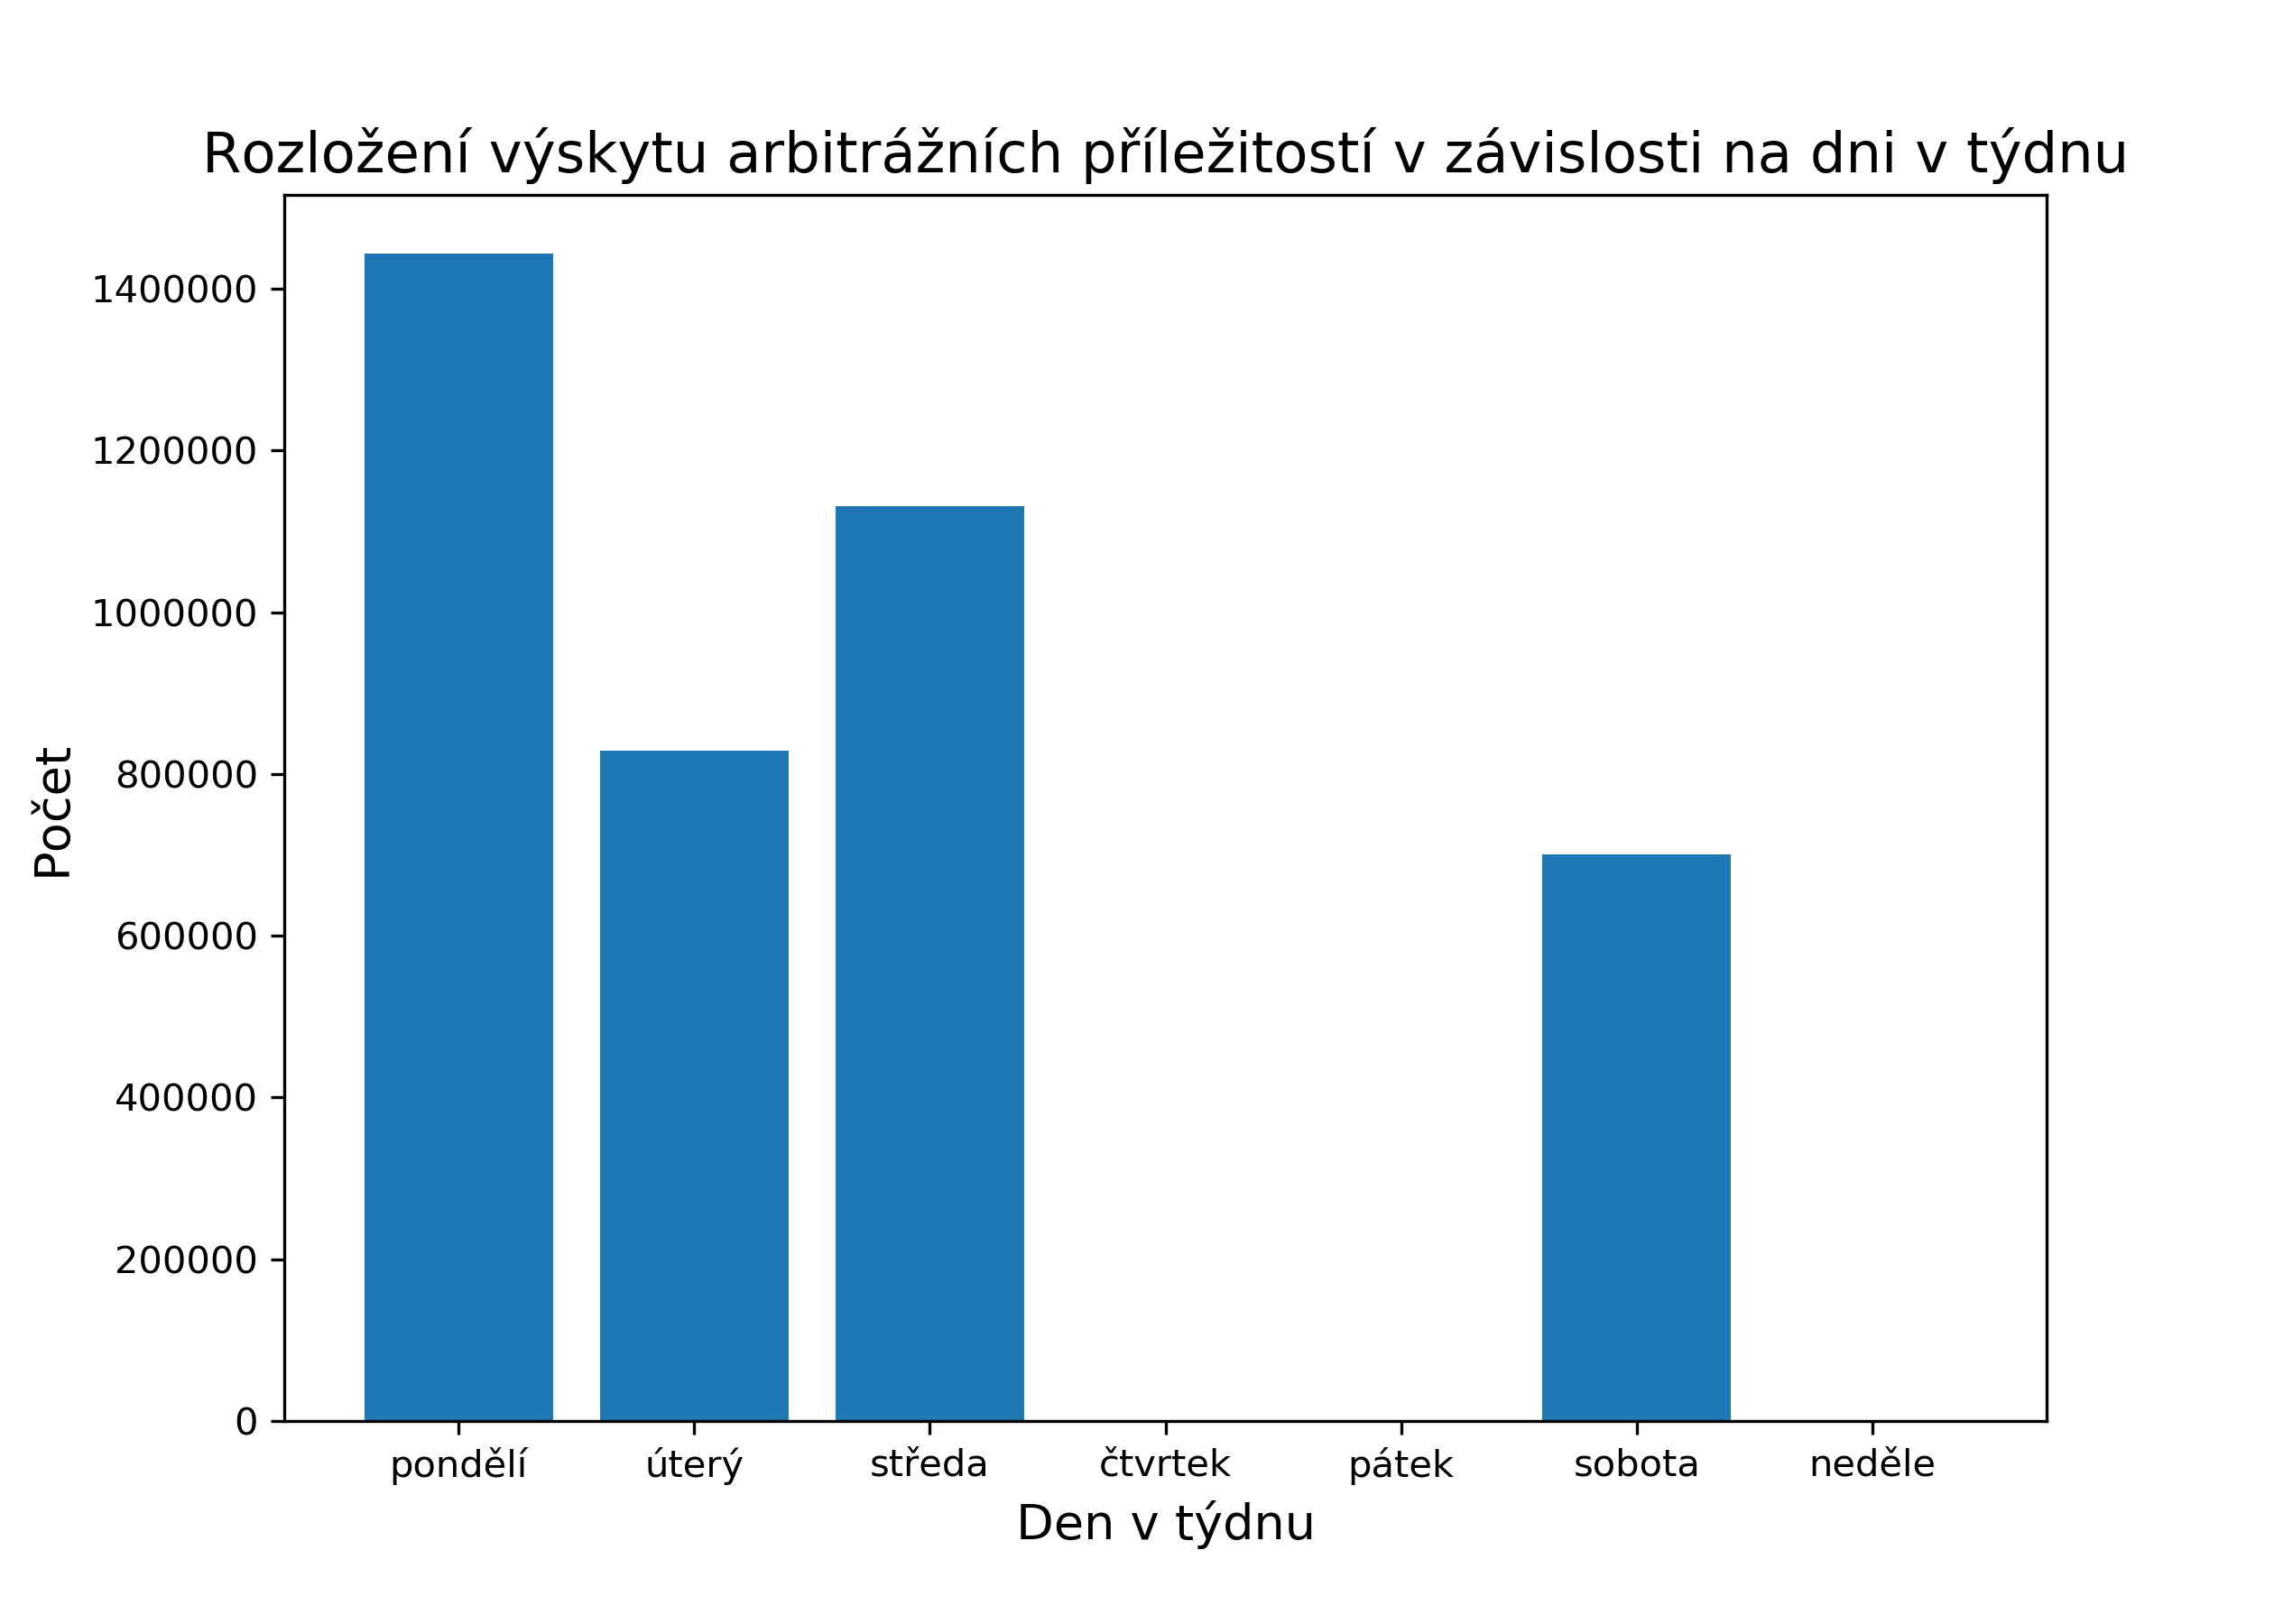
\includegraphics[width=1\textwidth]{images/weekday_distribution.png}
	\caption{Rozložení arbitrážních příležitostí v~závislosti na~dni v~týdnu }\label{weekday_distribution}
\end{figure}
\begin{figure}\centering
	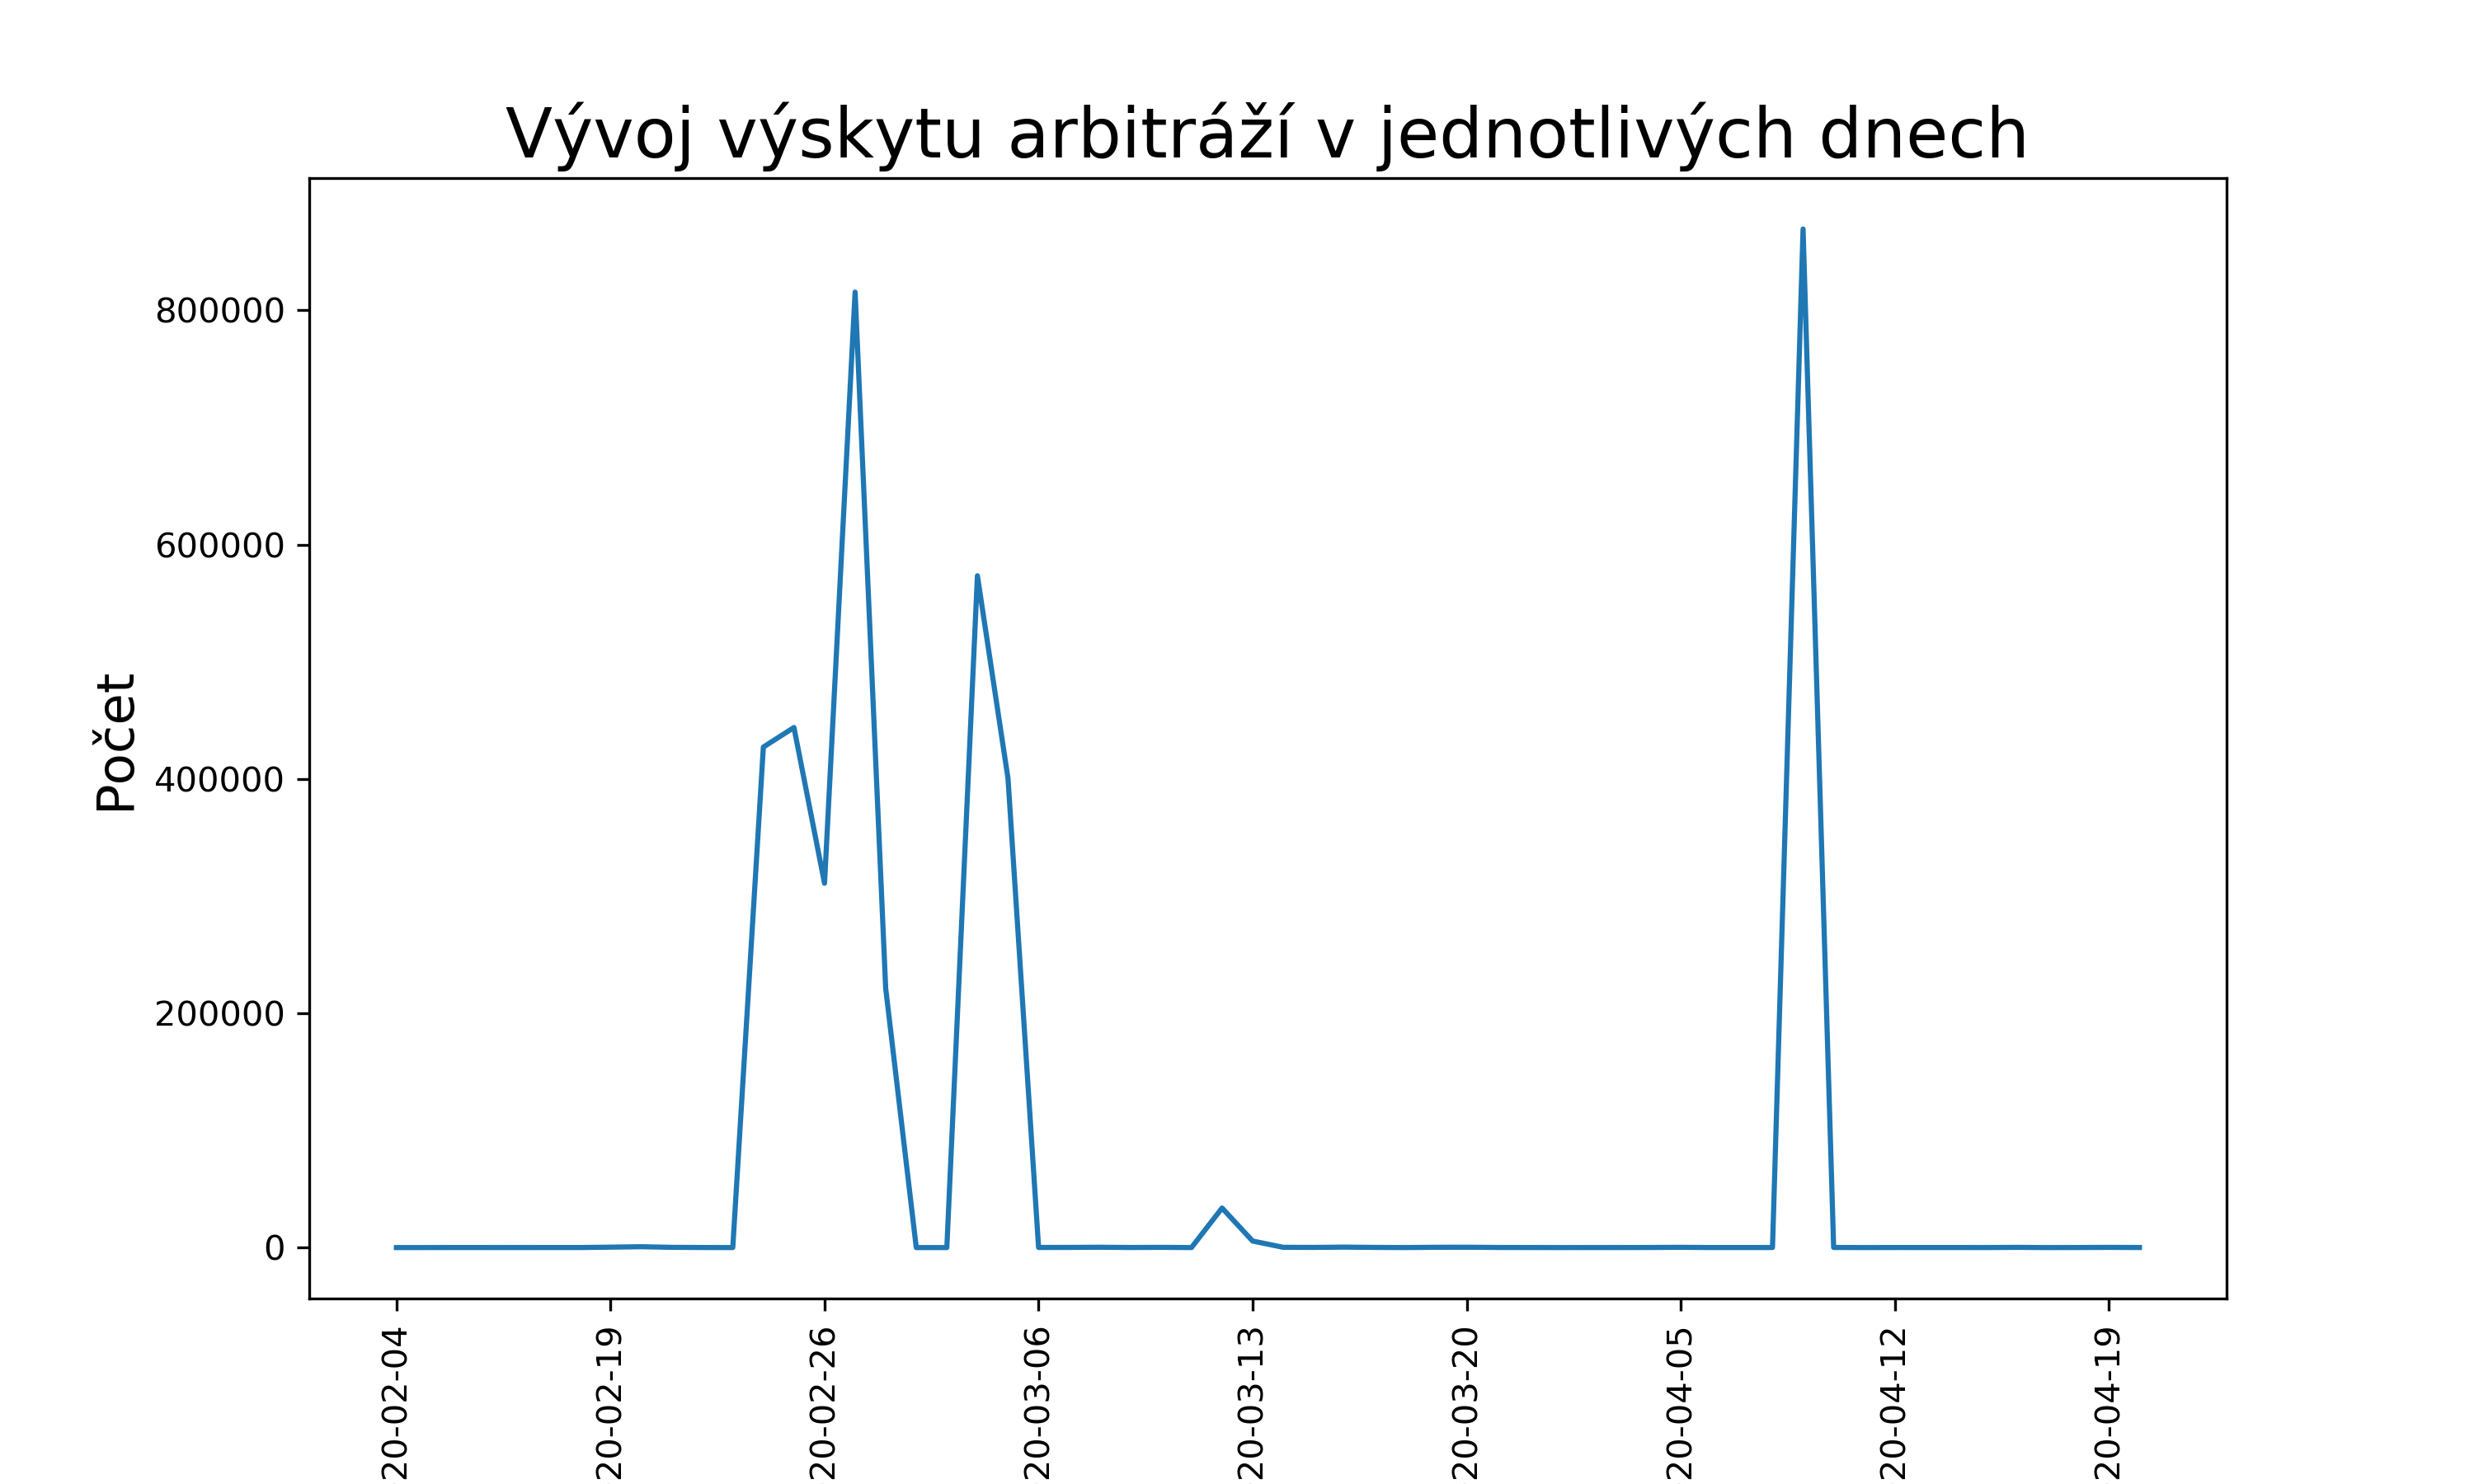
\includegraphics[width=1\textwidth]{images/occurences.png}
	\caption{Rozložení arbitrážních příležitostí v~jednotlivých sledovaných dnech}\label{occurences}
\end{figure}
\subsection{Závislost na~denní hodině}
Z grafu \ref{hours_distribution} je vidět, že nějaké hodiny silně převažují v~počtu výskytu arbitrážních příležitostí. Domnívám se~však, že je to způsobeno stejným jevem, jako v~případě korelace s~dny v~týdnu a~to tím, že se~arbitrážní příležitosti neobjevují rovnoměrně v~čase (viz \ref{occurences}, nýbrž se~vyskytují vždy ve~velkém množství po~krátkou dobu. Tento efekt spojený s~faktem, že nemám dostatečné množství dat poté může způsobovat velké výkyvy v~grafu rozložení v~závislosti na~hodině dne (viz graf \ref{hours_distribution}).

Díky tomuto efektu dále není možné z~mých dat docházet k~jakýmkoliv hlubším závěrům, neboť bych potřeboval, abych měl zaevidovaný vyšší počet výkyvů. Z~toho důvodu nemohu potvrdit ani vyvrátit možnost výskytu korelace mezi výskytem arbitrážních příležitostí a~hodinou ve~dni.

\begin{figure}\centering
	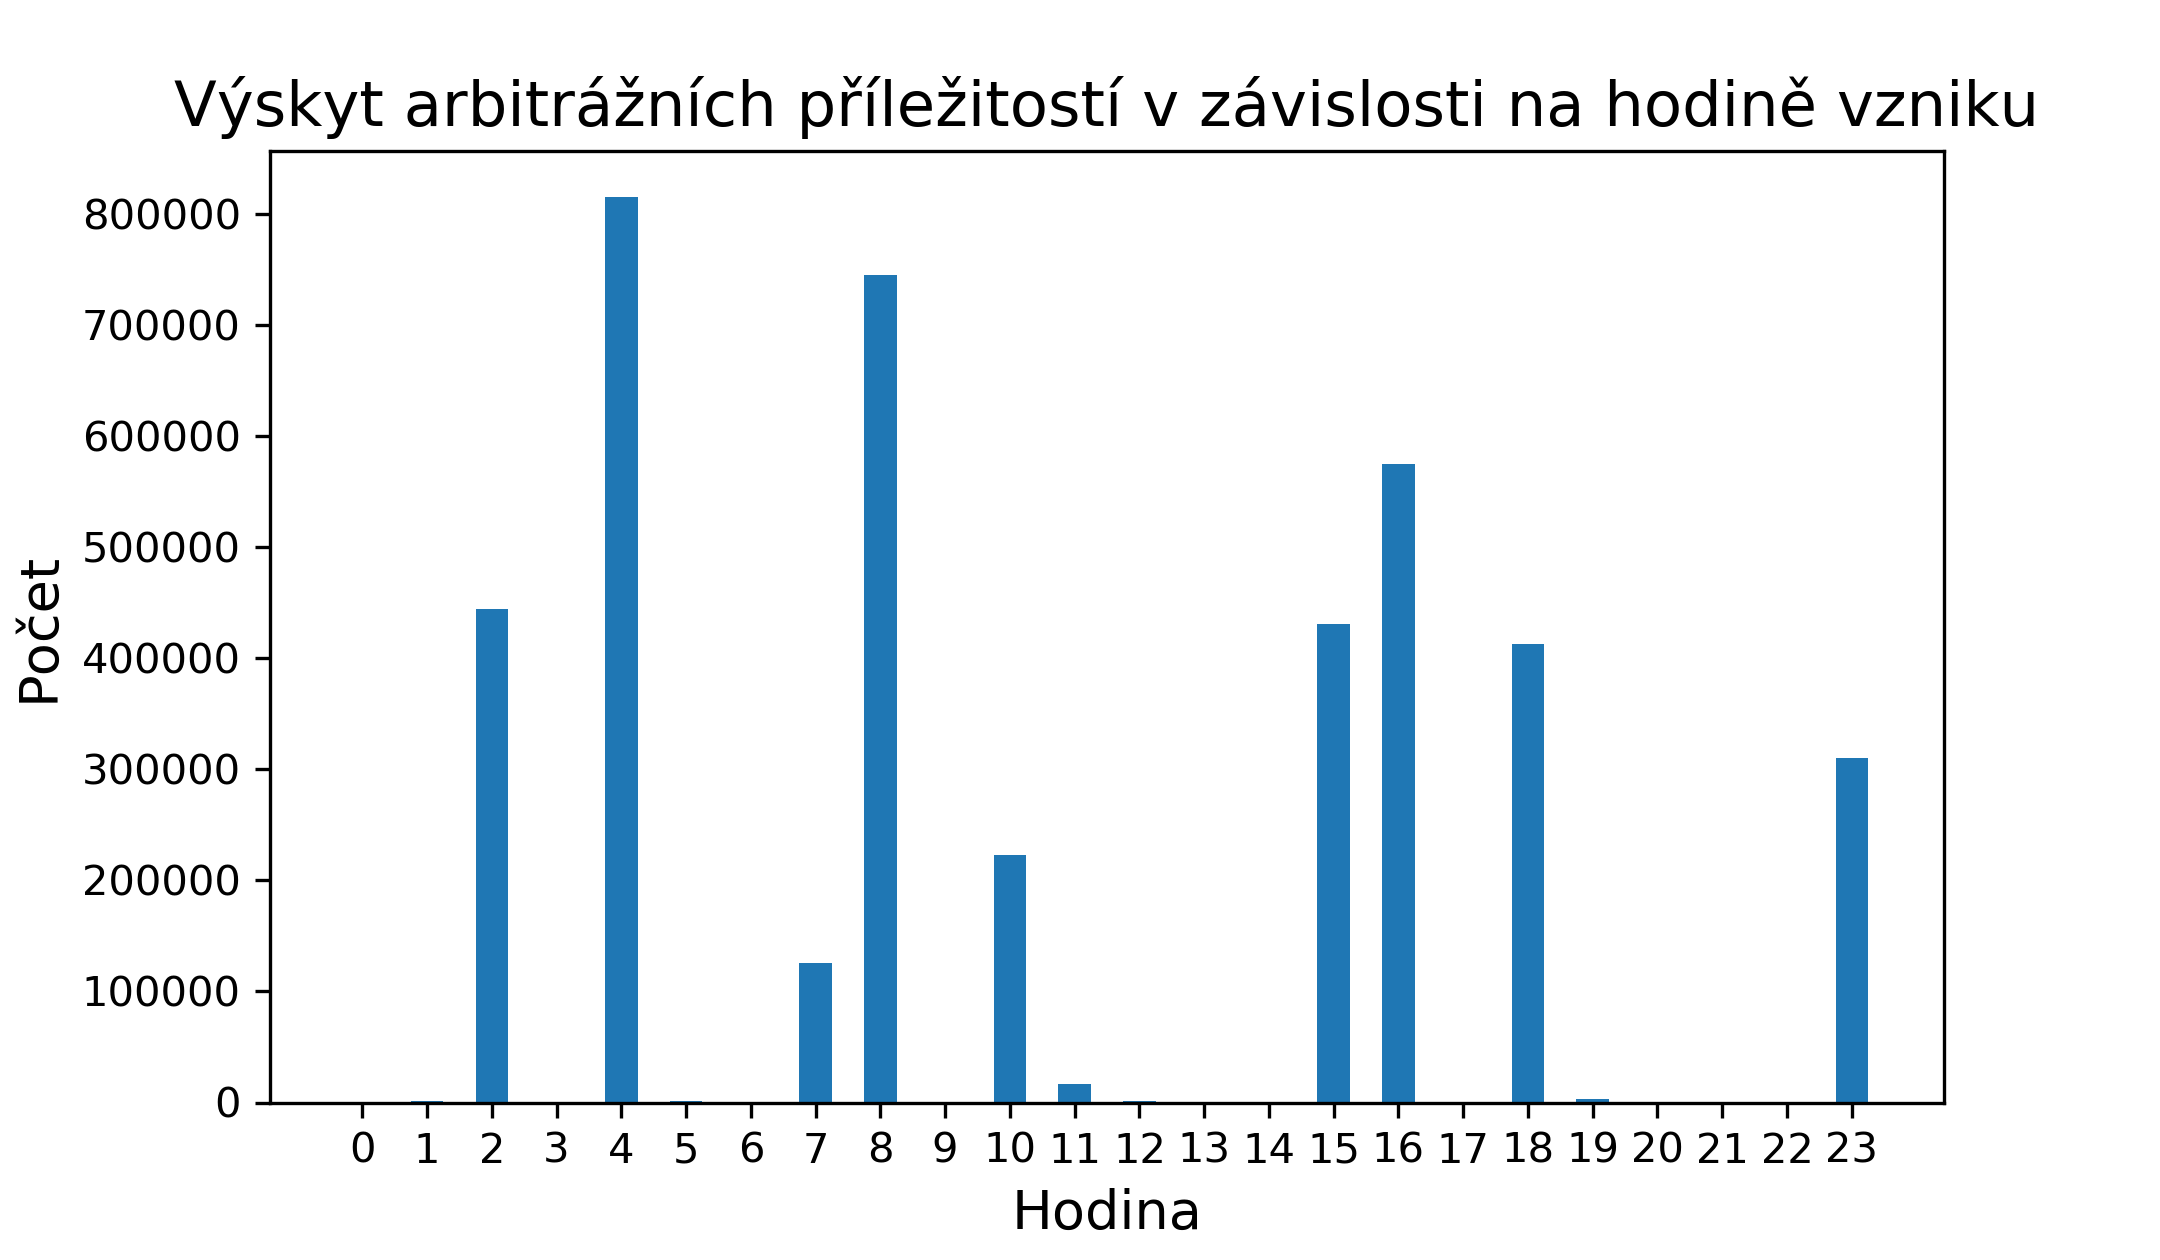
\includegraphics[width=1\textwidth]{images/hours_distribution.png}
	\caption{Rozložení arbitrážních příležitostí v~závislosti na~hodině výskytu }\label{hours_distribution}
\end{figure}
\subsection{Závislost na~počtu provedených transakcí}
Počet transakcí je číslo, které by také mohlo ovlivňovat počet výskytu arbitrážních příležitostí, protože za~předpokladu, že nebudou prováděny žádné transakce, se~nemohou vytvářet ani nové arbitrážní příležitosti.

Pearsonův korelační koeficient diskrétních hodnot s~četností po~jednotlivých dnech těchto dvou veličin vyšel \(\sim-0,085\), z~čehož vyplývá, že tyto dvě veličiny spolu téměř vůbec nekorelují, a~proto není možné mluvit o~jakékoliv závislosti jedné na~druhé (obrázek \ref{occurence_correlation}).

\begin{figure}\centering
	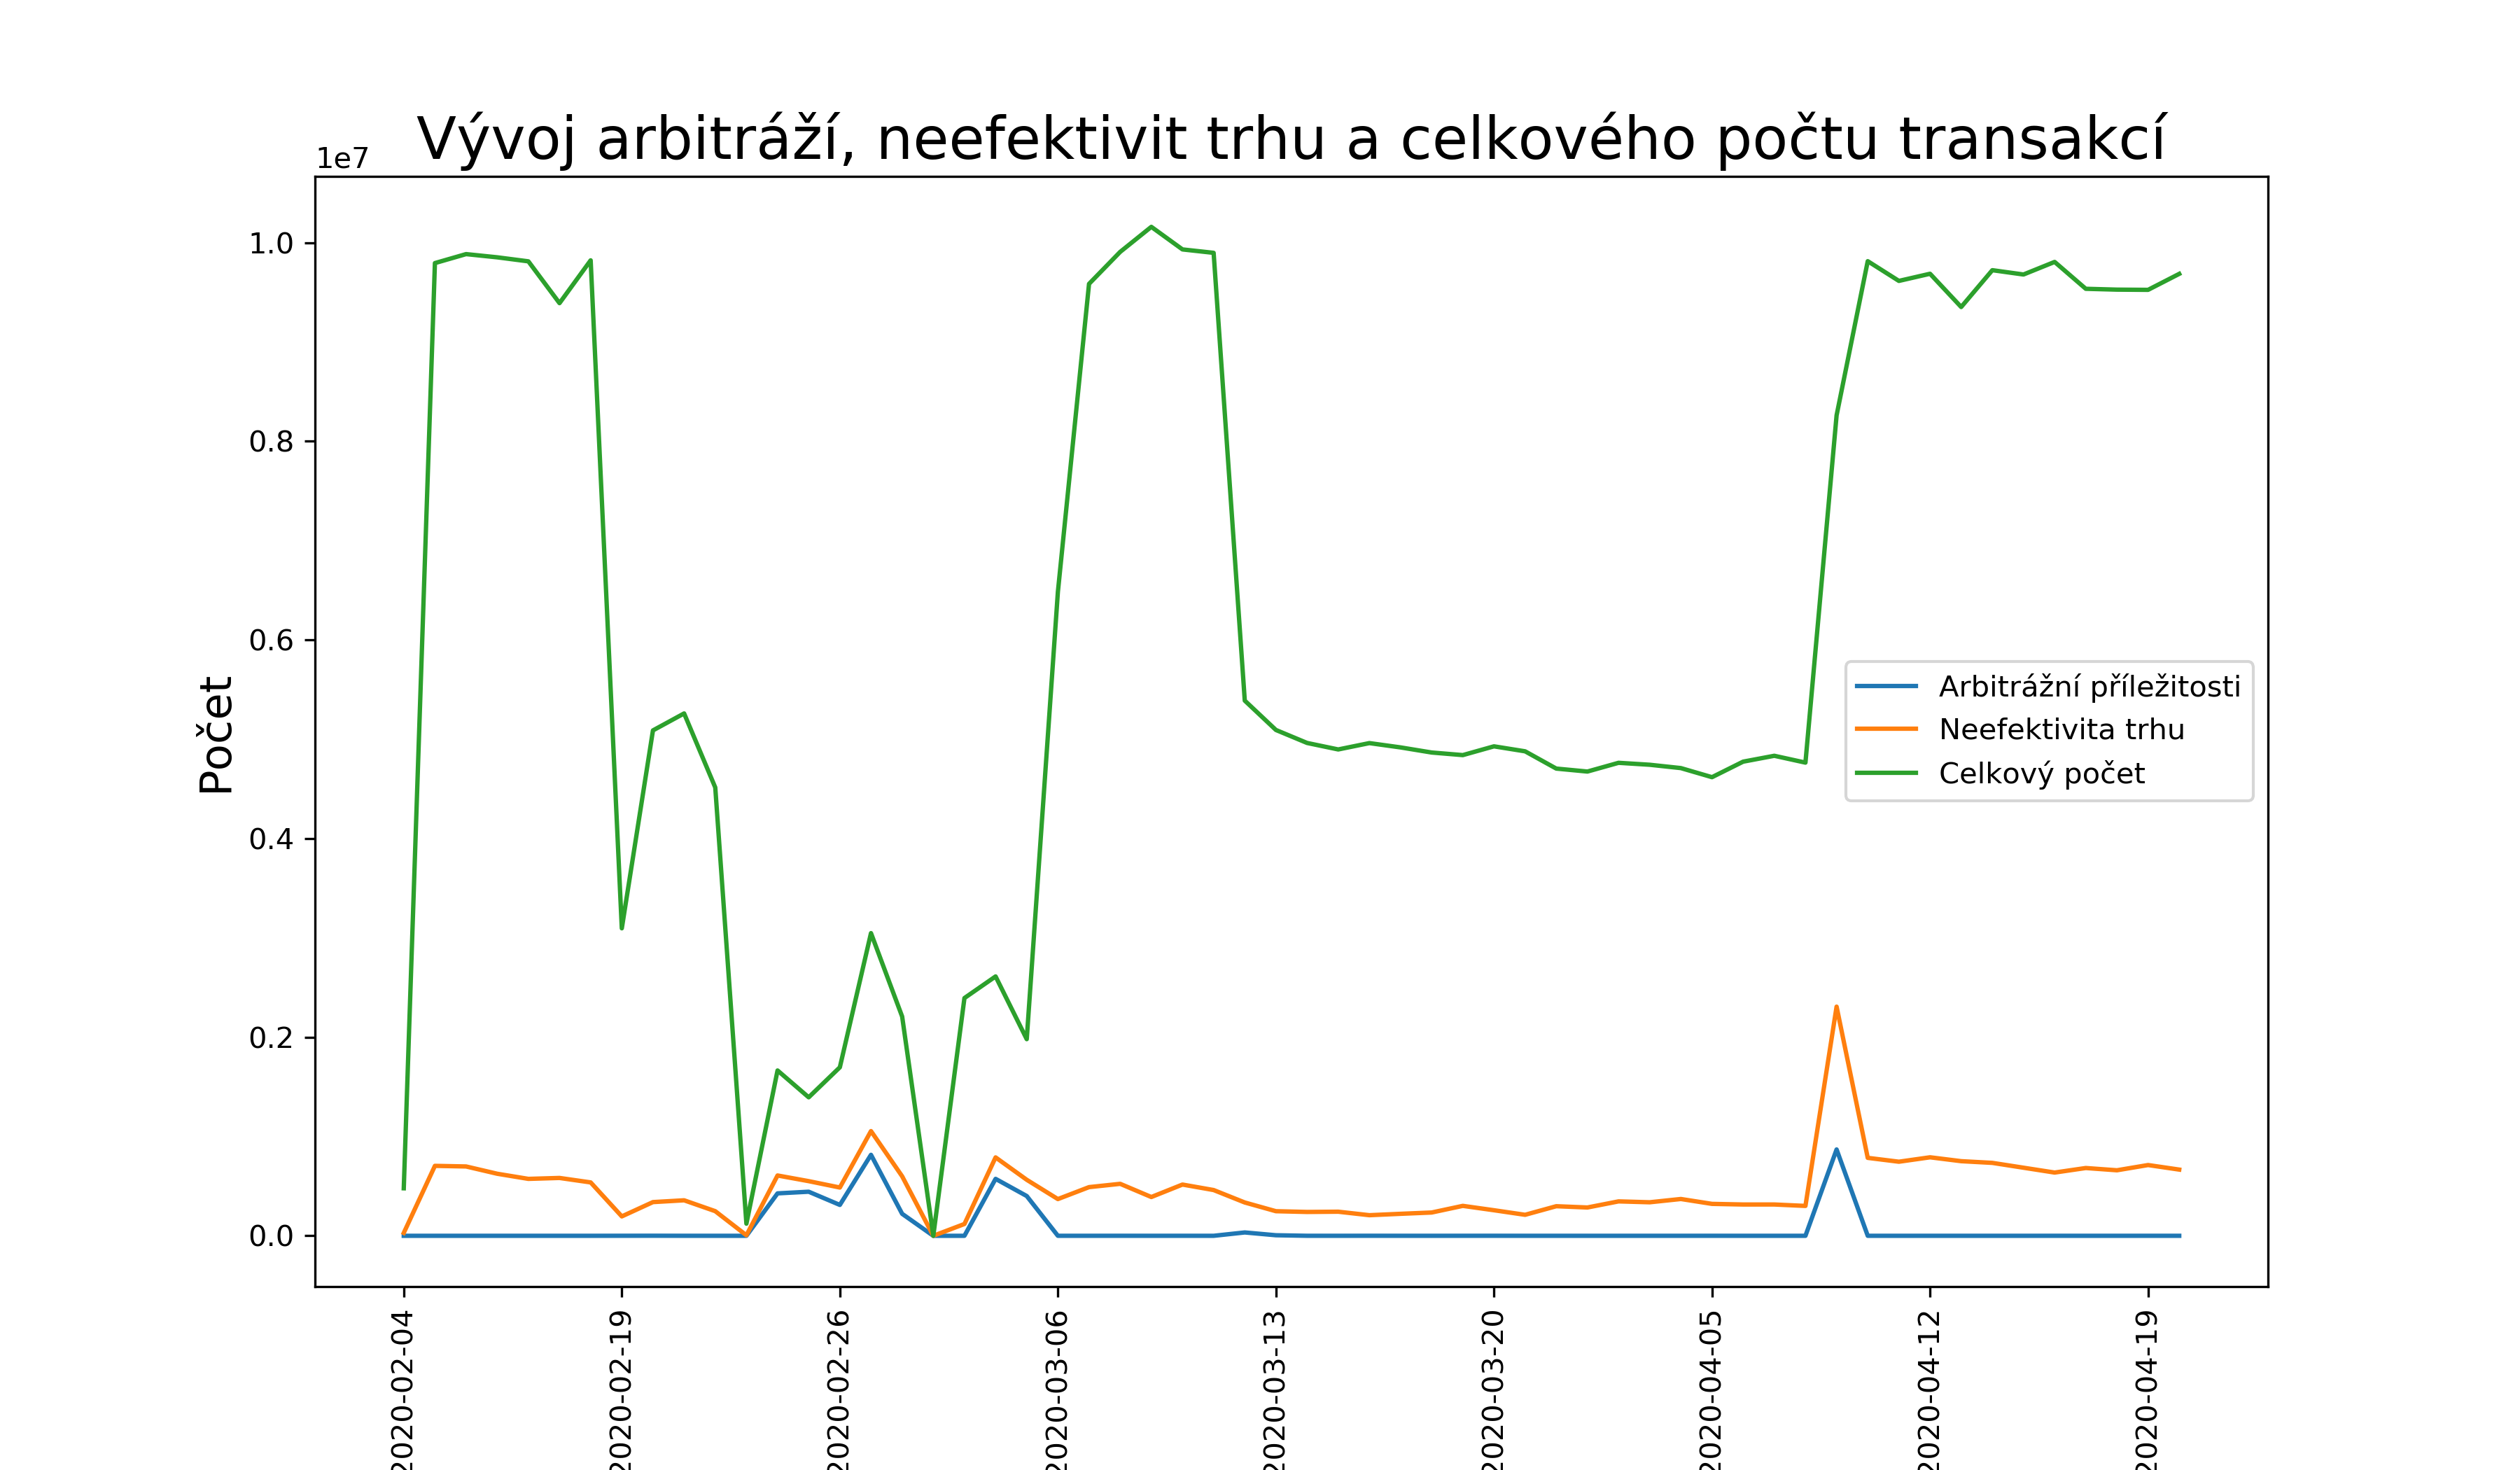
\includegraphics[width=1\textwidth]{images/occurence_correlation.png}
	\caption{Vývoj rozložení výskytu arbitrážních příležitostí, neefektivit trhu a~celkového počtu provedených transakcí po jednotlivých dnech}\label{occurence_correlation}
\end{figure}
\subsection{Závislost na~počtu obecných neefektivit trhu}
Dalším faktorem, na~který jsem se~zaměřil v~souvislosti s~otázku, na~čem by mohl být výskyt arbitrážních příležitostí závislý, je počet neefektivit trhu. Jako neefektivitu trhu označuji takovou situaci, kdy by se~jednalo o~arbitrážní příležitost za~předpokladu, že by nemusely být zahrnuty poplatky. Z~této definice vyplývá, že každá arbitrážní příležitost je také nutně neefektivitou trhu.

Z grafů \ref{ineffictivity_correlation} a~\ref{occurences} je poměrně zřejmé, že výskyt arbitrážních příležitostí a~neefektivit trhu spolu moc nekorelují. Výpočet Pearsonova korelačního koeficientu diskrétních hodnot braných po~jednotlivých dnech to potvrzuje výsledkem \(\sim-0,090\). Z~korelačního koeficientu tedy plyne, že tyto dvě hodnoty spolu téměř nekorelují.

\begin{figure}\centering
	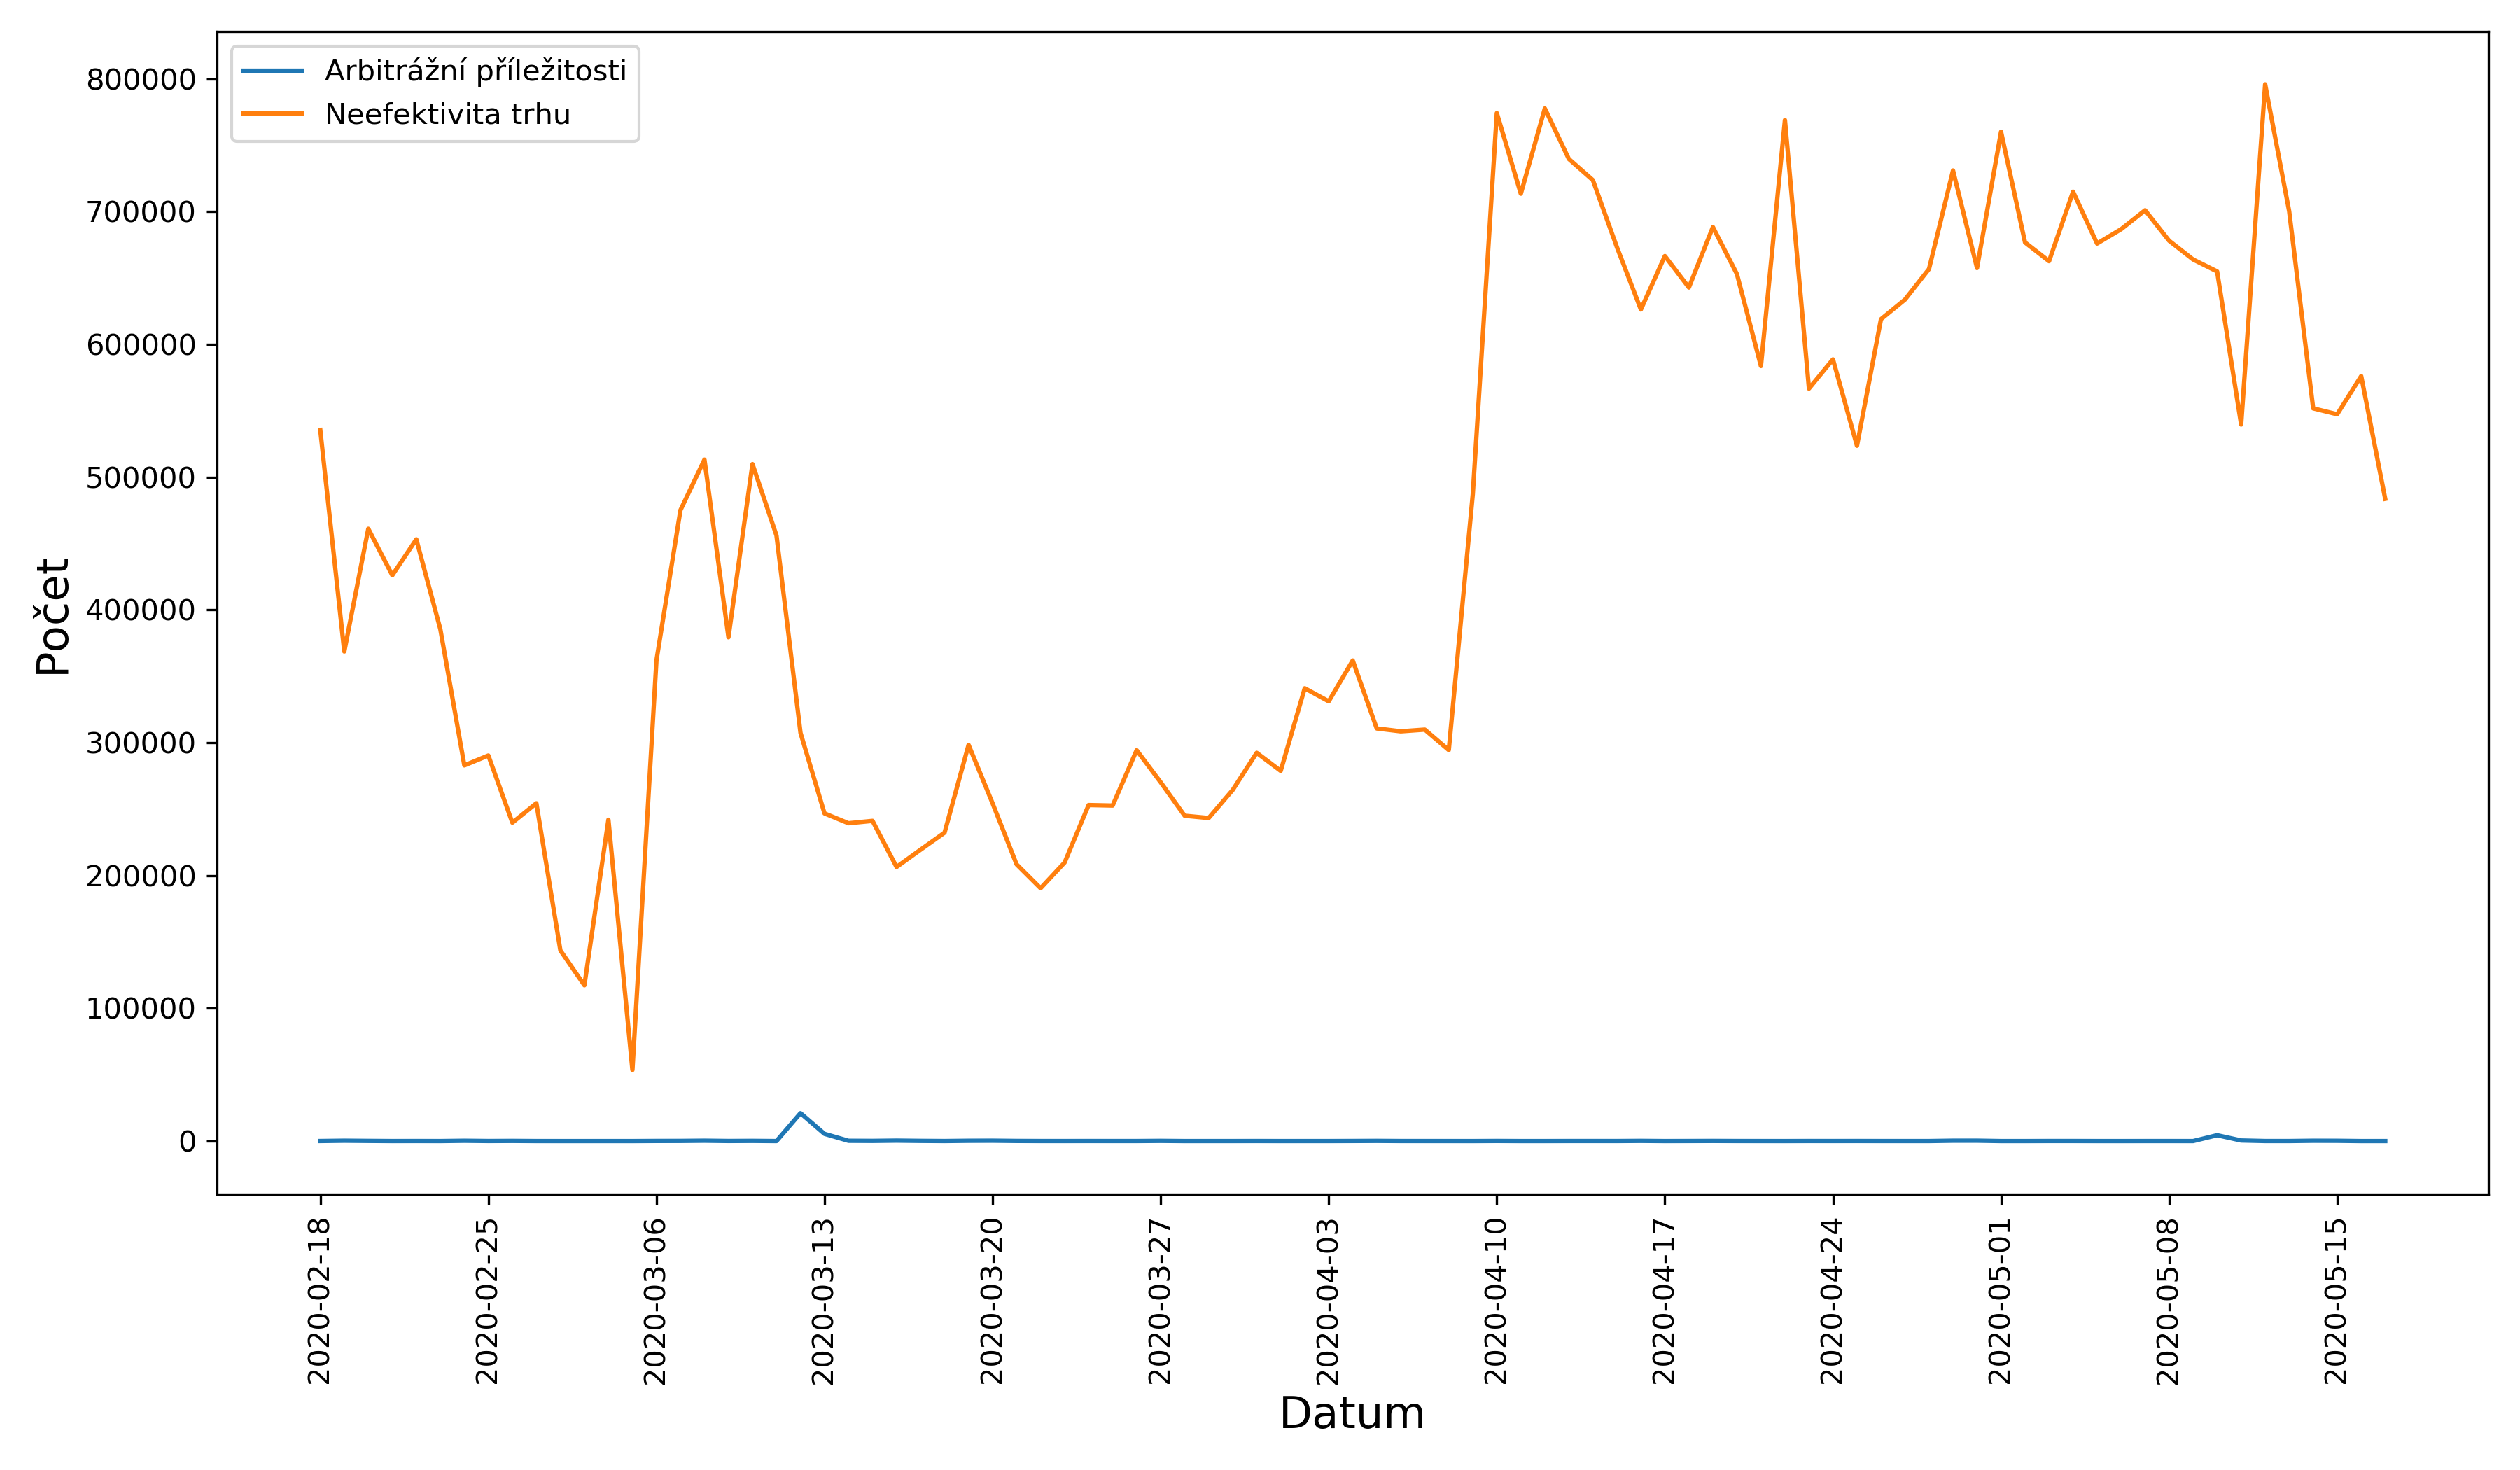
\includegraphics[width=1\textwidth]{images/ineffictivity_correlation.png}
	\caption{Vývoj rozložení výskytu arbitrážních příležitostí a~neefektivit trhu po jednotlivých dnech}
	\label{ineffictivity_correlation}
\end{figure}

\section{Konkrétní hodnoty nejzajímavějších trojúhelníků}
V této sekci se~podrobněji věnuji nejzajímavějším trojúhelníkům, které jsem vyselektoval na~základě téměř tří měsíců dat. 

\subsection{Selekce}
Trojúhelníky jsem vybíral převážně na~základě hodnot z~předchozí sekce \linebreak (konkrétně z~tabulek \ref{table_averages} a~\ref{table_gains}). Z~toho důvodu, že se~většina pozorovaných hodnot mezi jednotlivými měnami moc neliší, bral jsem v~potaz převážně faktor průměrného denního potenciálního zisku (ne všechny trojúhelníky mají data ze všech dní, proto byl zvolen průměr).

V tabulce \ref{table_combined_best} jsou ponechány pouze záznamy, u~kterých je možné v~průměru každý den vydělat více než 10 amerických dolarů. V~této sekci se~však nevěnuji všem, ale pouze pěti nejlukrativnějším trojúhelníkům a jednomu zajímavému kvůli jeho odlišným vlastnostem (USDT/BTC/BCH). Nevěnuji se všem trojúhelníkům splňující spodní podmínku výdělečnosti, poněvadž mají velmi podobné vlastnosti a tabulky k ostatním jsou uvedeny v příloze.

Je zajímavé si povšimnout, že ve~všech nejzajímavějších trojúhelnících figuruje USD Tether, zástupce stabilní měny odpovídající americkému dolaru.


\begin{table}\centering
\caption{Průměrné denní hodnoty arbitrážních příležitostí na nejlepších trojúhelnících}
\label{table_combined_best}
\begin{tabular}{|| l | r | r ||}\hline Trojúhelník & Průměrný denní počet & Denní neefektivita (USD)\\
 \hline
 \hline USDT/EOS/BNB & 18,229885 & 178,495958\\ 
 \hline USDT/BTC/EOS & 13,367816 & 119,419172\\ 
 \hline USDT/BNB/XMR & 28,941176 & 110,616732\\ 
 \hline USDT/BTC/XRP & 14,402299 & 105,499992\\ 
 \hline USDT/BTC/TRX & 6,321839 & 105,073403\\ 
 \hline USDT/XRP/BNB & 12,862069 & 104,913628\\ 
 \hline USDT/BTC/LTC & 12,908046 & 99,765406\\ 
 \hline USDT/LTC/BNB & 17,701149 & 87,437498\\ 
 \hline USDT/BCH/BNB & 19,376471 & 85,079456\\ 
 \hline USDT/BTC/XMR & 20,413793 & 53,204728\\ 
 \hline USDT/XRP/TRX & 30,952941 & 24,070239\\ 
 \hline USDT/BTC/BNB & 7,016667 & 20,742392\\ 
 \hline USDT/BTC/ETH & 3,683333 & 19,901603\\ 
 \hline USDT/BTC/BCH & 4,633333 & 17,886043\\ 
 \hline
\end{tabular}
\end{table}

\subsection{Bližší statistiky}
V této sekci vypisuji konkrétní statistiky k~vybraným zajímavým trojúhelníkům. Statistiky ve~formě tabulek a~grafů ve~stejném formátu ke~všem ostatním trojúhelníkům jsou k~dispozici v~příloze.

\subsubsection{USDT/EOS/BNB}
Trojúhelník USDT/EOS/BNB je z~pohledu potenciálního zisku nejlepší, je však nutné podotknout, že pro zobchodování nějakých příležitostí by bylo nutné provést velmi velké transakce. Například na~nejvýhodnější příležitosti bylo možné vydělat 460,43~EOS (1123,44~USD) viz tabulka \ref{USDTEOSBNB_stats}. Touto nejvýdělečnější transakcí se tak dalo vydělat více než 6,6~\% celkového potenciálního zisku za téměř tři měsíce. Pro uskutečnění takto velké transakce je však nutné zobchodovat obrovské množství peněz (14~745~EOS tedy asi 35~977~USD), které si dovoluji tvrdit, že většina běžných obchodníků na~kontě připravené nemá.

Tento trojúhelník má i nadprůměrně dlouhou dobu trvání výskytu pozitivní arbitrážní příležitosti 0,41~s (průměr činí 0,35~s a medián 0,25~s). Zajímavé je, že k získání poloviny celkového pozorovaného potenciálního zisku stačilo zobchodovat pouze 12 arbitrážních příležitostí s nejvyšším absolutním ziskem. Zbylých 1449 arbitrážních příležitostí tvořilo druhou polovinu celkového potenciálního zisku.

Průměrně se~každý den vyskytne na~tomto trojúhelníku přes 18 arbitrážních příležitostí, toto číslo je však velmi ovlivněno lokálními výkyvy (viz graf \ref{occurences_arbitrage_USDTEOSBN}), a~proto denní medián výskytu činí pouhý 1 výskyt za den.

\begin{table}\centering
\caption{Základní statistiky trojúhelníku USDT/EOS/BNB}
\label{USDTEOSBNB_stats}
\begin{tabular}{|| l | r ||}
\hline Název & Hodnota \\ 
\hline\hline Název & USDT/EOS/BNB \\ 
\hline Počet dní & 87 \\ 
\hline Průměrný denní počet arbitráží & 18,229885057471265 \\ 
\hline Medián denního počtu arbitráží & 1,0 \\ 
\hline Průměrný procentuální zisk & 1,0006779030220183 \\ 
\hline Nejvyšší procentuální zisk & 1,099279716 \\ 
\hline Celkový potenciální zisk & 6364,405072 EOS \\ 
\hline Celkový potenciální zisk (USD) & 15529,148376552923 \\ 
\hline Průměrný denní potenciální zisk & 73,154081 EOS \\ 
\hline Průměrný denní potenciální zisk (USD) & 178,49595835118302 \\ 
\hline Nejvyšší potenciální zisk & 460,426732 EOS \\ 
\hline Nejvyšší potenciální zisk (USD) & 1123,441226324 \\ 
\hline Průměrná doba trvání & 0,4055661658894621 \\ 
\hline Celkový počet příležitostí & 2693 \\ 
\hline Počet příležitostí k zisku poloviny celkového zisku & 12 \\ 
\hline
\end{tabular}
\end{table}

\begin{figure}\centering
	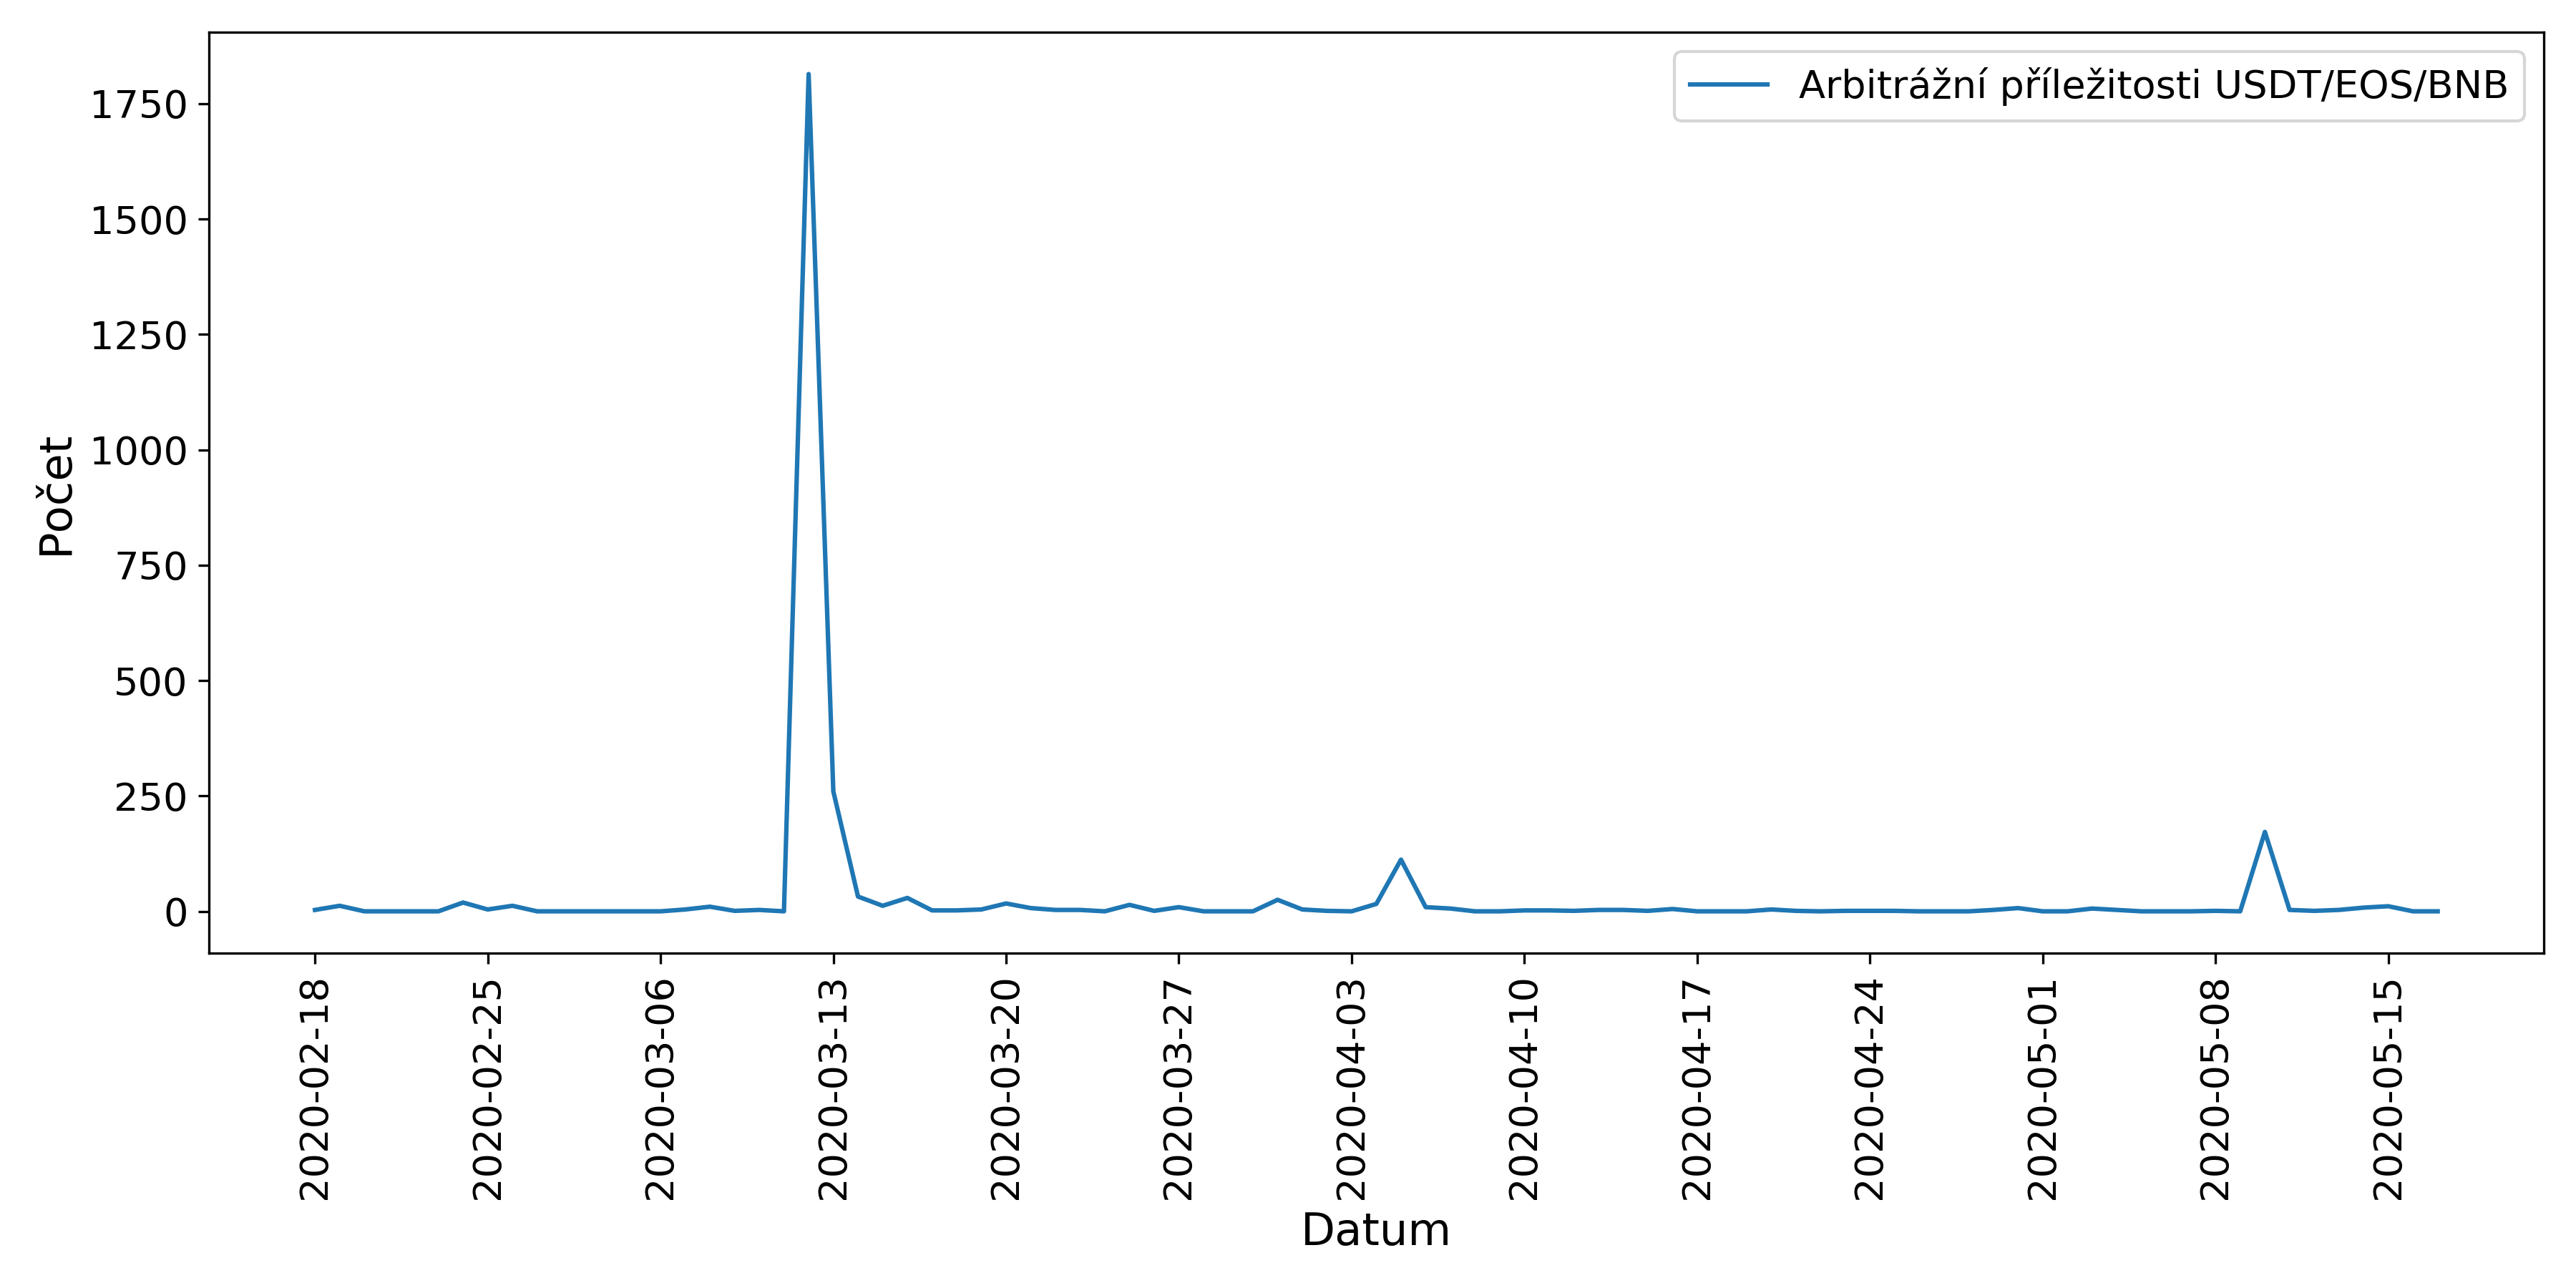
\includegraphics[width=1\textwidth]{images/best_triangles/occurences_arbitrage_USDTEOSBNB.png}
	\caption{Vývoj arbitrážních příležitostí na~trojúhelníku USDT/EOS/BNB }\label{occurences_arbitrage_USDTEOSBN}
\end{figure}


\subsubsection{Trojúhelník USDT/BTC/EOS}
Trojúhelník USDT/BTC/EOS je z~pohledu potenciálního zisku druhým nevýdělečnějším. Oproti trojúhelníku USDT/EOS/BNB je vyváženější z pohledu výkyvů ve~velikosti příležitostí, nejvýdělečnější transakce zahrnuje pouze 2,5~\% celkového potenciálního zisku (viz tabulka \ref{USDTBTCEOS_stats}). Tento trojúhelník má podprůměrně dlouhou dobu trvání výskytu pozitivní arbitrážní příležitosti 0,33~s (průměr činí 0,35~s a medián 0,25~s). 

Průměrně se~v~každý den vyskytne na~tomto trojúhelníku přes 13 arbitrážních příležitostí, toto číslo je však velmi ovlivněno lokálními výkyvy (viz graf \ref{occurences_arbitrage_USDTBTCEOS}), a~proto denní medián nečiní žádný výskyt.

\begin{table}\centering
\caption{Základní statistiky trojúhelníku USDT/BTC/EOS}
\label{USDTBTCEOS_stats}
\begin{tabular}{|| l | r ||}
\hline Název & Hodnota \\ 
\hline\hline Název & USDT/BTC/EOS \\ 
\hline Počet dní & 87 \\ 
\hline Průměrný denní počet arbitráží & 13,367816091954023 \\ 
\hline Medián denního počtu arbitráží & 0,0 \\ 
\hline Průměrný procentuální zisk & 1,0006232934708796 \\ 
\hline Nejvyšší procentuální zisk & 1,073843096 \\ 
\hline Celkový potenciální zisk & 4257,978680 EOS \\ 
\hline Celkový potenciální zisk (USD) & 10389,467979647266 \\ 
\hline Průměrný denní potenciální zisk & 48,942284 EOS \\ 
\hline Průměrný denní potenciální zisk (USD) & 119,41917217985363 \\ 
\hline Nejvyšší potenciální zisk & 95,706220 EOS \\ 
\hline Nejvyšší potenciální zisk (USD) & 233,5231760436 \\ 
\hline Průměrná doba trvání & 0,3288854242482326 \\ 
\hline Celkový počet příležitostí & 1461 \\ 
\hline Počet příležitostí k zisku poloviny celkového zisku & 47 \\ 
\hline
\end{tabular}
\end{table}

\begin{figure}\centering
	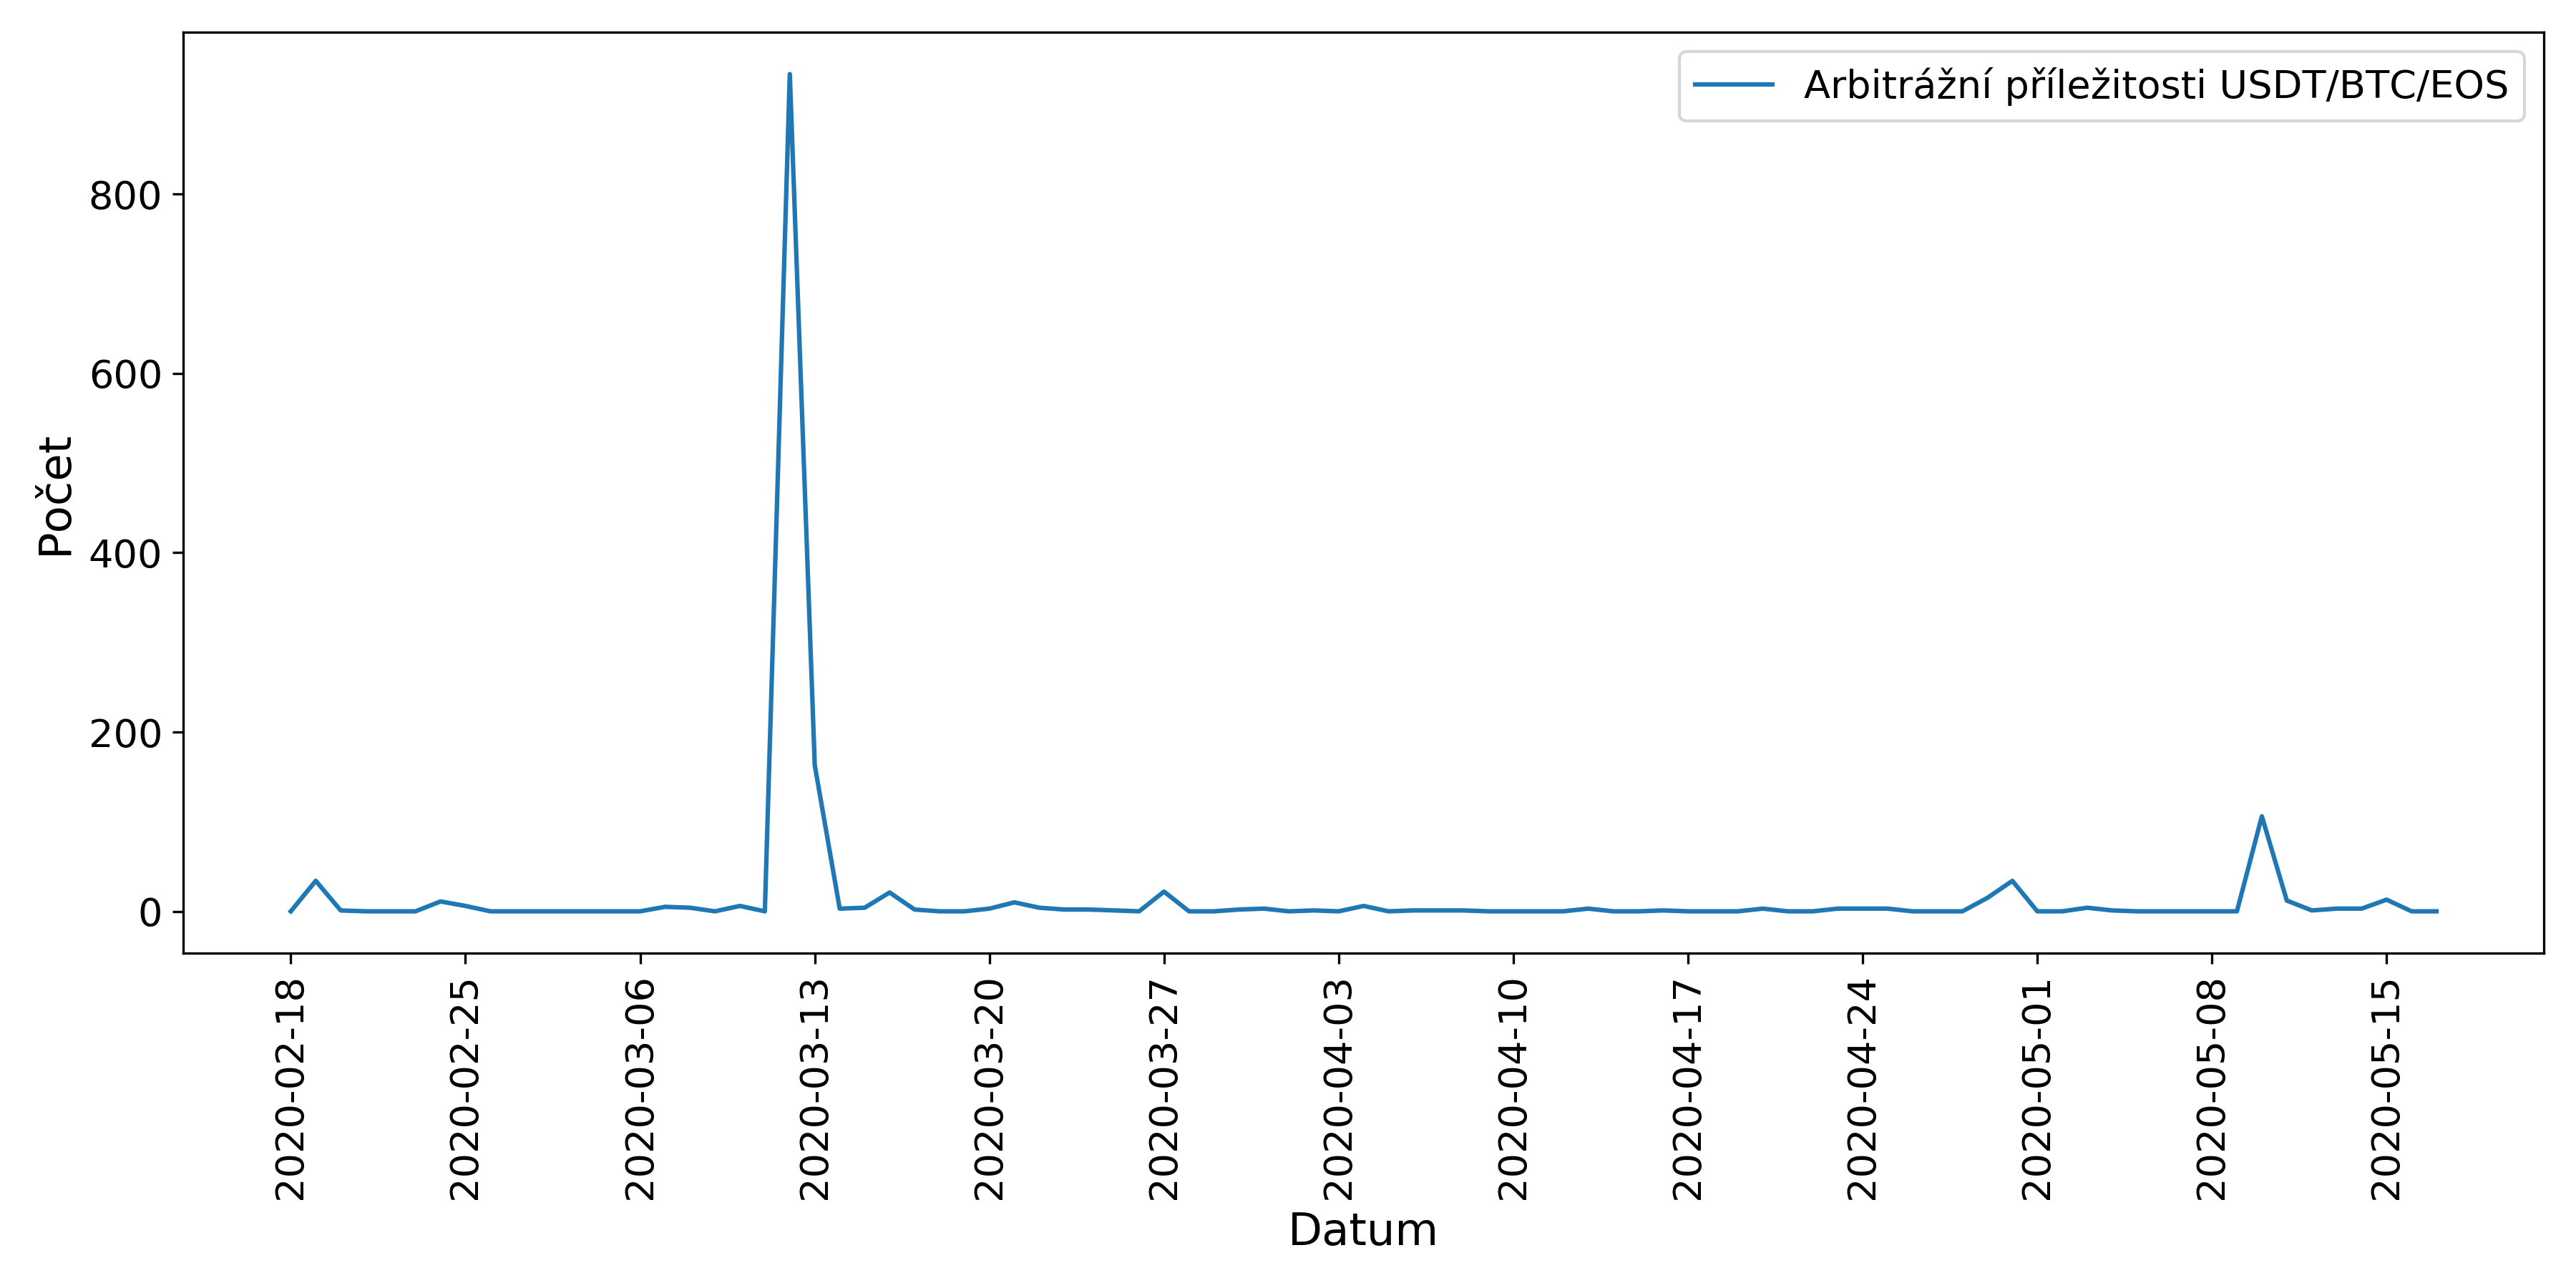
\includegraphics[width=1\textwidth]{images/best_triangles/occurences_arbitrage_USDTBTCEOS.png}
	\caption{Vývoj arbitrážních příležitostí na~trojúhelníku USDT/BTC/EOS }\label{occurences_arbitrage_USDTBTCEOS}
\end{figure}

\subsection{Trojúhelník USDT/BNB/XMR}
Trojúhelník USDT/BNB/XMR je třetím nejvýdělečnějším trojúhelníkem \linebreak a~svými vlastnostmi se velmi podobá předchozím dvěma trojúhelníkům. Průměrný denní počet výskytů (téměř 29 za den) také velice převyšuje denní medián výskytů, pouze 1 (viz tabulka \ref{USDTBNBXMR_stats} a graf \ref{occurences_arbitrage_USDTBNBXMR}). Trojúhelník má \linebreak podprůměrnou dobu výskytu pozitivní arbitrážní příležitosti, pouze 0,34 (průměr činí 0,35~s a medián 0,25~s).

Zajímavou hodnotou na tomto trojúhelníku je, že z celkových 4349 pozitivních arbitrážní příležitostí pokrylo polovinu celkového potenciálního zisku pouze 16 arbitráží (0,37~\% arbitrážních příležitostí pokrylo více než 50~\% celkového potenciálního zisku).

\begin{table}\centering
\caption{Základní statistiky trojúhelníku USDT/BNB/XMR}
\label{USDTBNBXMR_stats}
\begin{tabular}{|| l | r ||}
\hline Název & Hodnota \\ 
\hline\hline Název & USDT/BNB/XMR \\ 
\hline Počet dní & 85 \\ 
\hline Průměrný denní počet arbitráží & 28,941176470588236 \\ 
\hline Medián denního počtu arbitráží & 1,0 \\ 
\hline Průměrný procentuální zisk & 1,000667765324073 \\ 
\hline Nejvyšší procentuální zisk & 1,12956548 \\ 
\hline Celkový potenciální zisk & 176,174297 XMR \\ 
\hline Celkový potenciální zisk (USD) & 9402,422255187845 \\ 
\hline Průměrný denní potenciální zisk & 2,072639 XMR \\ 
\hline Průměrný denní potenciální zisk (USD) & 110,61673241397463 \\ 
\hline Nejvyšší potenciální zisk & 9,045483 XMR \\ 
\hline Nejvyšší potenciální zisk (USD) & 482,75741420738996 \\ 
\hline Průměrná doba trvání & 0,33822535252042407 \\ 
\hline Celkový počet příležitostí & 4349 \\ 
\hline Počet příležitostí k zisku poloviny celkového zisku & 16 \\ 
\hline
\end{tabular}
\end{table}

\begin{figure}\centering
	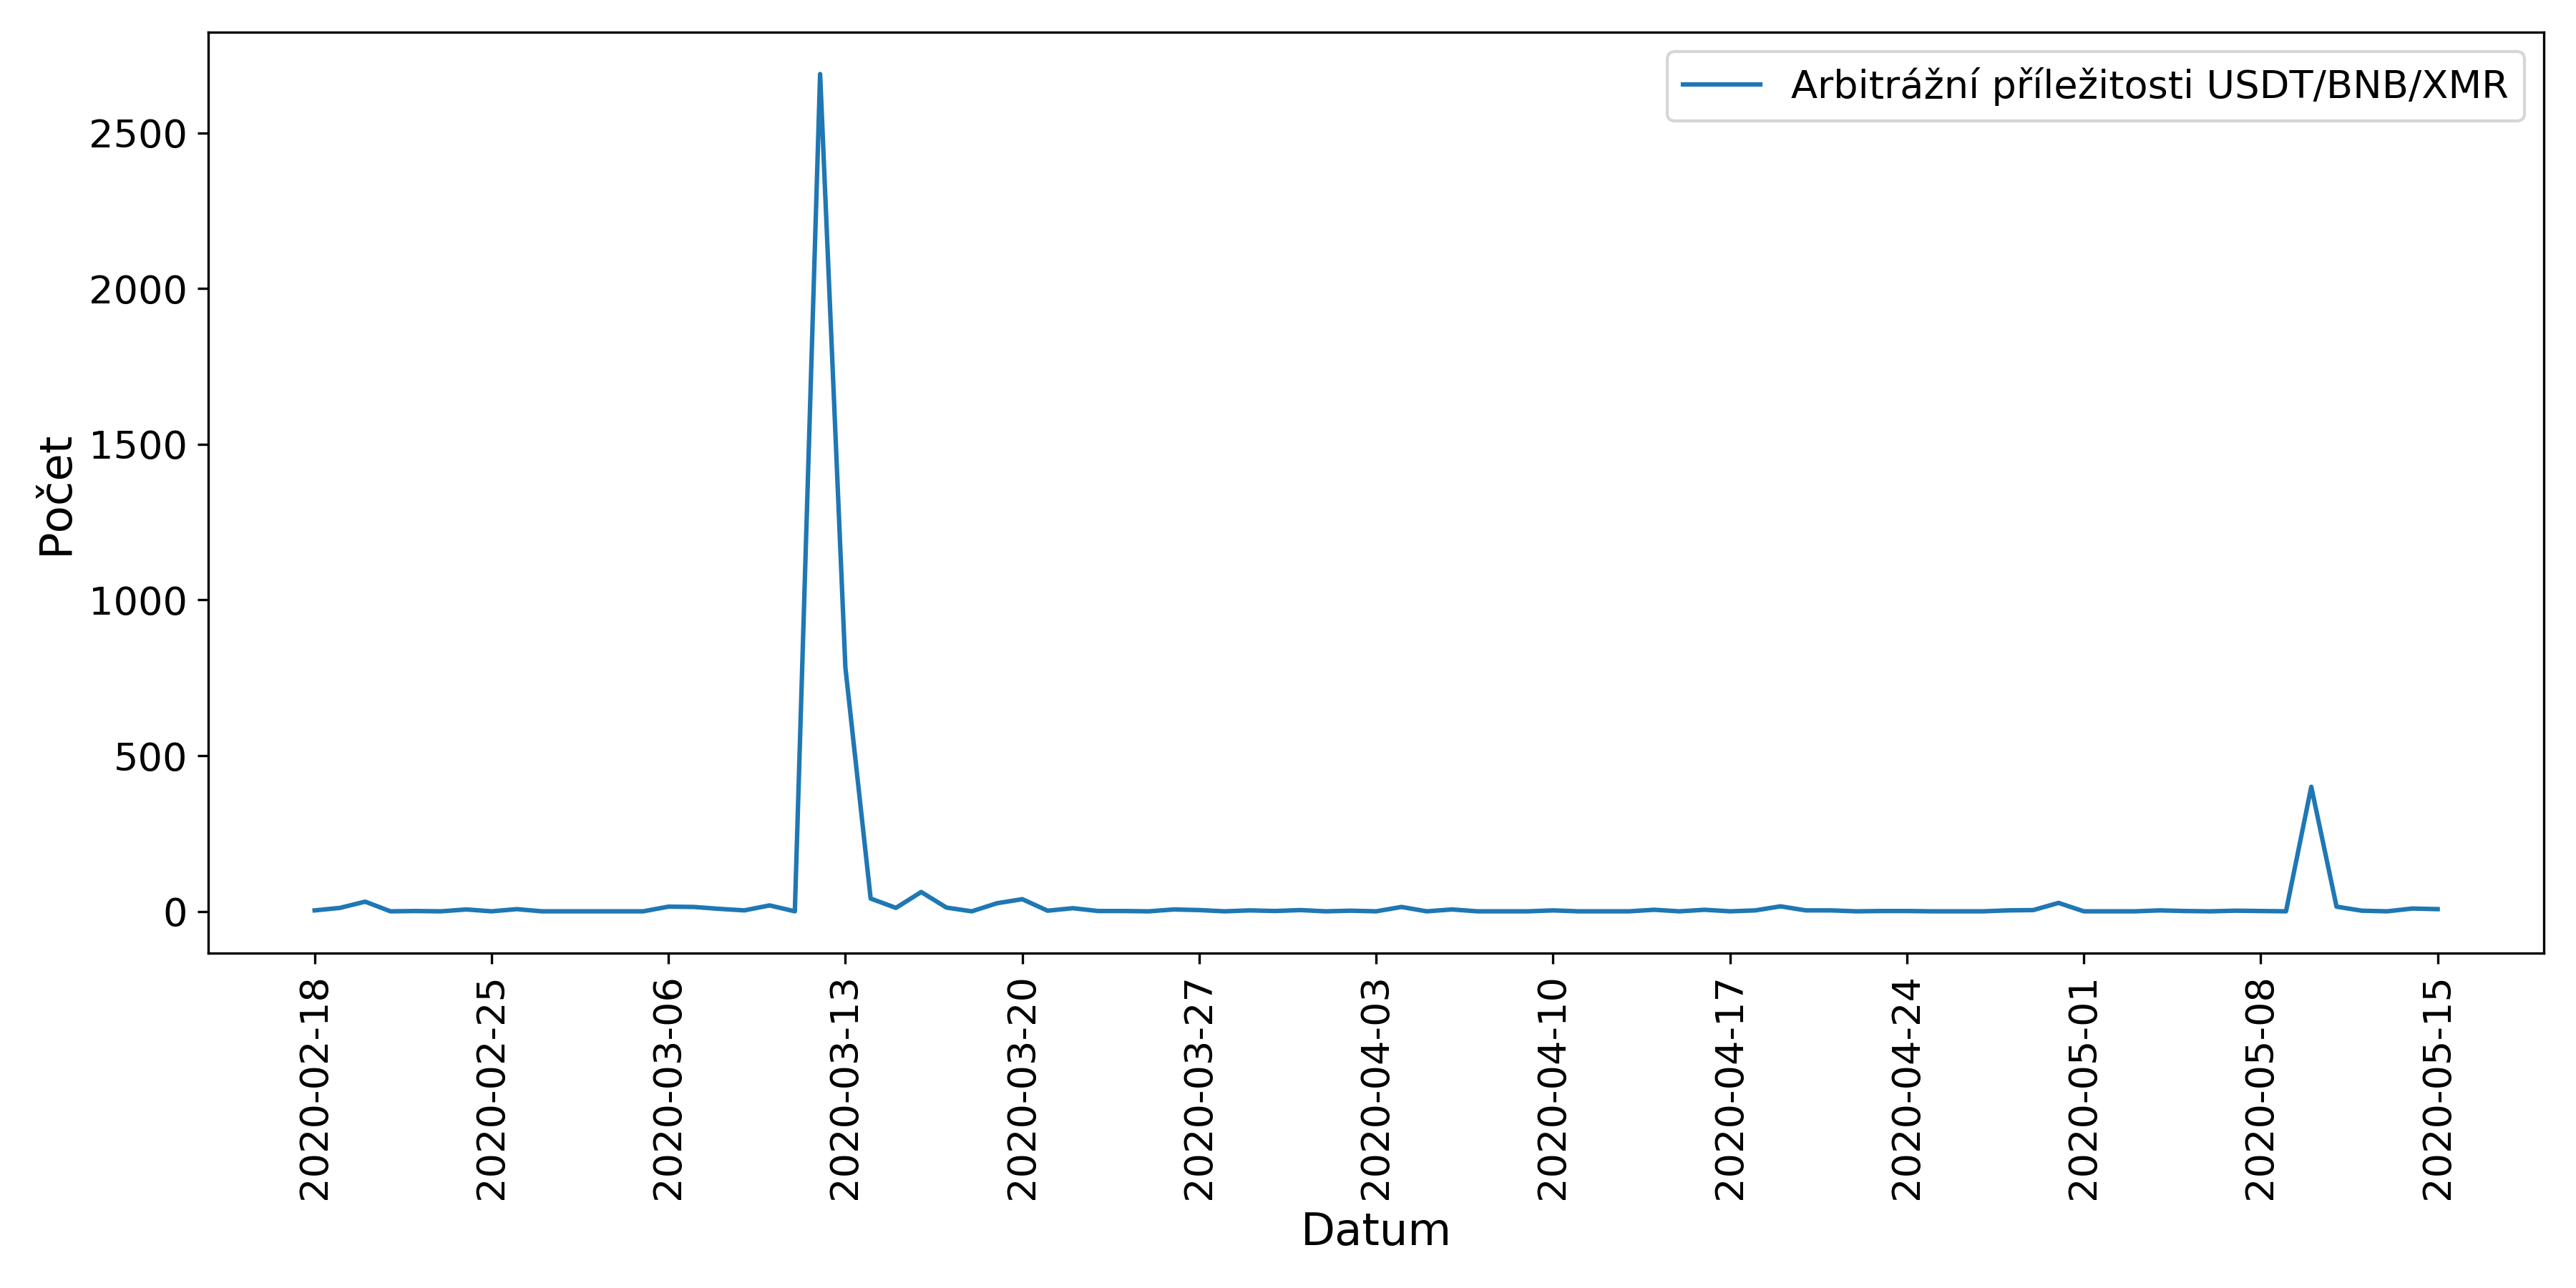
\includegraphics[width=1\textwidth]{images/best_triangles/occurences_arbitrage_USDTBNBXMR.png}
	\caption{Vývoj arbitrážních příležitostí na~trojúhelníku USDT/BNB/XMR }\label{occurences_arbitrage_USDTBNBXMR}
\end{figure}

\subsubsection{Trojúhelník USDT/BTC/XRP}
Trojúhelník USDT/BTC/XRP je z~pohledu výše celkového potenciálního zisku čtvrtý nejlepší. Trpí však podobnými problémy jako předchozí trojúhelníky. Denně se průměrně objevuje přes 14 arbitrážních příležitostí, avšak medián výskytu je nulový, tedy během většiny dní se na trojúhelníku nic zajímavého neděje. 

Vysoký rozdíl mezi průměrem a mediánem počtu výskytů je taktéž způsoben velkým výkyvem z~12.~a~13.~března 2020 (viz graf \ref{occurences_arbitrage_USDTBTCXRP} a~tabulka \ref{USDTBTCXRP_stats}). Trojúhelník USDT/BTC/XRP má nadprůměrně dlouhé trvání pozitivních arbitrážních příležitostí a to 0,38~s (průměr činí 0,35~s a medián 0,25~s).

\begin{table}\centering
\caption{Základní statistiky trojúhelníku USDT/BTC/XRP}
\label{USDTBTCXRP_stats}
\begin{tabular}{|| l | r ||}
\hline Název & Hodnota \\ 
\hline\hline Název & USDT/BTC/XRP \\ 
\hline Počet dní & 87 \\ 
\hline Průměrný denní počet arbitráží & 14,402298850574713 \\ 
\hline Medián denního počtu arbitráží & 0,0 \\ 
\hline Průměrný procentuální zisk & 1,0005281442944596 \\ 
\hline Nejvyšší procentuální zisk & 1,057942892 \\ 
\hline Celkový potenciální zisk & 49356,057687 XRP \\ 
\hline Celkový potenciální zisk (USD) & 9178,49926772779 \\ 
\hline Průměrný denní potenciální zisk & 567,311008 XRP \\ 
\hline Průměrný denní potenciální zisk (USD) & 105,49999158307804 \\ 
\hline Nejvyšší potenciální zisk & 1226,628320 XRP \\ 
\hline Nejvyšší potenciální zisk (USD) & 228,1099355288 \\ 
\hline Průměrná doba trvání & 0,38476166983032234 \\ 
\hline Celkový počet příležitostí & 1572 \\ 
\hline Počet příležitostí k zisku poloviny celkového zisku & 65 \\ 
\hline
\end{tabular}
\end{table}

\begin{figure}\centering
	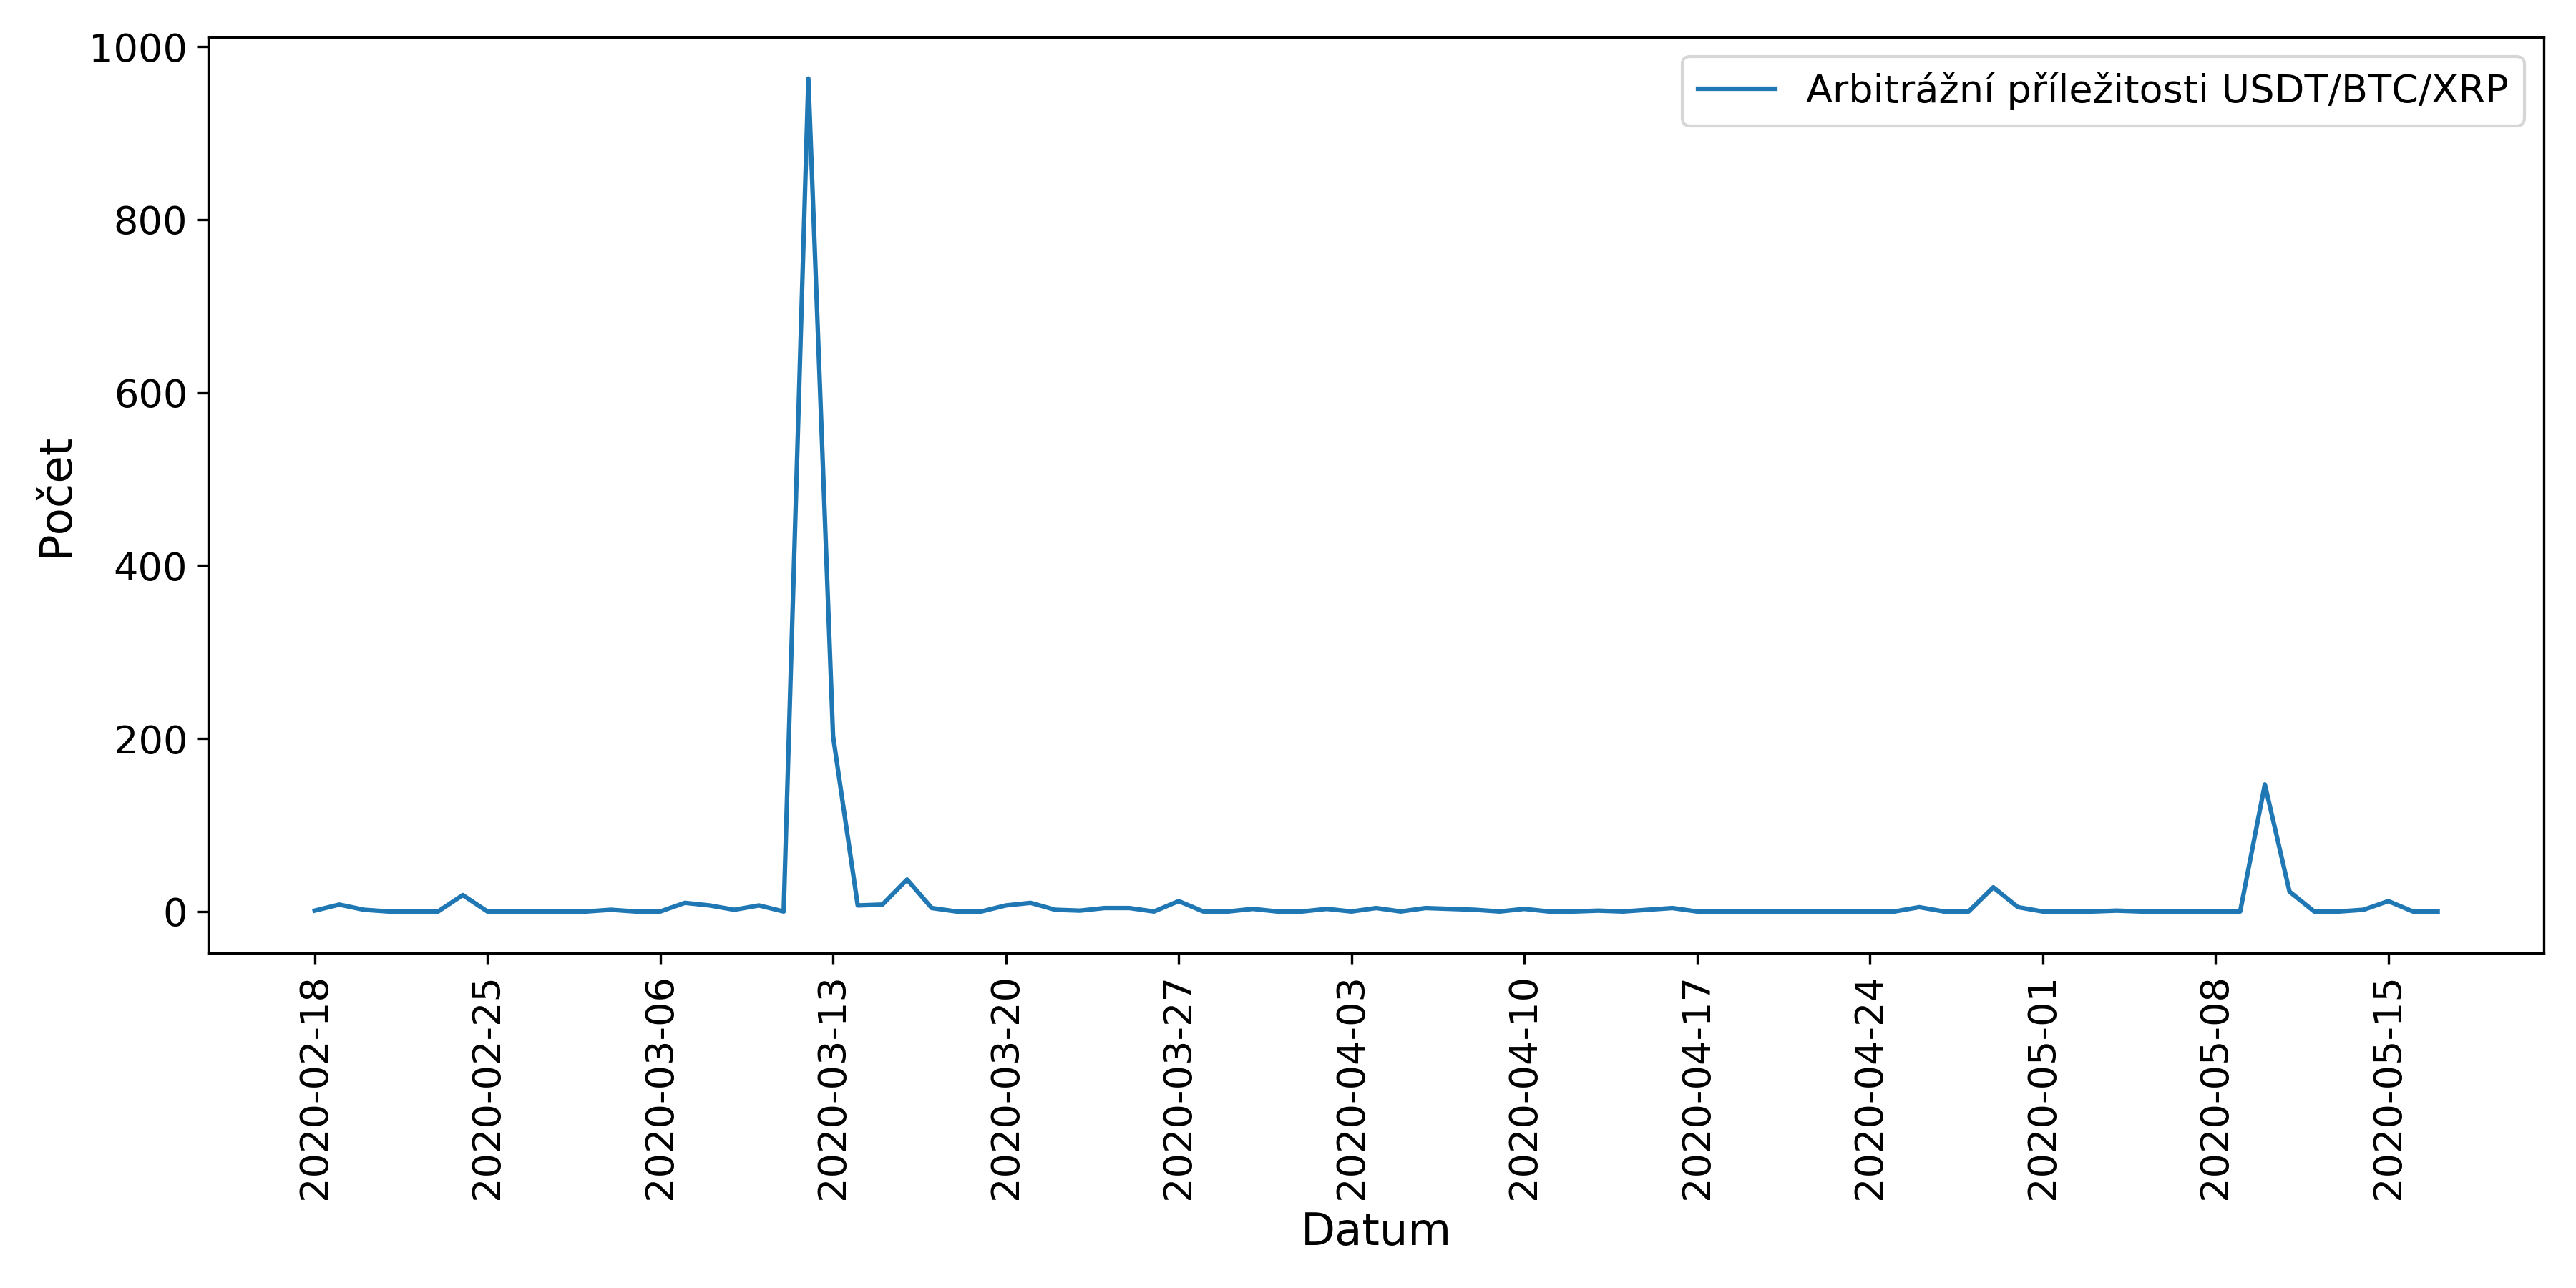
\includegraphics[width=1\textwidth]{images/best_triangles/occurences_arbitrage_USDTBTCXRP.png}
	\caption{Vývoj arbitrážních příležitostí na~trojúhelníku USDT/BTC/XRP }\label{occurences_arbitrage_USDTBTCXRP}
\end{figure}

\subsubsection{Trojúhelník USDT/BTC/TRX}
Trojúhelník USDT/BTC/TRX je pátým nejvýnosnějším trojúhelníkem a svými vlastnostmi je opět velmi podobný všem výše zmíněným (viz tabulka \ref{USDTBTCTRX_stats}). Denní průměr výdělku je poměrně vysoký (105~USD) na to, že se průměrně za den objeví pouze necelých sedm arbitrážních příležitostí. Medián výskytu arbitrážních příležitostí je 0, tedy během většiny dní se na tomto trojúhelníku nic zajímavého neděje. Nejvýnosnější arbitrážní příležitostí bylo možné vydělat 5,5~\% celkové potenciální zisku za pozorovanou dobu.. 

\begin{table}\centering
\caption{Základní statistiky trojúhelníku USDT/BTC/TRX}
\label{USDTBTCTRX_stats}
\begin{tabular}{|| l | r ||}
\hline Název & Hodnota \\ 
\hline\hline Název & USDT/BTC/TRX \\ 
\hline Počet dní & 87 \\ 
\hline Průměrný denní počet arbitráží & 6,32183908045977 \\ 
\hline Medián denního počtu arbitráží & 0,0 \\ 
\hline Průměrný procentuální zisk & 1,0005649956765 \\ 
\hline Nejvyšší procentuální zisk & 1,081229127 \\ 
\hline Celkový potenciální zisk & 725679,610703 TRX \\ 
\hline Celkový potenciální zisk (USD) & 9141,38605602326 \\ 
\hline Průměrný denní potenciální zisk & 8341,144951 TRX \\ 
\hline Průměrný denní potenciální zisk (USD) & 105,0734029427961 \\ 
\hline Nejvyšší potenciální zisk & 35482,621400 TRX \\ 
\hline Nejvyšší potenciální zisk (USD) & 446,97458177580006 \\ 
\hline Průměrná doba trvání & 0,37156302745091413 \\ 
\hline Celkový počet příležitostí & 931 \\ 
\hline Počet příležitostí k zisku poloviny celkového zisku & 27 \\ 
\hline
\end{tabular}
\end{table}

\begin{figure}\centering
	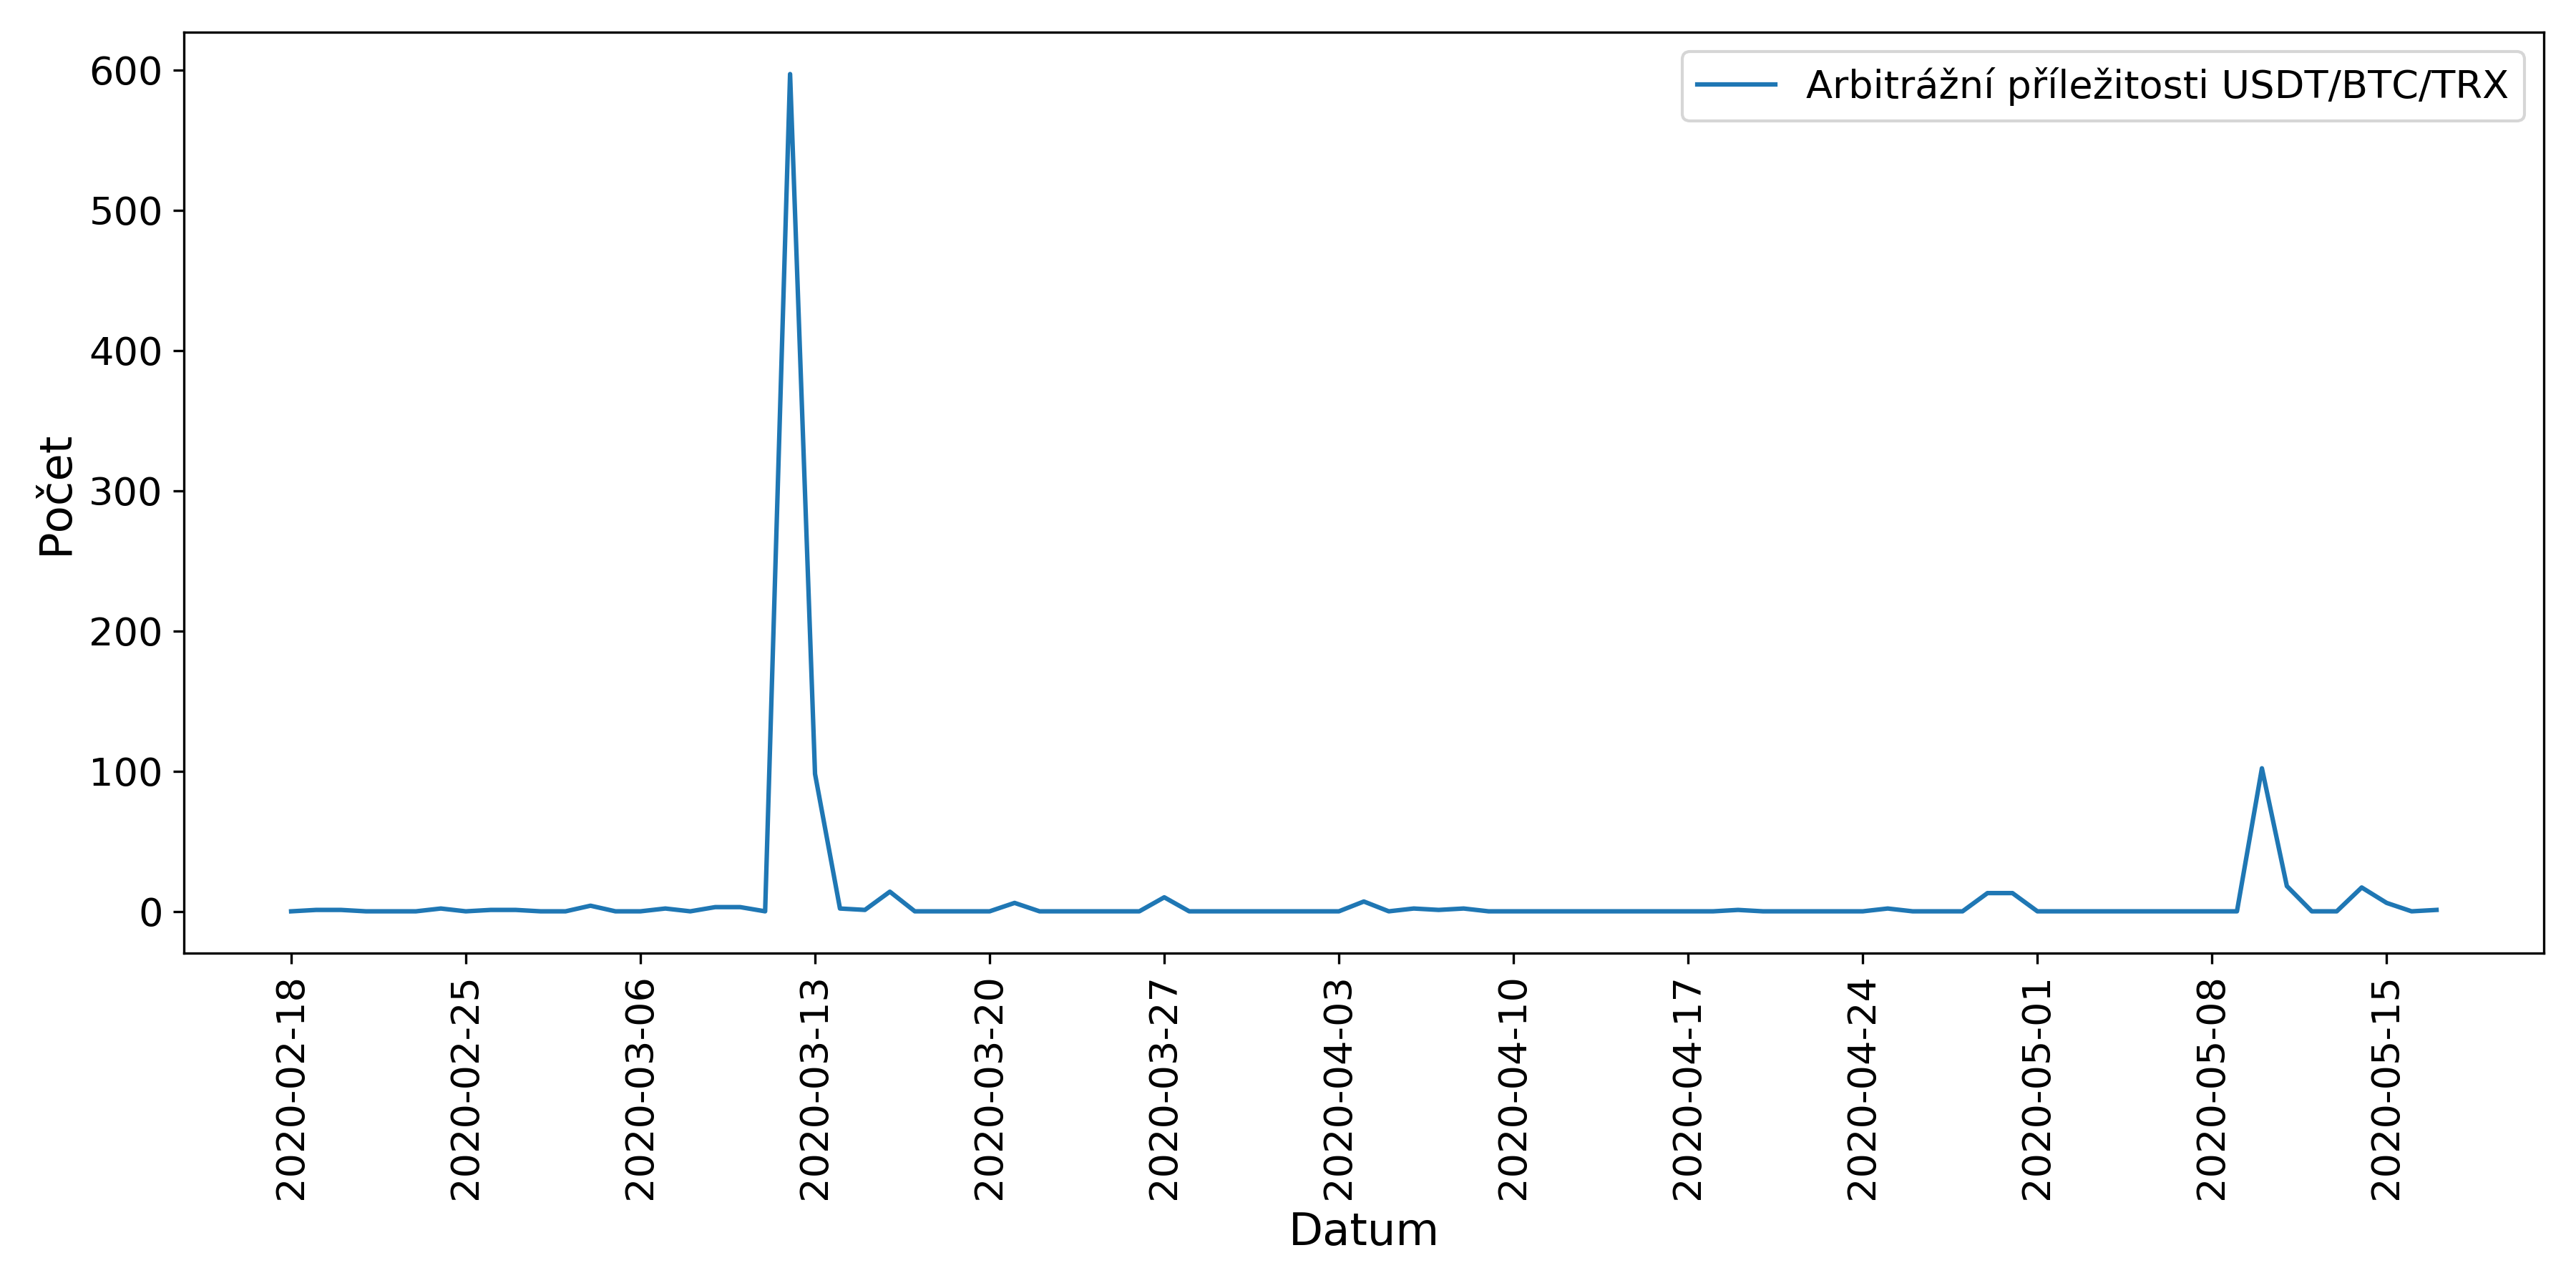
\includegraphics[width=1\textwidth]{images/best_triangles/occurences_arbitrage_USDTBTCTRX.png}
	\caption{Vývoj arbitrážních příležitostí na~trojúhelníku USDT/BTC/TRX }\label{occurences_arbitrage_USDTBTCTRX}
\end{figure}

\subsubsection{Trojúhelník USDT/BTC/BCH}
Trojúhelník USDT/BTC/XRP je sice posledním trojúhelníkem splňujícím podmínku průměrné denní výdělečnosti přes 10~amerických dolarů, je na druhou stranu zajímavý svými hodnotami. Celkově se na tomto trojúhelníku průměrně vyskytuje ani ne 5 pozitivních arbitrážních příležitostí denně. Zajímavý je tím, že na jeho nejvýdělečnější transakci bylo možné vydělat 0,61~BCH, což odpovídá 36,7~\% celkového potenciálního zisku za měřený úsek (viz tabulka \ref{USDTBTCBCH_stats}).

\begin{table}\centering
\caption{Základní statistiky trojúhelníku USDT/BTC/BCH}
\label{USDTBTCBCH_stats}
\begin{tabular}{|| l | r ||}
\hline Název & Hodnota \\ 
\hline\hline Název & USDT/BTC/BCH \\ 
\hline Počet dní & 60 \\ 
\hline Průměrný denní počet arbitráží & 4,633333333333334 \\ 
\hline Medián denního počtu arbitráží & 0,0 \\ 
\hline Průměrný procentuální zisk & 1,0007975736975039 \\ 
\hline Nejvyšší procentuální zisk & 1,03076856 \\ 
\hline Celkový potenciální zisk & 4,812820 BCH \\ 
\hline Celkový potenciální zisk (USD) & 1073,1625924129744 \\ 
\hline Průměrný denní potenciální zisk & 0,080214 BCH \\ 
\hline Průměrný denní potenciální zisk (USD) & 17,886043206882906 \\ 
\hline Nejvyšší potenciální zisk & 0,611238 BCH \\ 
\hline Nejvyšší potenciální zisk (USD) & 136,29376486436797 \\ 
\hline Průměrná doba trvání & 0,37848524100832015 \\ 
\hline Celkový počet příležitostí & 296 \\ 
\hline Počet příležitostí k zisku poloviny celkového zisku & 8 \\ 
\hline
\end{tabular}
\end{table}

\begin{figure}\centering
	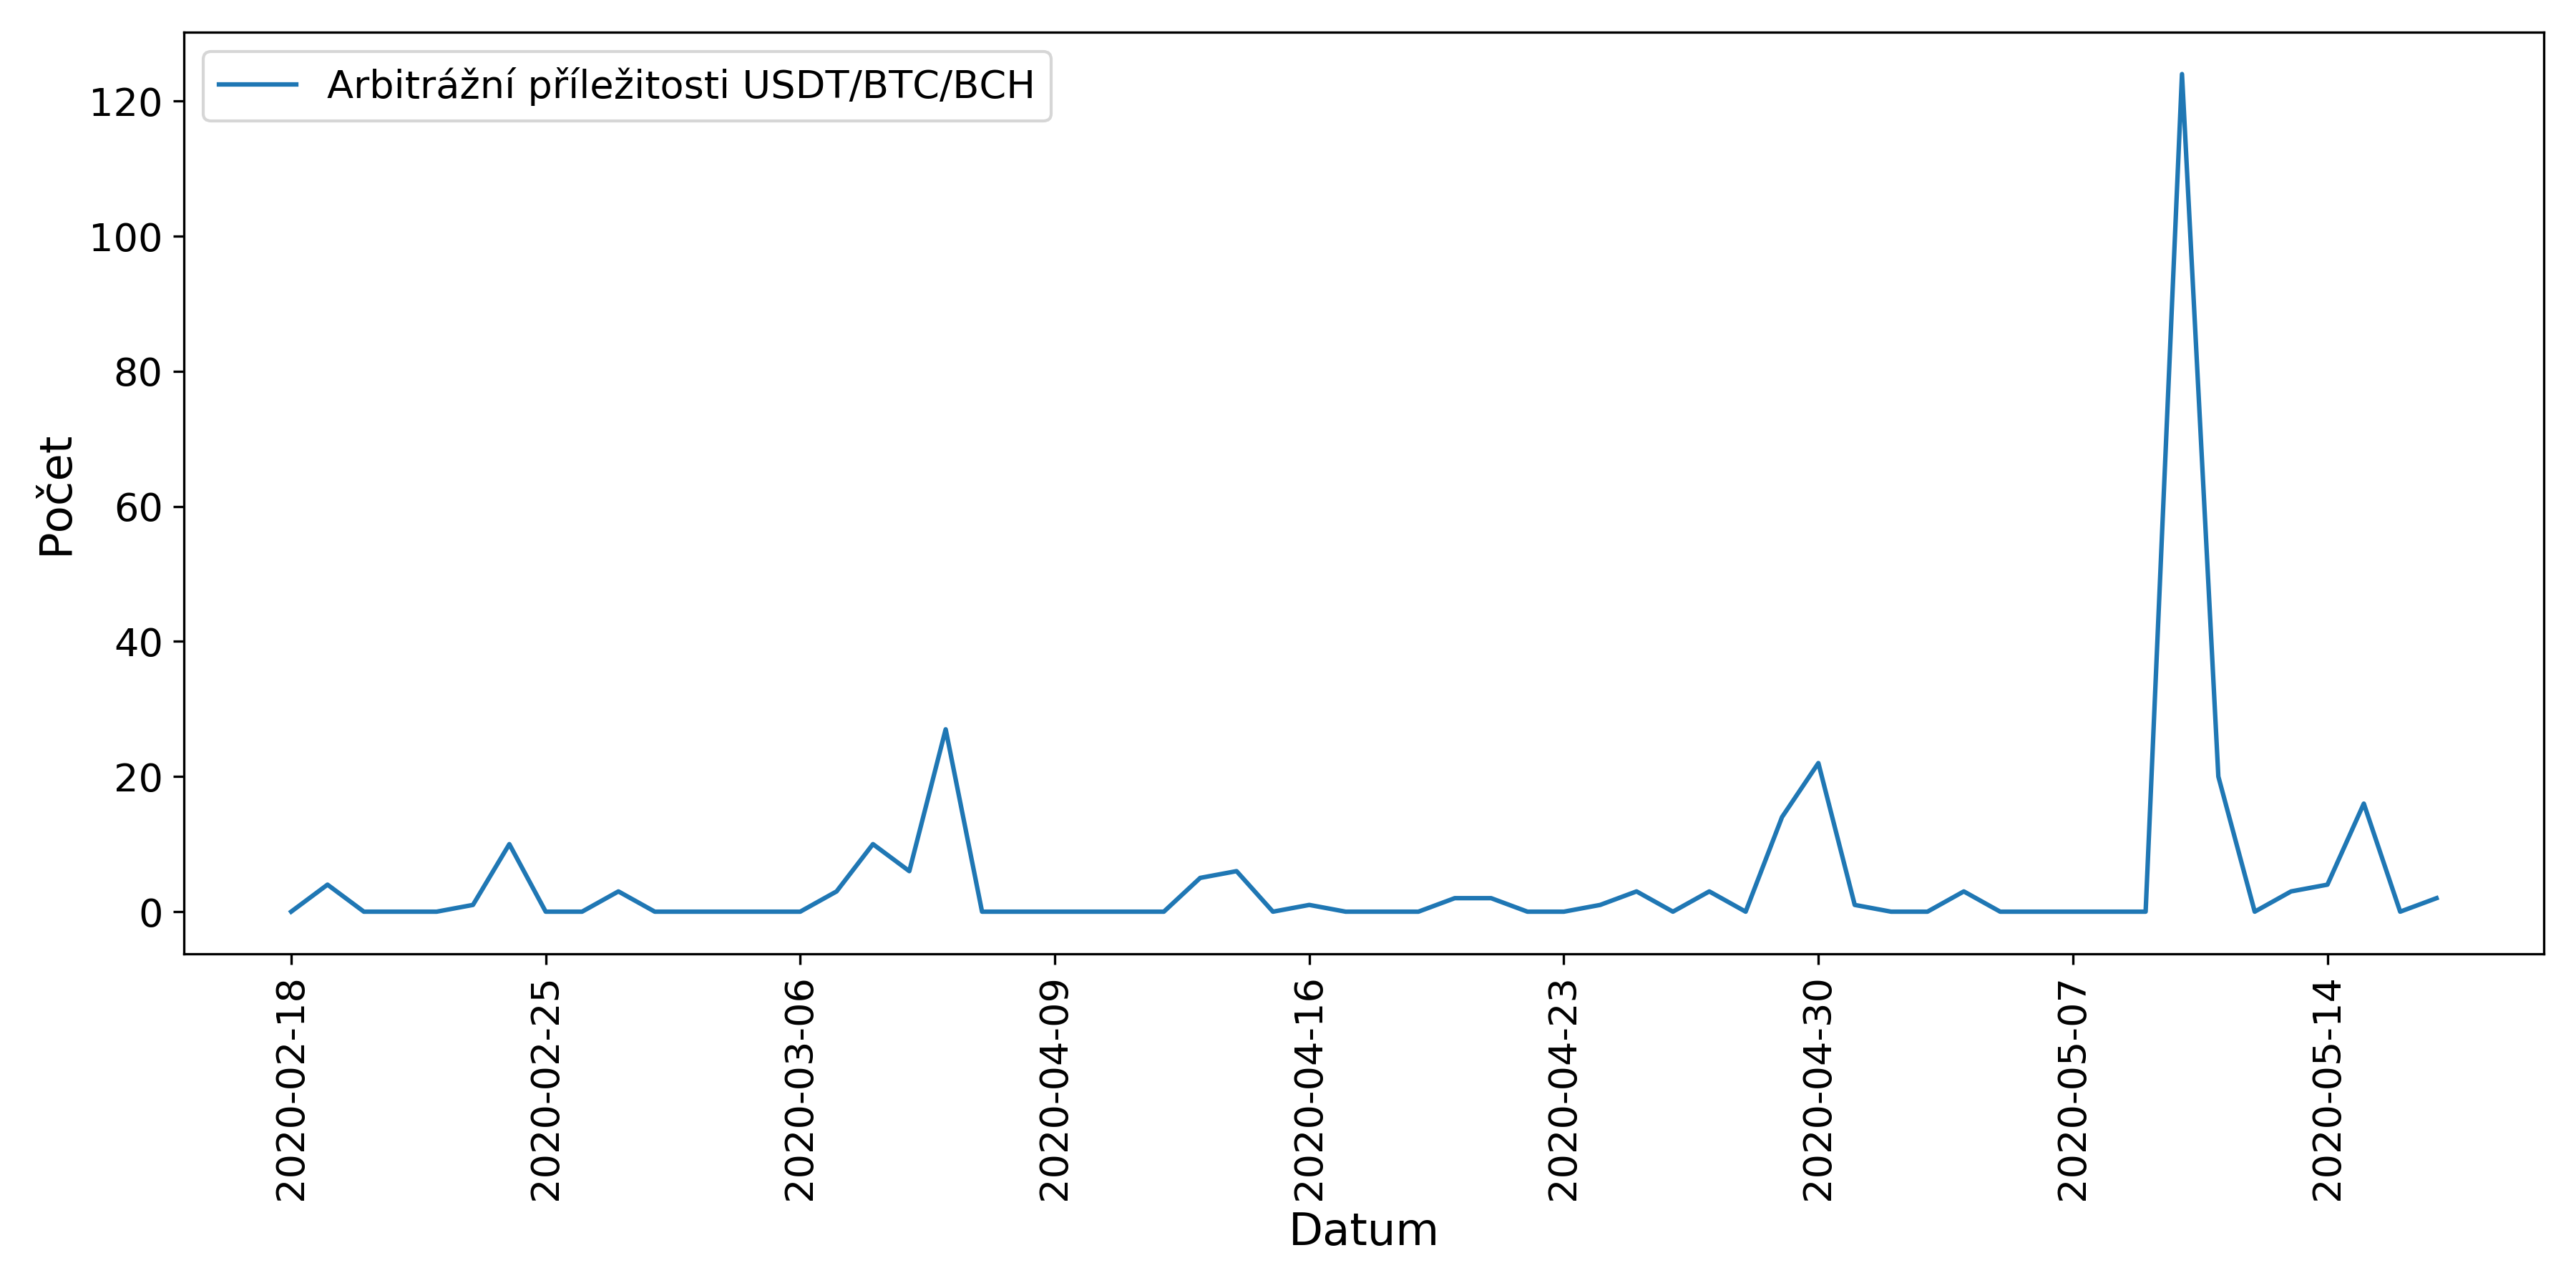
\includegraphics[width=1\textwidth]{images/best_triangles/occurences_arbitrage_USDTBTCBCH.png}
	\caption{Vývoj arbitrážních příležitostí na~trojúhelníku USDT/BTC/BCH }\label{occurences_arbitrage_USDTBTCBCH}
\end{figure}

\subsubsection{Zhodnocení nejlepších trojúhelníků}
Z předchozích podkapitol, kde se~blíže věnuji nejzajímavějším trojúhelníkům je vidět, že všechny mají velmi podobné vlastnosti, co se~týče data výskytu i~délky výskytu (viz spojený graf nejlepších trojúhelníků \ref{occurence_of_best}). Tento jev může být částečně způsobený tím, že ve~všech trojúhelnících figuruje USD Tether. 

Neboť průměrná doba životnosti arbitrážní příležitosti v~žádném případě ani nedosahuje jedné vteřiny, není reálně možné detekovat a~vytěžit arbitrážní příležitosti ručně bez jakéhokoliv bota, který by se~staral o~detekci a~následné vytěžování. 

Dále je nutné podotknout, že pro zobchodování některých arbitrážních příležitostí by bylo nutné zobchodovat jmění o objemech několika desítek tisíc amerických dolarů. Jelikož na téměř všech výdělečných trojúhelnících figuruje USDT stačí mít teoreticky pro vytěžování většiny trojúhelníků velký obnos pouze v této měně.

\begin{figure}\centering
	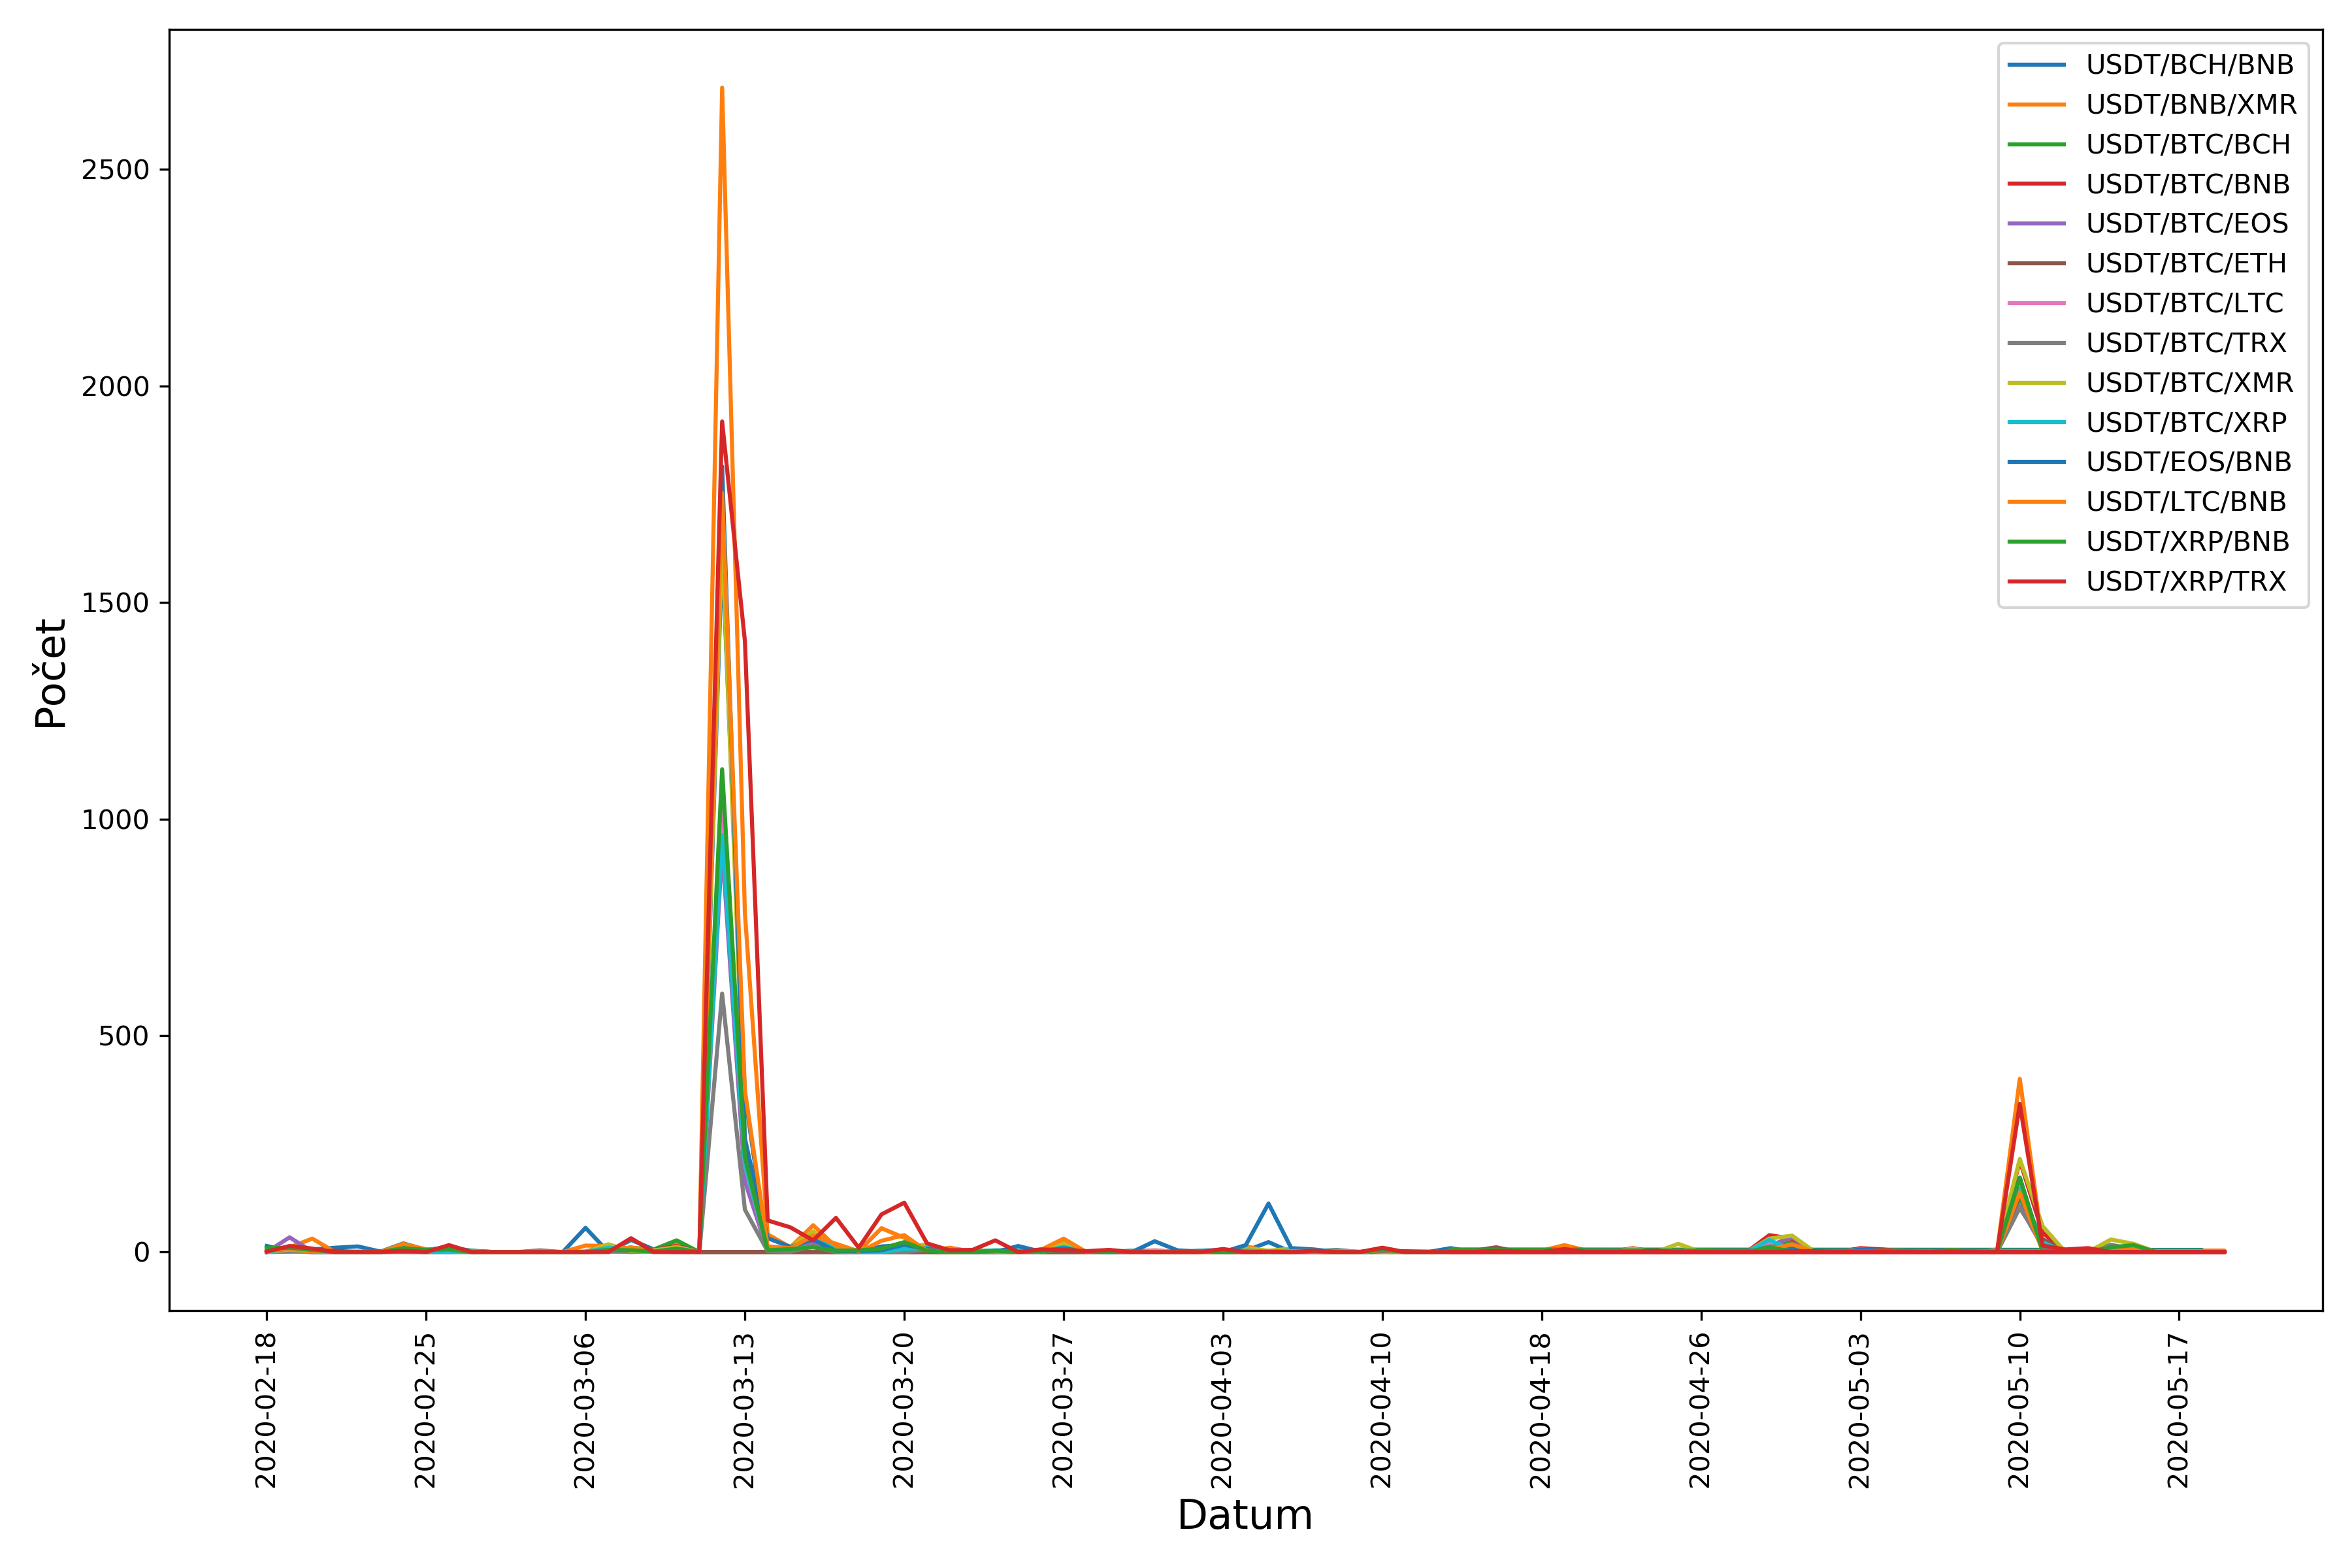
\includegraphics[width=1\textwidth]{images/best_triangles/occurence_of_best.png}
	\caption{Srovnání vývoje denního výskytu arbitrážních příležitostí na nejlepších trojúhelnících }\label{occurence_of_best}
\end{figure}

% todo - Změnit celý závěr
\begin{conclusion}
Cílem práce bylo zanalyzovat arbitrážní příležitosti kryptoměn a na základě reálných dat z kryptoměnových burz vyhodnotit základní statistiky výskytu a výdělečnosti.

Do teoretické části jsem popsal historii bitcoinu a rozebral jsem jeho princip a základní technologie. Dále jsem se zaměřil na několik altcoinů a několik kryptoměnových burz a zaobíral jsem se tématem arbitrážních příležitostí. 

V praktické části jsem úspěšně implementoval program, který sbíral data z~burzy Binance. Na datech jsem následně vyhledával trojúhelníkové arbitrážní příležitosti, které jsem v poslední části své bakalářské práce vyhodnocoval. 

Po nalezení arbitrážních příležitostí jsem se v rámci analytické části věnoval statistikám výskytů a výdělečnosti arbitrážních příležitostí, ke kterým jsem využíval tabulky a grafy vytvořené z nasbíraných dat. Zabýval jsem se selekcí těch nejlepších trojúhelníků z pohledu jejich výdělečnosti a potenciální vytěžitelnosti.

Ze statistik jsem zjistil, že problematika trojúhelníkových arbitrážních příležitostí je stále aktuální a je na ni možné vydělat poměrně velké množství peněz. Úkol vydělávání se však nyní stává náročnější z důvodu krátké životnosti arbitrážních příležitostí, kterou člověk nemá šanci sledovat dostatečně rychle bez využití počítačové síly.

Práci je možné dále rozšířit, převážně části závisející na sběru dat. V rámci bakalářské práce jsem neměl dostatek času na vytvoření větší datové kolekce a~tří měsíční data nebyla dostatečně rozmanitá k vyhodnocení některých závěrů převážně v částech hodnotících korelace s arbitrážními příležitostmi.

V rámci své práce jsem se nevěnoval reálnému vytěžování pozitivních arbitrážních příležitostí, které si však plánuji na základě zjištěných závěrů v~budoucnu vytvořit. Data ze skutečného vytěžování arbitrážních příležitostí by bylo také zajímavé zahrnout do analytické části práce.

\end{conclusion}

% \bibliographystyle{csn690}
% \bibliography{mybibliographyfile}

\printbibliography

\appendix

\chapter{Seznam použitých zkratek}
% \printglossaries
\begin{description}
	\item[BTC] Bitcoin
	\item[LTC] Linecoin
	\item[ETH] Ethereum
	\item[TRX] TRON
	\item[XMR] Monero
	\item[USDT] USD Tether
	\item[BNB] Binance coin
	\item[BCH] Bitcoin Cash
	\item[XRP] Ripple
	\item[API] Application Program Interface
\end{description}


% % % % % % % % % % % % % % % % % % % % % % % % % % % % 
% % Tuto kapitolu z~výsledné práce ODSTRAŇTE.
% % % % % % % % % % % % % % % % % % % % % % % % % % % % 
% 
% \chapter{Návod k~použití této šablony}
% 
% Tento dokument slouží jako základ pro napsání závěrečné práce na~Fakultě informačních technologií ČVUT v~Praze.
% 
% \section{Výběr základu}
% 
% Vyberte si šablonu podle druhu práce (bakalářská, diplomová), jazyka (čeština, angličtina) a~kódování (ASCII, \mbox{UTF-8}, \mbox{ISO-8859-2} neboli latin2 a~nebo \mbox{Windows-1250}). 
% 
% V~české variantě naleznete šablony v~souborech pojmenovaných ve~formátu práce\_kódování.tex. Typ může být:
% \begin{description}
% 	\item[BP] bakalářská práce,
% 	\item[DP] diplomová (magisterská) práce.
% \end{description}
% Kódování, ve~kterém chcete psát, může být:
% \begin{description}
% 	\item[UTF-8] kódování Unicode,
% 	\item[ISO-8859-2] latin2,
% 	\item[Windows-1250] znaková sada 1250 Windows.
% \end{description}
% V~případě nejistoty ohledně kódování doporučujeme následující postup:
% \begin{enumerate}
% 	\item Otevřete šablony pro kódování UTF-8 v~editoru prostého textu, který chcete pro psaní práce použít -- pokud můžete texty s~diakritikou normálně přečíst, použijte tuto šablonu.
% 	\item V~opačném případě postupujte dále podle toho, jaký operační systém používáte:
% 	\begin{itemize}
% 		\item v~případě Windows použijte šablonu pro kódování \mbox{Windows-1250},
% 		\item jinak zkuste použít šablonu pro kódování \mbox{ISO-8859-2}.
% 	\end{itemize}
% \end{enumerate}
% 
% 
% V~anglické variantě jsou šablony pojmenované podle typu práce, možnosti jsou:
% \begin{description}
% 	\item[bachelors] bakalářská práce,
% 	\item[masters] diplomová (magisterská) práce.
% \end{description}
% 
% \section{Použití šablony}
% 
% Šablona je určena pro zpracování systémem \LaTeXe{}. Text je možné psát v~textovém editoru jako prostý text, lze však také využít specializovaný editor pro \LaTeX{}, např. Kile.
% 
% Pro získání tisknutelného výstupu z~takto vytvořeného souboru použijte příkaz \verb|pdflatex|, kterému předáte cestu k~souboru jako parametr. Vhodný editor pro \LaTeX{} toto udělá za~Vás. \verb|pdfcslatex| ani \verb|cslatex| \emph{nebudou} s~těmito šablonami fungovat.
% 
% Více informací o~použití systému \LaTeX{} najdete např. V~\cite{wikilatex}.
% 
% \subsection{Typografie}
% 
% Při psaní dodržujte typografické konvence zvoleného jazyka. České \uv{uvozovky} zapisujte použitím příkazu \verb|\uv|, kterému v~parametru předáte text, jenž má být v~uvozovkách. Anglické otevírací uvozovky se~v~\LaTeX{}u zadávají jako dva zpětné apostrofy, uzavírací uvozovky jako dva apostrofy. Často chybně uváděný symbol "{} (palce) nemá s~uvozovkami nic společného.
% 
% Dále je třeba zabránit zalomení řádky mezi některými slovy, v~češtině např. Za~jednopísmennými předložkami a~spojkami (vyjma \uv{a}). To docílíte vložením pružné nezalomitelné mezery -- znakem \texttt{\textasciitilde}. V~tomto případě to není třeba dělat ručně, lze použít program \verb|vlna|.
% 
% Více o~typografii viz \cite{kobltypo}.
% 
% \subsection{Obrázky}
% 
% Pro umožnění vkládání obrázků je vhodné použít balíček \verb|graphicx|, samotné vložení se~provede příkazem \verb|\includegraphics|. Takto je možné vkládat obrázky ve~formátu PDF, PNG a~JPEG jestliže používáte pdf\LaTeX{} nebo ve~formátu EPS jestliže používáte \LaTeX{}. Doporučujeme preferovat vektorové obrázky před rastrovými (vyjma fotografií).
% 
% \subsubsection{Získání vhodného formátu}
% 
% Pro získání vektorových formátů PDF nebo EPS z~jiných lze použít některý z~vektorových grafických editorů. Pro převod rastrového obrázku na~vektorový lze použít rasterizaci, kterou mnohé editory zvládají (např. Inkscape). Pro konverze lze použít též nástroje pro dávkové zpracování běžně dodávané s~\LaTeX{}em, např. \verb|epstopdf|.
% 
% \subsubsection{Plovoucí prostředí}
% 
% Příkazem \verb|\includegraphics| lze obrázky vkládat přímo, doporučujeme však použít plovoucí prostředí, konkrétně \verb|figure|. Například obrázek \ref{fig:float} byl vložen tímto způsobem. Vůbec přitom nevadí, když je obrázek umístěn jinde, než bylo původně zamýšleno -- je tomu tak hlavně kvůli dodržení typografických konvencí. Namísto vynucování konkrétní pozice obrázku doporučujeme používat odkazování z~textu (dvojice příkazů \verb|\label| a~\verb|\ref|).
% 
% \begin{figure}\centering
% 	
\includegraphics[width=0.5\textwidth, angle=30]{cvut-logo-bw}
% 	\caption[Příklad obrázku]{Ukázkový obrázek v~plovoucím prostředí}\label{fig:float}
% \end{figure}
% 
% \subsubsection{Verze obrázků}
% 
% % Gnuplot BW i~barevně
% Může se~hodit mít více verzí stejného obrázku, např. pro barevný či černobílý tisk a~nebo pro prezentaci. S~pomocí některých nástrojů na~generování grafiky je to snadné.
% 
% Máte-li například graf vytvořený v~programu Gnuplot, můžete jeho černobílou variantu (viz obr. \ref{fig:gnuplot-bw}) vytvořit parametrem \verb|monochrome dashed| příkazu \verb|set term|. Barevnou variantu (viz obr. \ref{fig:gnuplot-col}) vhodnou na~prezentace lze vytvořit parametrem \verb|colour solid|.
% 
% \begin{figure}\centering
% 	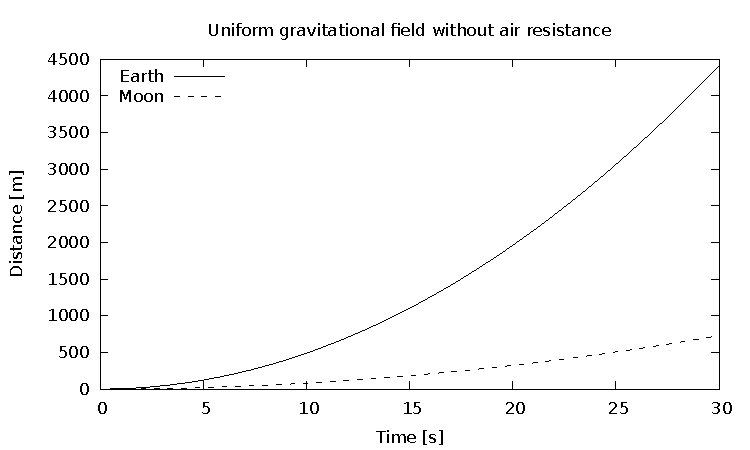
\includegraphics{gnuplot-bw}
% 	\caption{Černobílá varianta obrázku generovaného programem Gnuplot}\label{fig:gnuplot-bw}
% \end{figure}
% 
% \begin{figure}\centering
% 	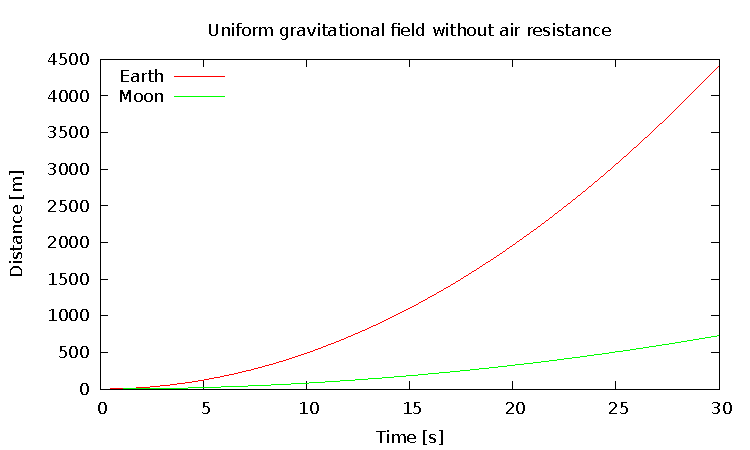
\includegraphics{gnuplot-col}
% 	\caption{Barevná varianta obrázku generovaného programem Gnuplot}\label{fig:gnuplot-col}
% \end{figure}
% 
% 
% \subsection{Tabulky}
% 
% Tabulky lze zadávat různě, např. V~prostředí \verb|tabular|, avšak pro jejich vkládání platí to samé, co pro obrázky -- použijte plovoucí prostředí, v~tomto případě \verb|table|. Například tabulka \ref{tab:matematika} byla vložena tímto způsobem.
% 
% % % % % % % % % % % % % % % % % % % % % % % % % % % % 

\chapter{Obsah přiloženého CD}

%upravte podle skutecnosti

\begin{figure}
	\dirtree{%
		.1 readme.txt\DTcomment{stručný popis obsahu CD}.
		.1 exe\DTcomment{adresář se~spustitelnou formou implementace}.
		.1 src.
		.2 impl\DTcomment{zdrojové kódy implementace}.
		.2 thesis\DTcomment{zdrojová forma práce ve~formátu \LaTeX{}}.
		.1 text\DTcomment{text práce}.
		.2 thesis.pdf\DTcomment{text práce ve~formátu PDF}.
		.2 thesis.ps\DTcomment{text práce ve~formátu PS}.
	}
\end{figure}

\end{document}